\chapter{Experimentaciones y Resultados}

En las siguientes imágenes el circulo blanco en las columnas de optimización discreta y de fabricación
representa un círculo de radio $80nm$, el radio de curvatura aplicado en el filtro 
$\widetilde{\boldsymbol{P}}$.

Para poder comparar nuestros resultados, en la bibliografía tenemos lo siguiente:

\begin{enumerate}

  \item En \cite{Christiansen2021} se optimiza un WDM con una región de diseño de 
        $2 \mu m \times 2 \mu m$ donde la guía de onda de entrada es de $299 nm$,
        la guía de onda de salida superior es de $299 nm$ y la guía de salida inferior de $356 nm$.
        Con esta configuración, el mejor diseño tiene una transmitancia de $0.86$ en el brazo inferior
        a $1300 nm$ y de $0.85$ en el brazo superior a $1550 nm$.

  \item Usando una simulación en SPINS, para el caso del \emph{bend} tenemos que el diseño intuitivo
        posee una transmitancia de $0.8389$ a $1550 nm$.
        En el mejor de mi conocimiento, no hay publicaciones recientes que muestren resultados
        explícitos en la optimización de un bend en un área de diseño de $2 \mu m \times 2 \mu m$.

\end{enumerate}

%Estructura:

%Párrafo de introducción

%1. Describir los equipos utilizados
%  - Nodo Tesla
%  - Nodo Ampere
%  - Nodo Quadro

%2. Resultados del Bend  
%  - Plot de la opt. continua  
%  - Plot de la opt. discreta  
%  - Plot de la opt. de fabricación  
%  - Plot resumen de L-BFGS-B  
%  - Plot resumen de G-CMA-ES  
%  - Plot resumen de G-PSO  
%  - Plot resumen de G-GA  
%  - Plot resumen de MMA  
%3. Resultados del WDM  
%  - Plot de la opt. continua  
%  - Plot de la opt. discreta  
%  - Plot de la opt. de fabricación  
%  - Plot resumen de L-BFGS-B  
%  - Plot resumen de G-CMA-ES  
%  - Plot resumen de G-PSO  
%  - Plot resumen de G-GA  
%  - Plot resumen de MMA  
%4. Mejores resultados (mejores diseños optenidos por cada algoritmo, mostrar su diseño normal,
%   expandido y contraído)  
%  - Plot de L-BFGS-B  
%  - Plot de G-CMA-ES  
%  - Plot de G-PSO  
%  - Plot de G-GA  
%  - Plot de MMA  
%5. Preparación para fabricación  

% Bend - L-BFGS-B
\begin{table}[ht]
    \centering
    \vspace*{-2.5cm}
    \hspace*{-3cm}
    \begin{tabular}{|c|c|c|c|}
    \hline 
    \emph{Seed} & Opt. continua & Opt. discreta &  Opt. de fabricación \\
    \hline
      \multirow{2}{*}{128} &
      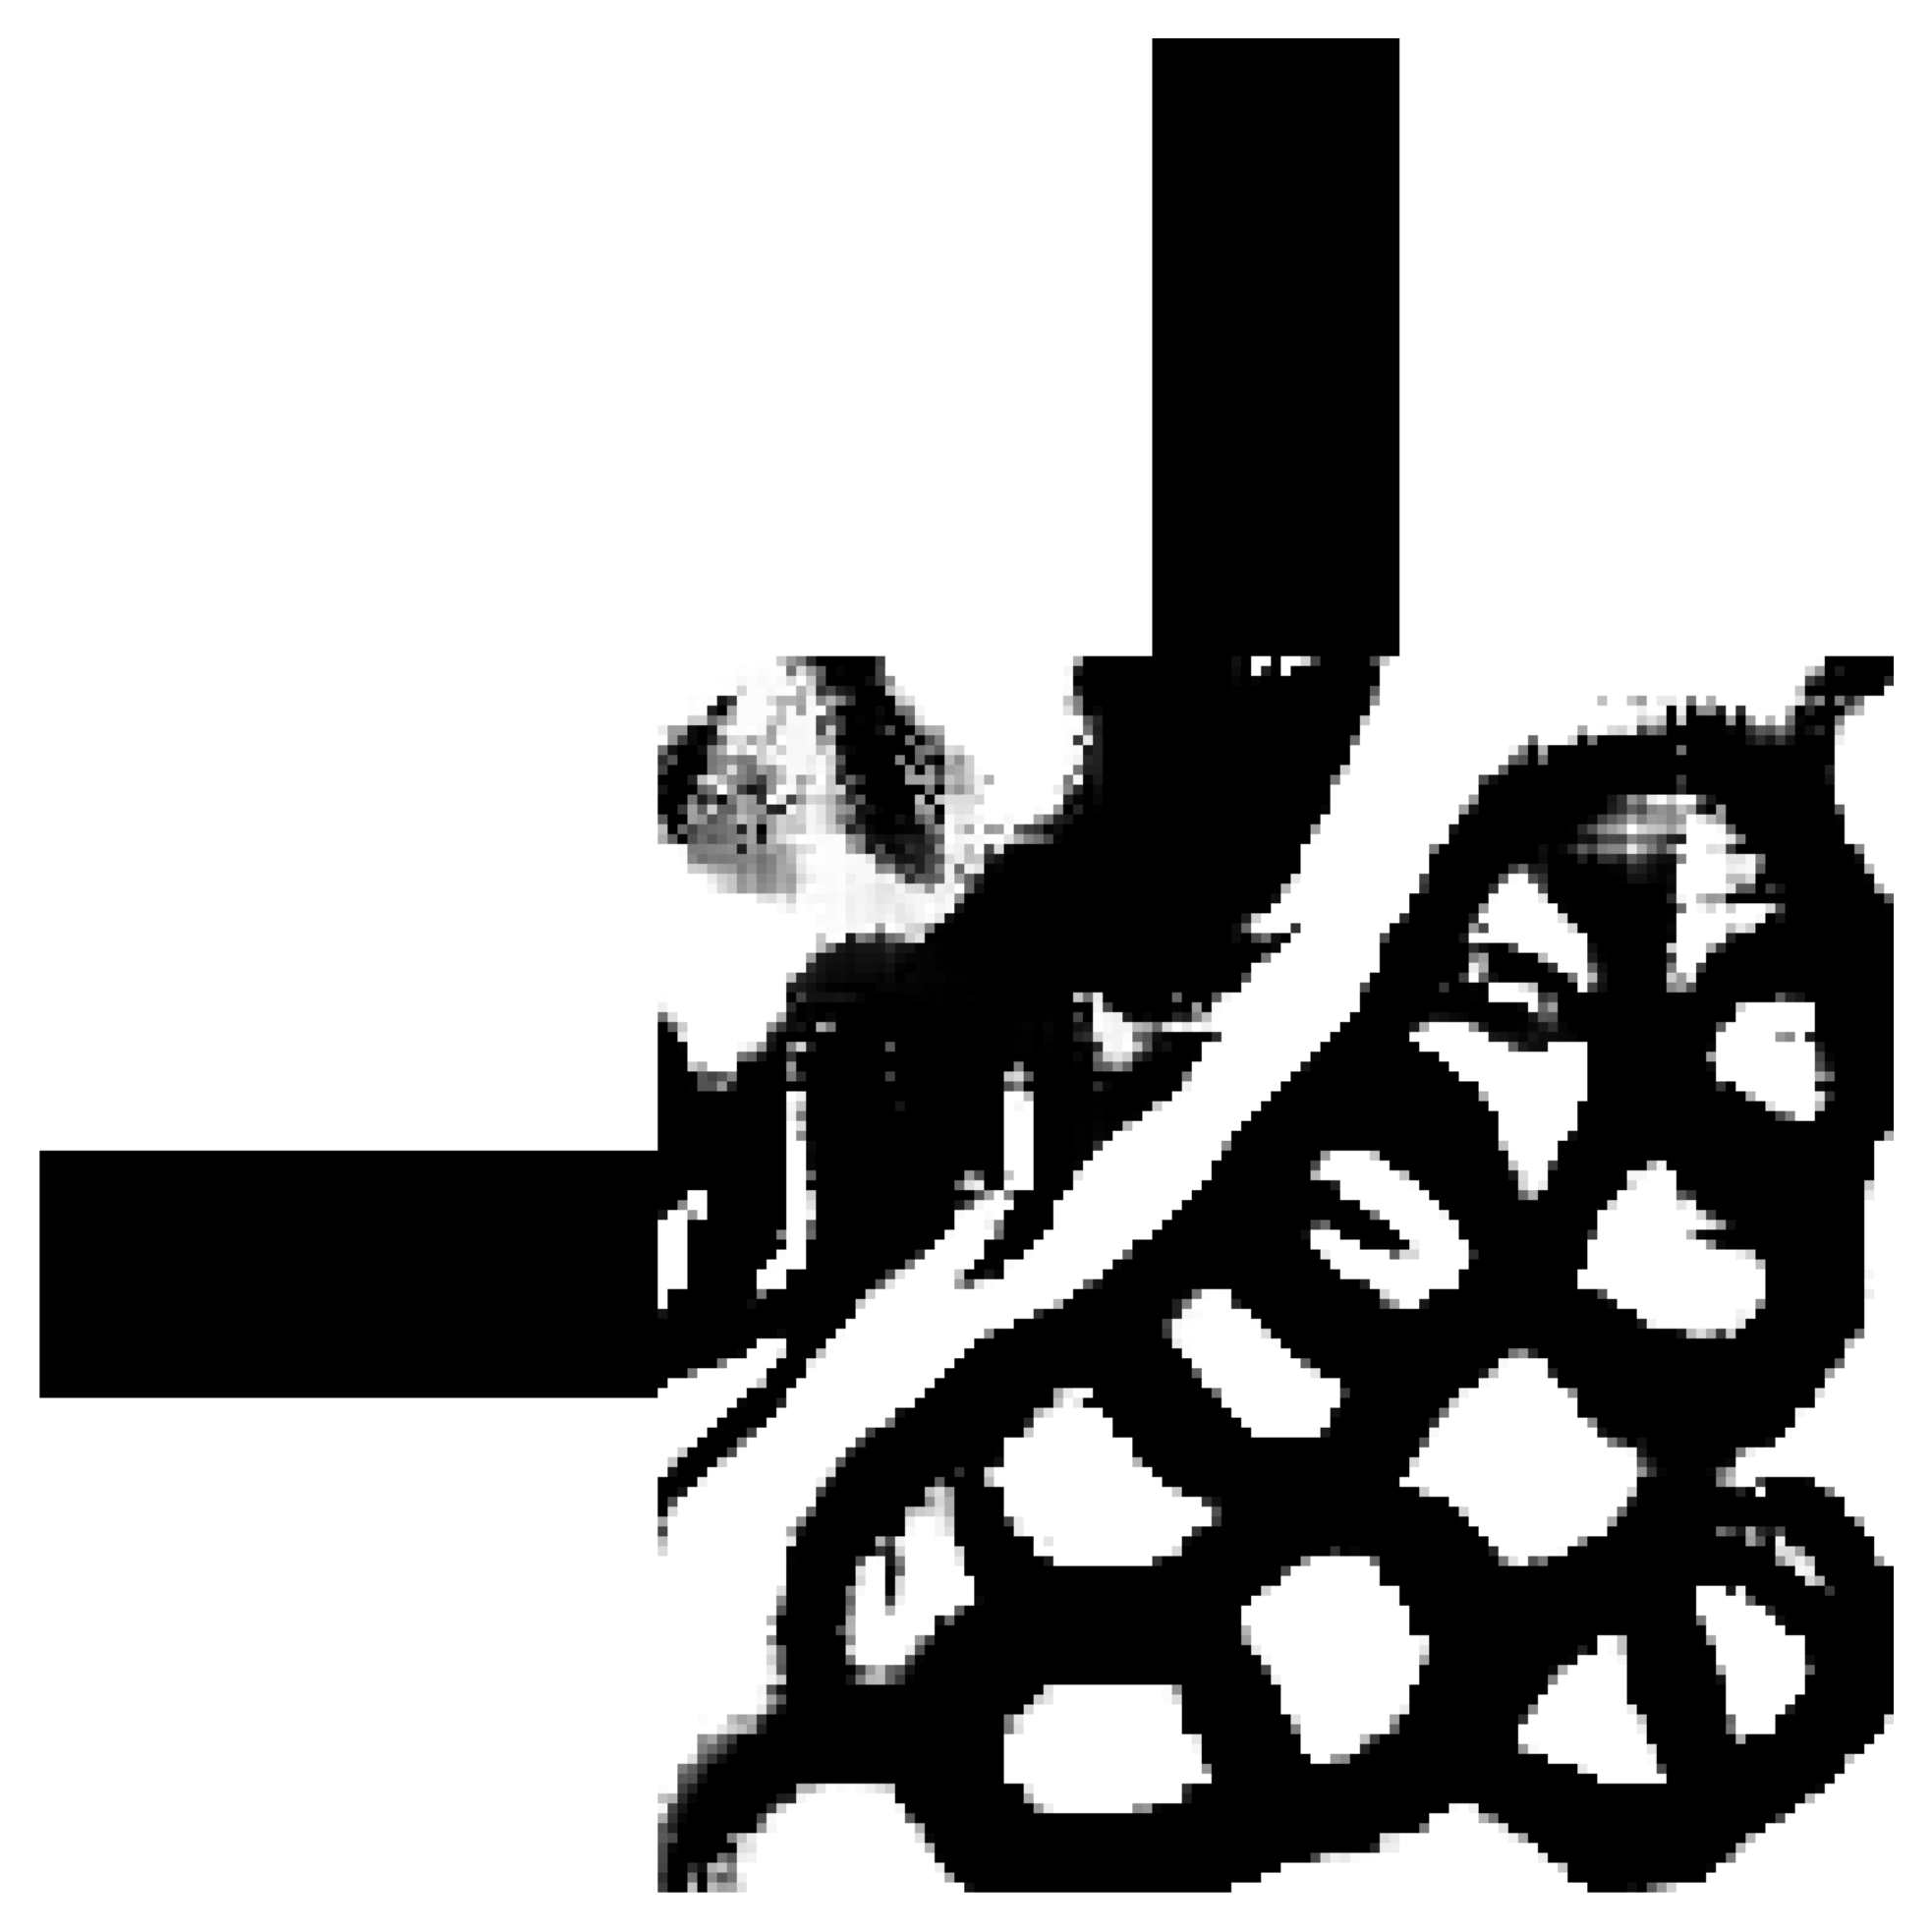
\includegraphics[width=0.20\textwidth]{image/results/bend/L-BFGS-B/visualize_eps_cont_128.png} &
      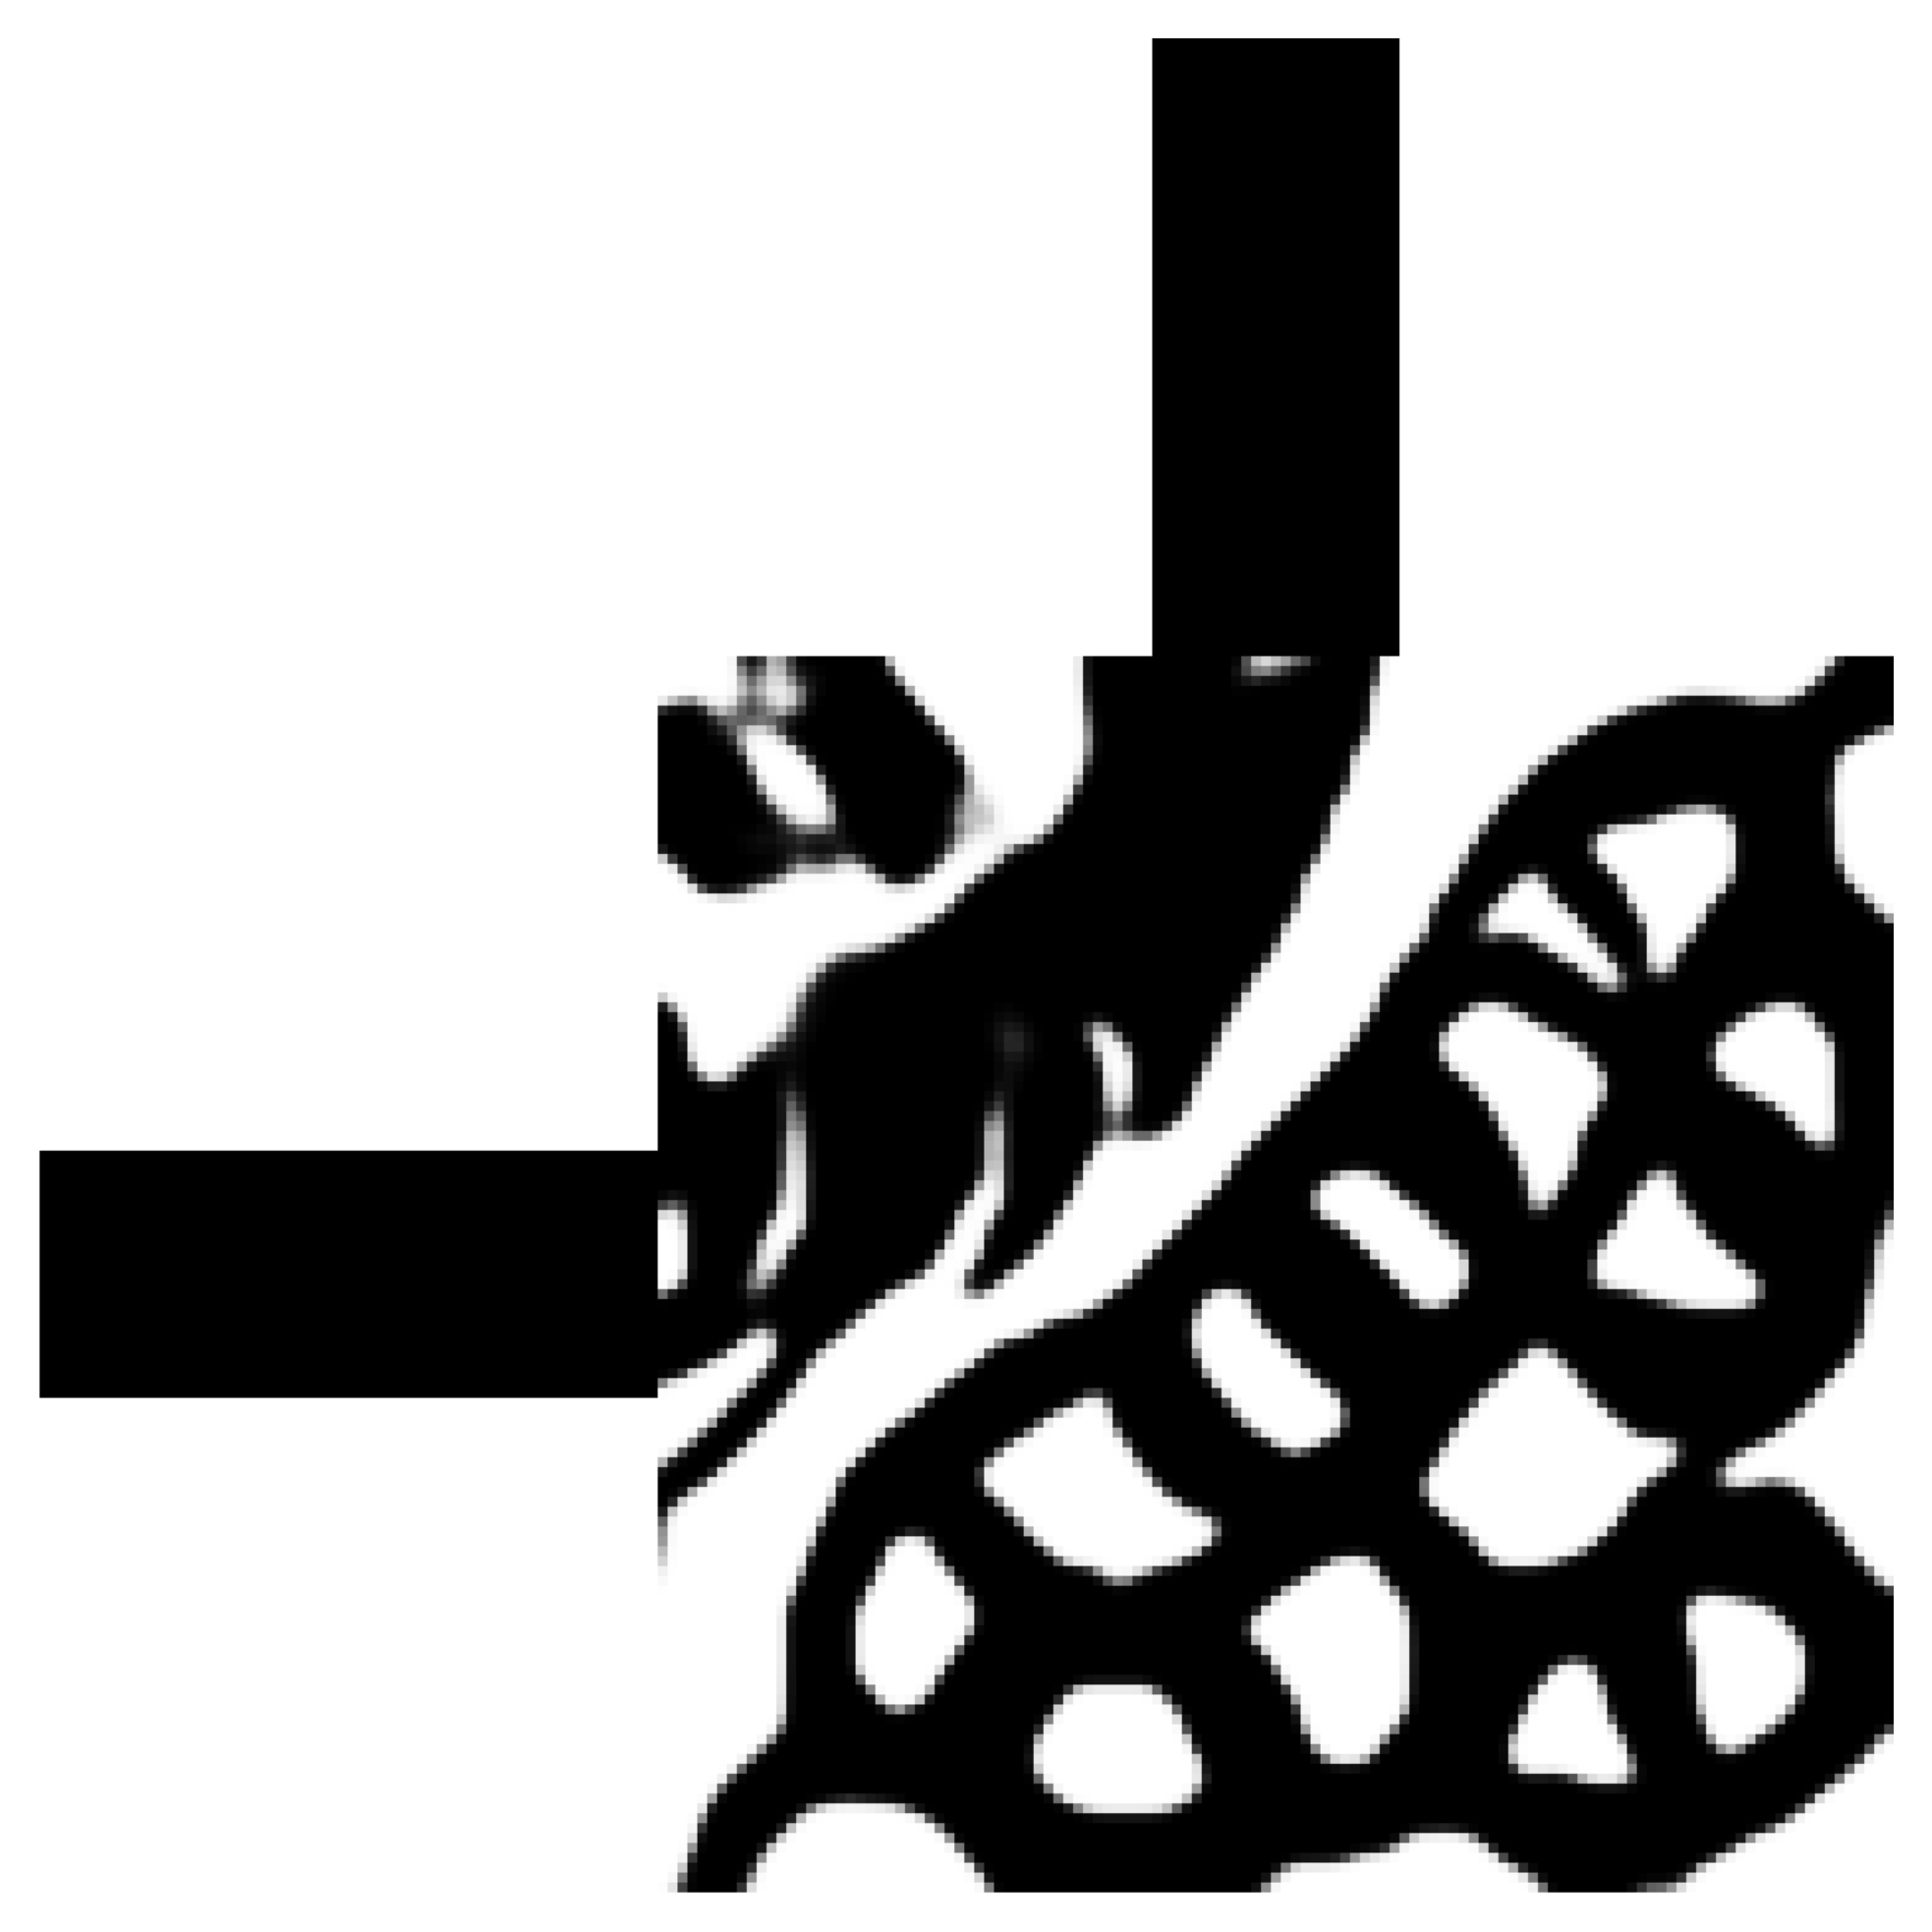
\includegraphics[width=0.20\textwidth]{image/results/bend/L-BFGS-B/visualize_eps_disc_128.png} &
      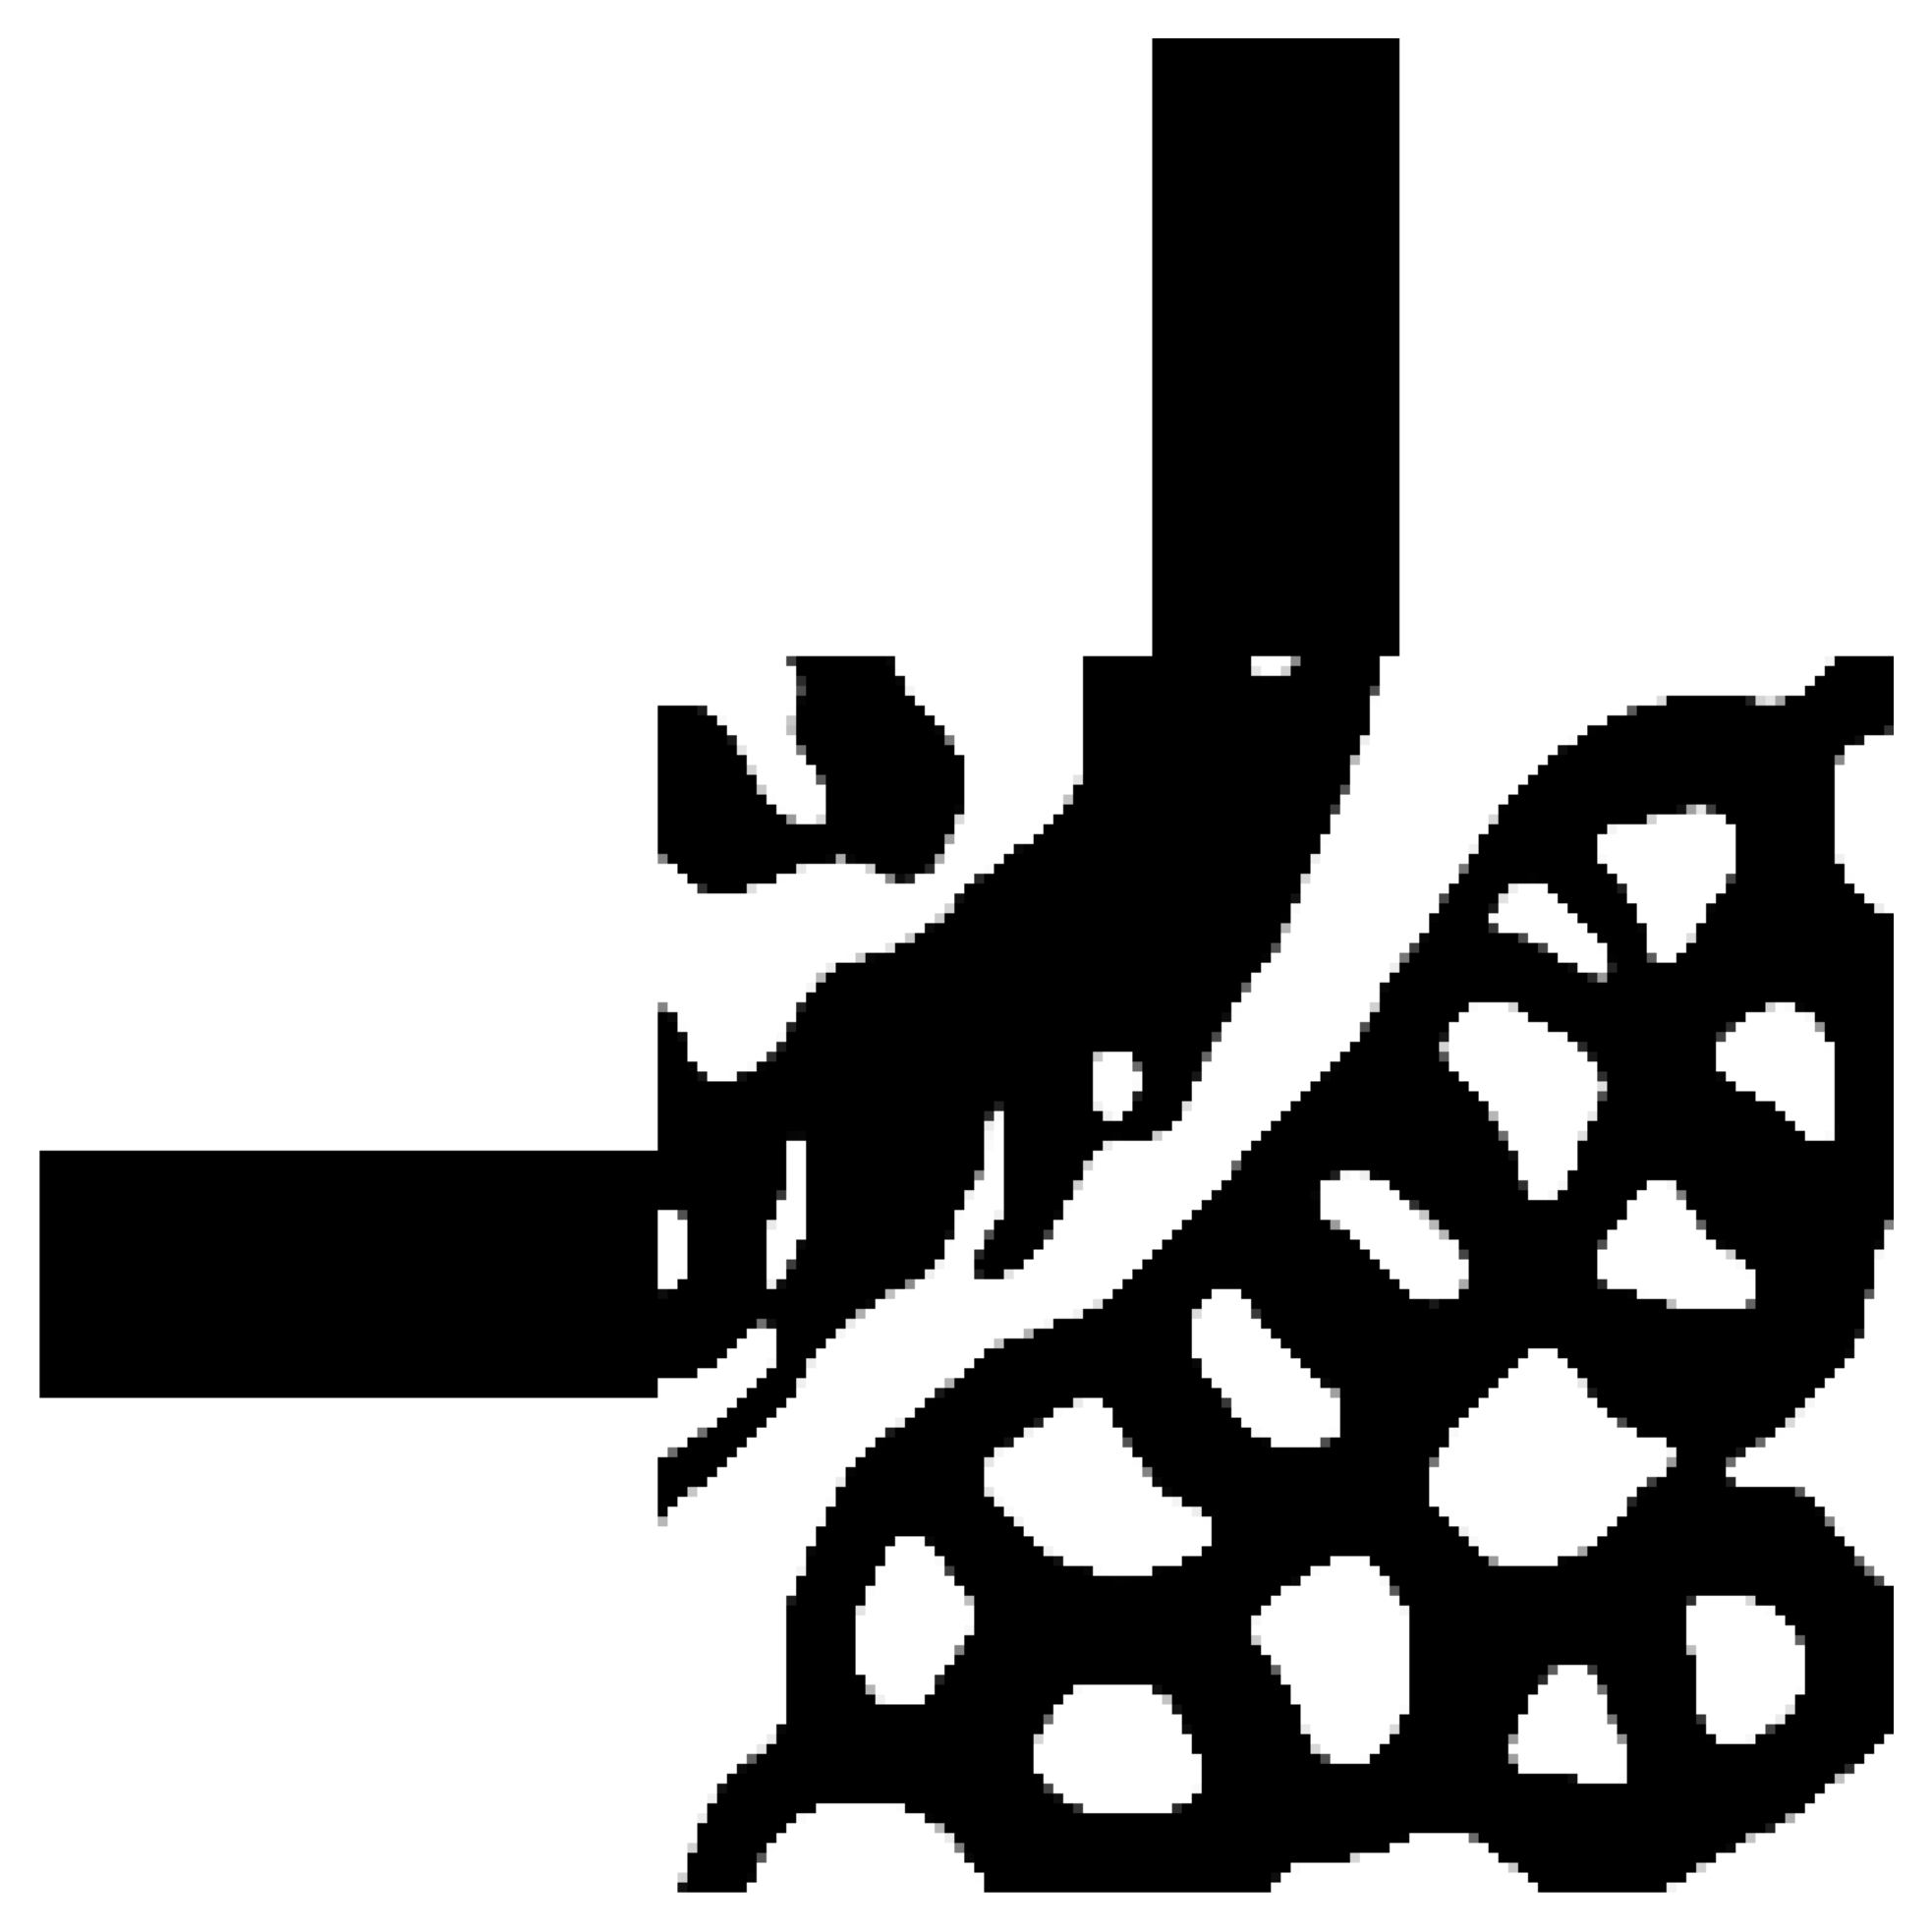
\includegraphics[width=0.20\textwidth]{image/results/bend/L-BFGS-B/visualize_eps_fab_128.png} \\
      \cline{2-4}
      &
      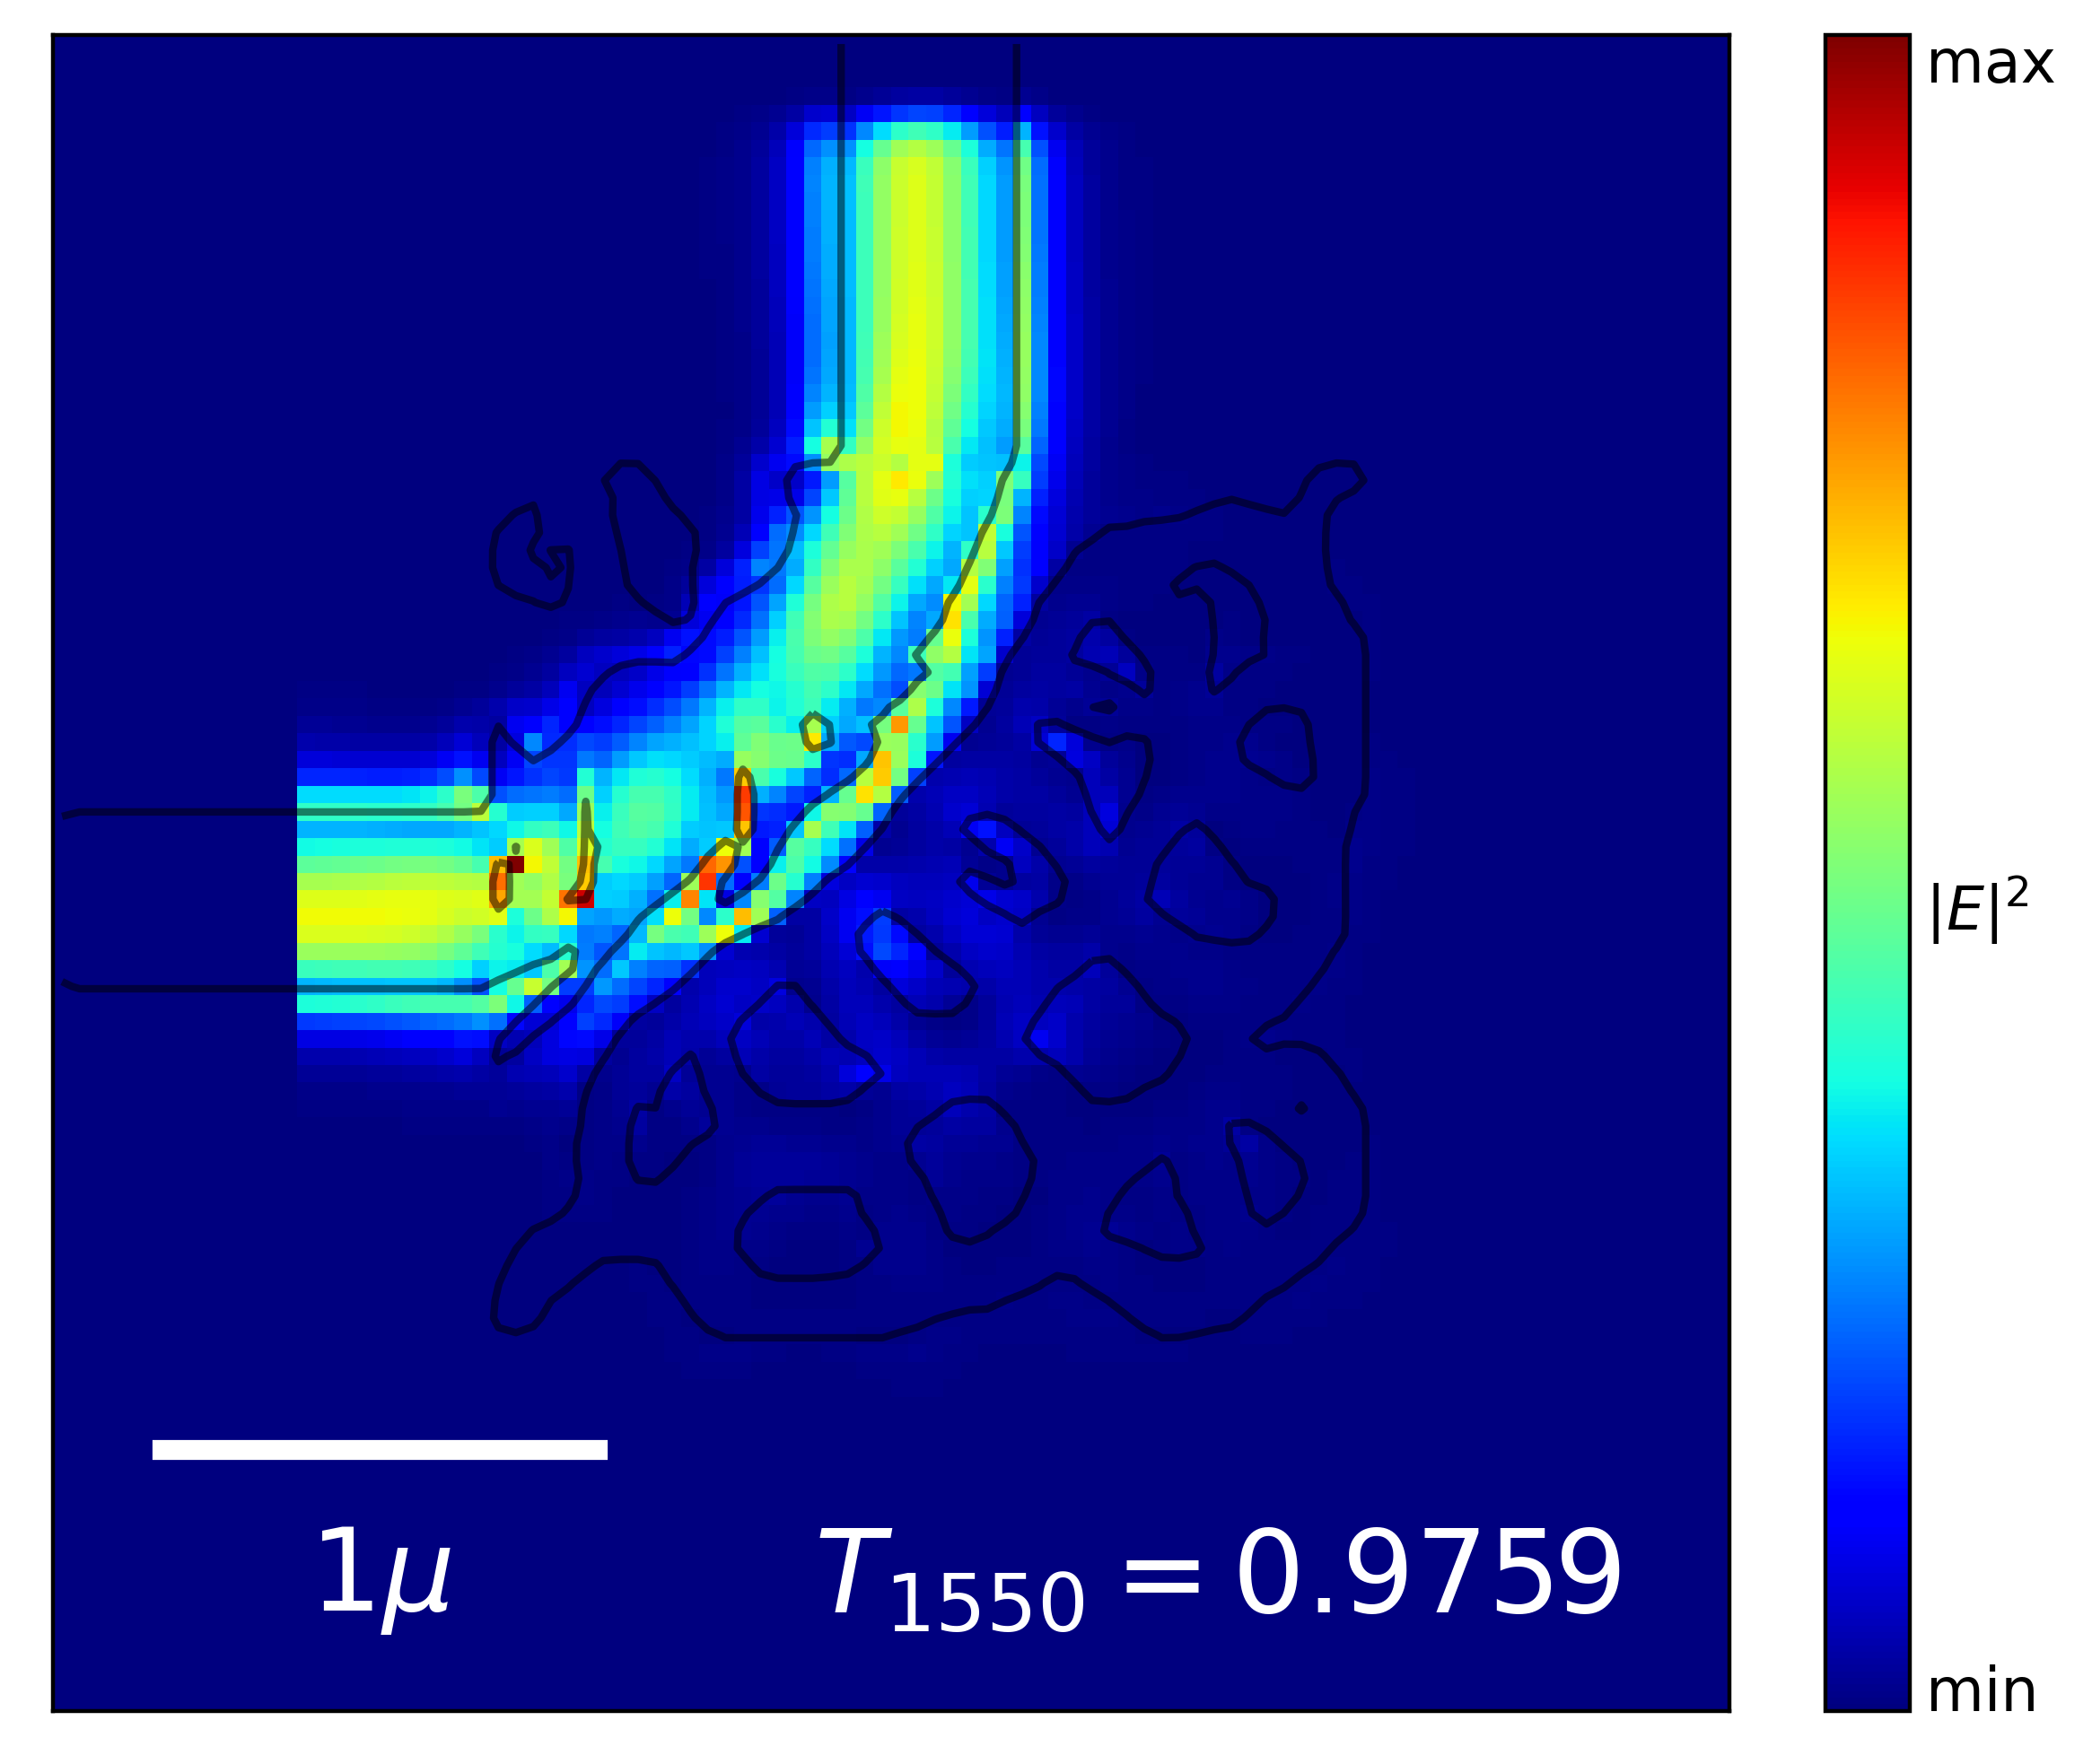
\includegraphics[width=0.33\textwidth]{image/results/bend/L-BFGS-B/visualize_field_cont_128.png} &
      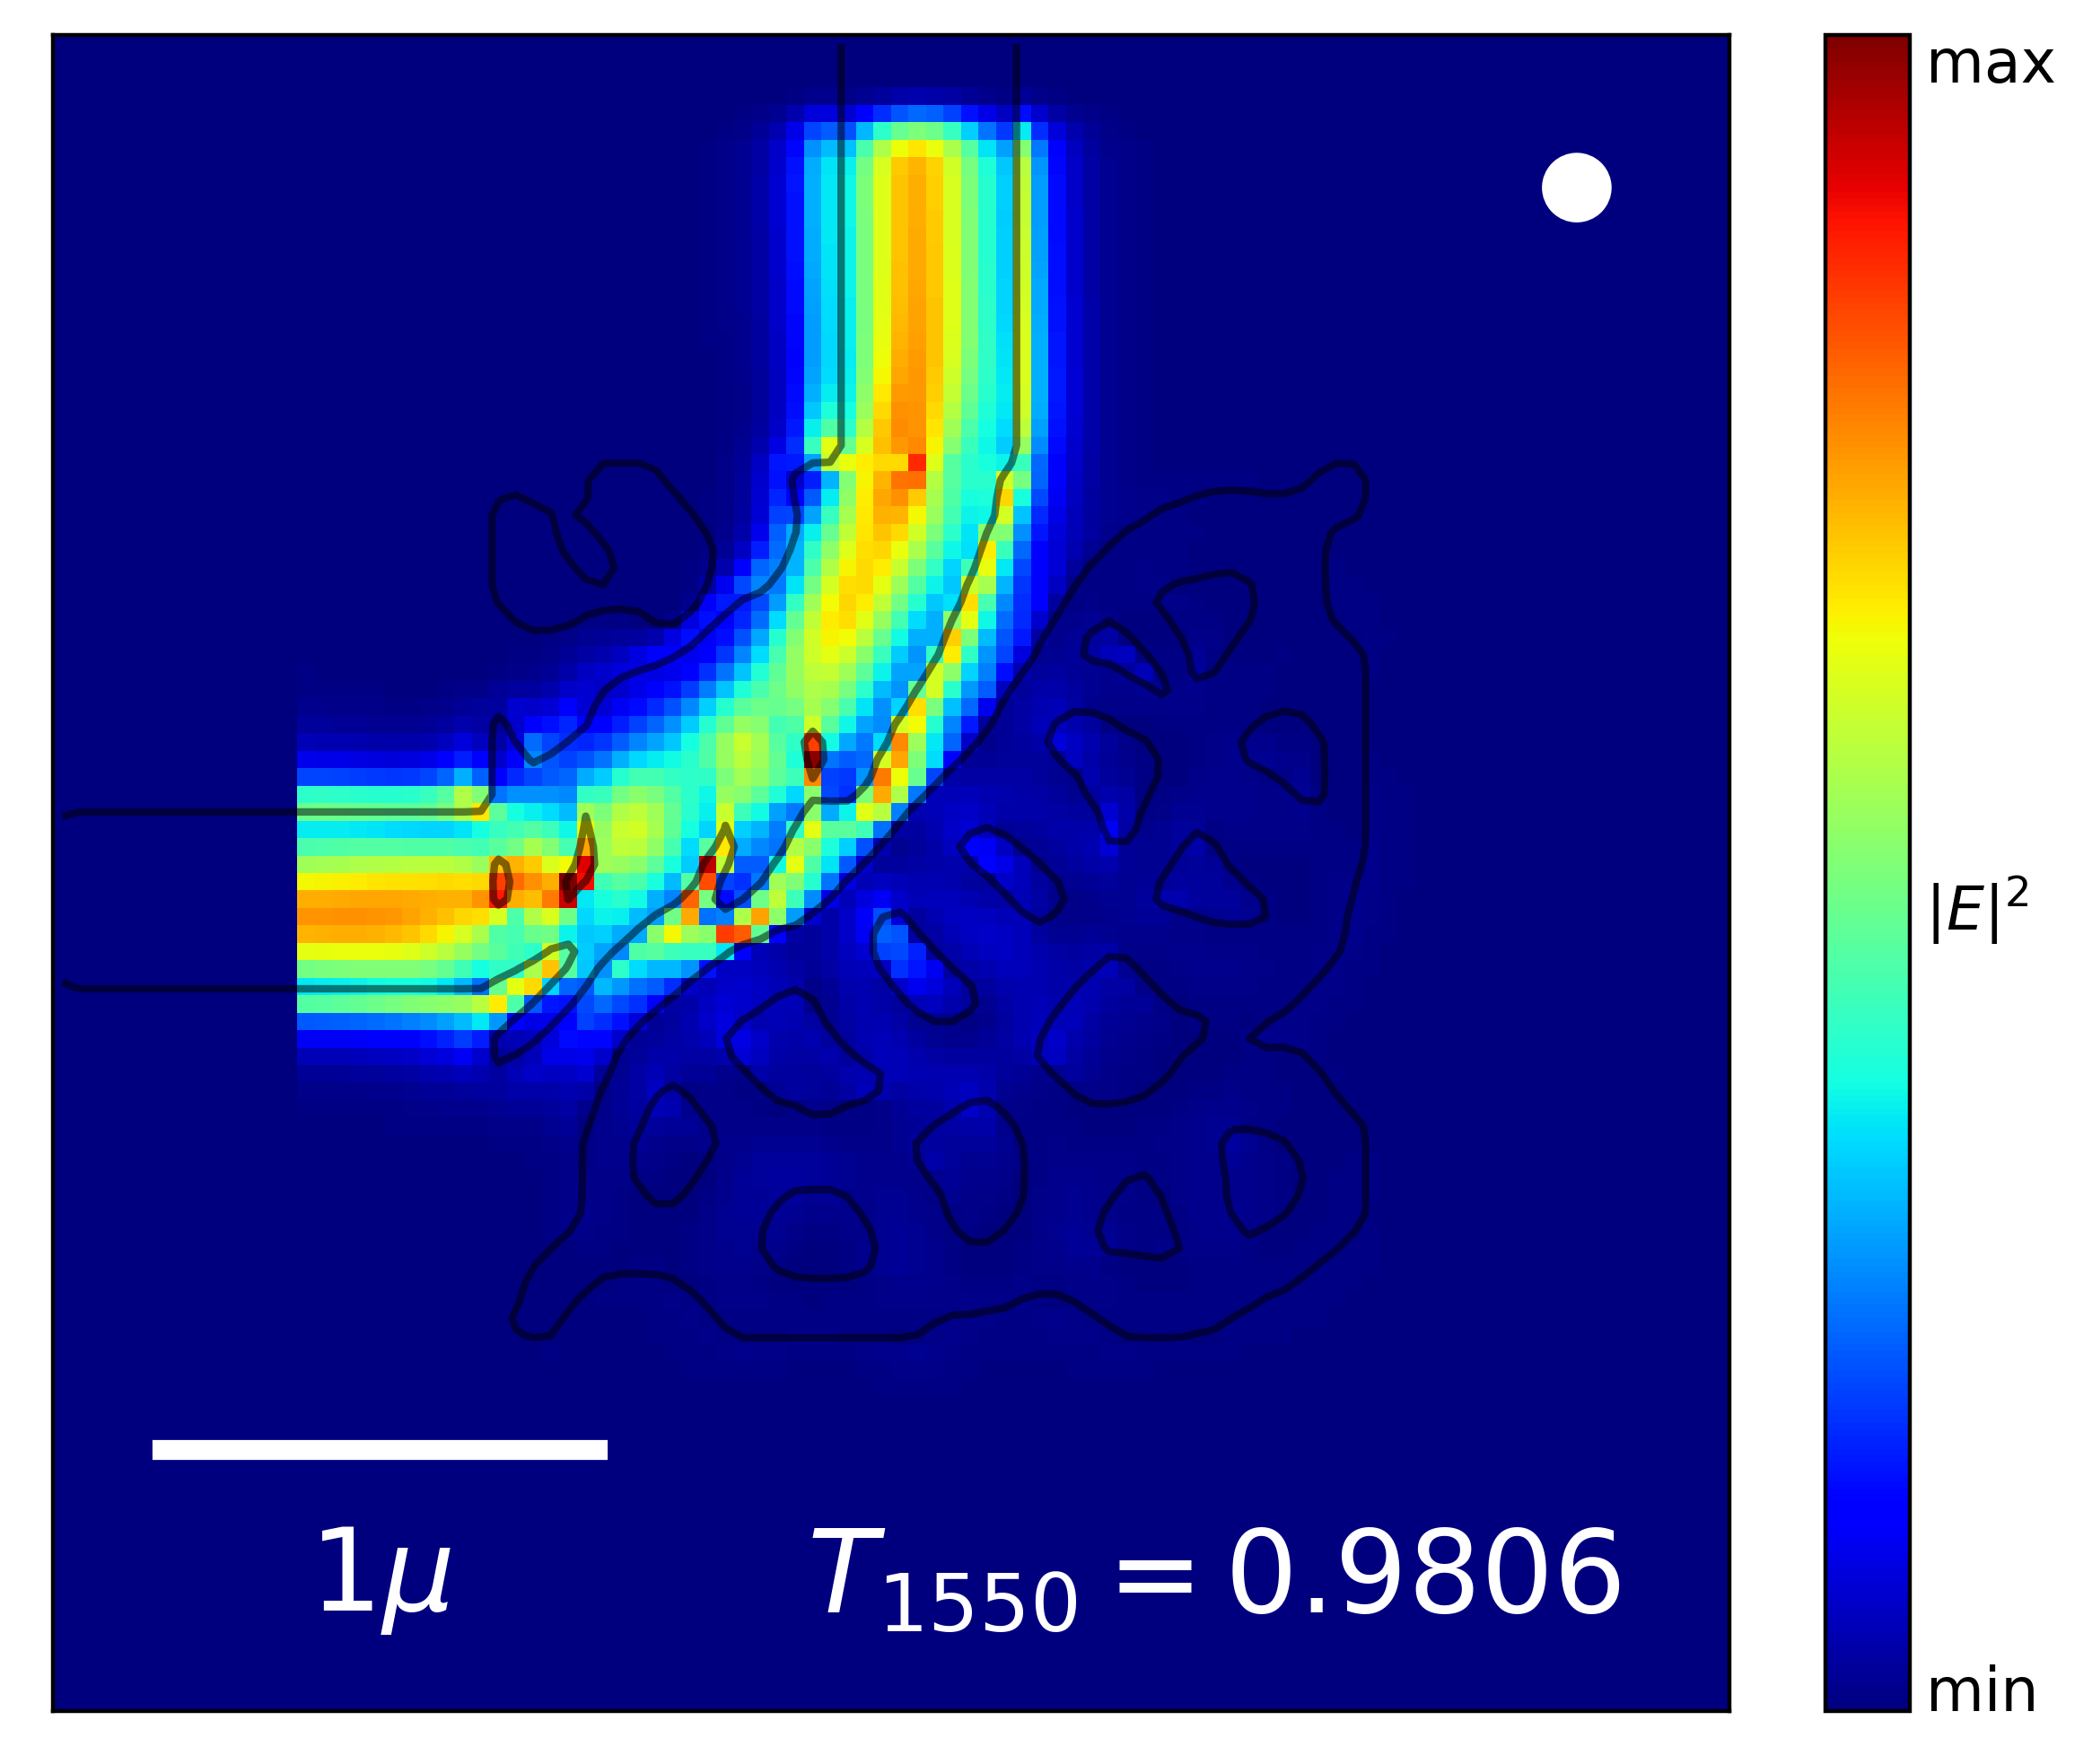
\includegraphics[width=0.33\textwidth]{image/results/bend/L-BFGS-B/visualize_field_disc_128.png} &
      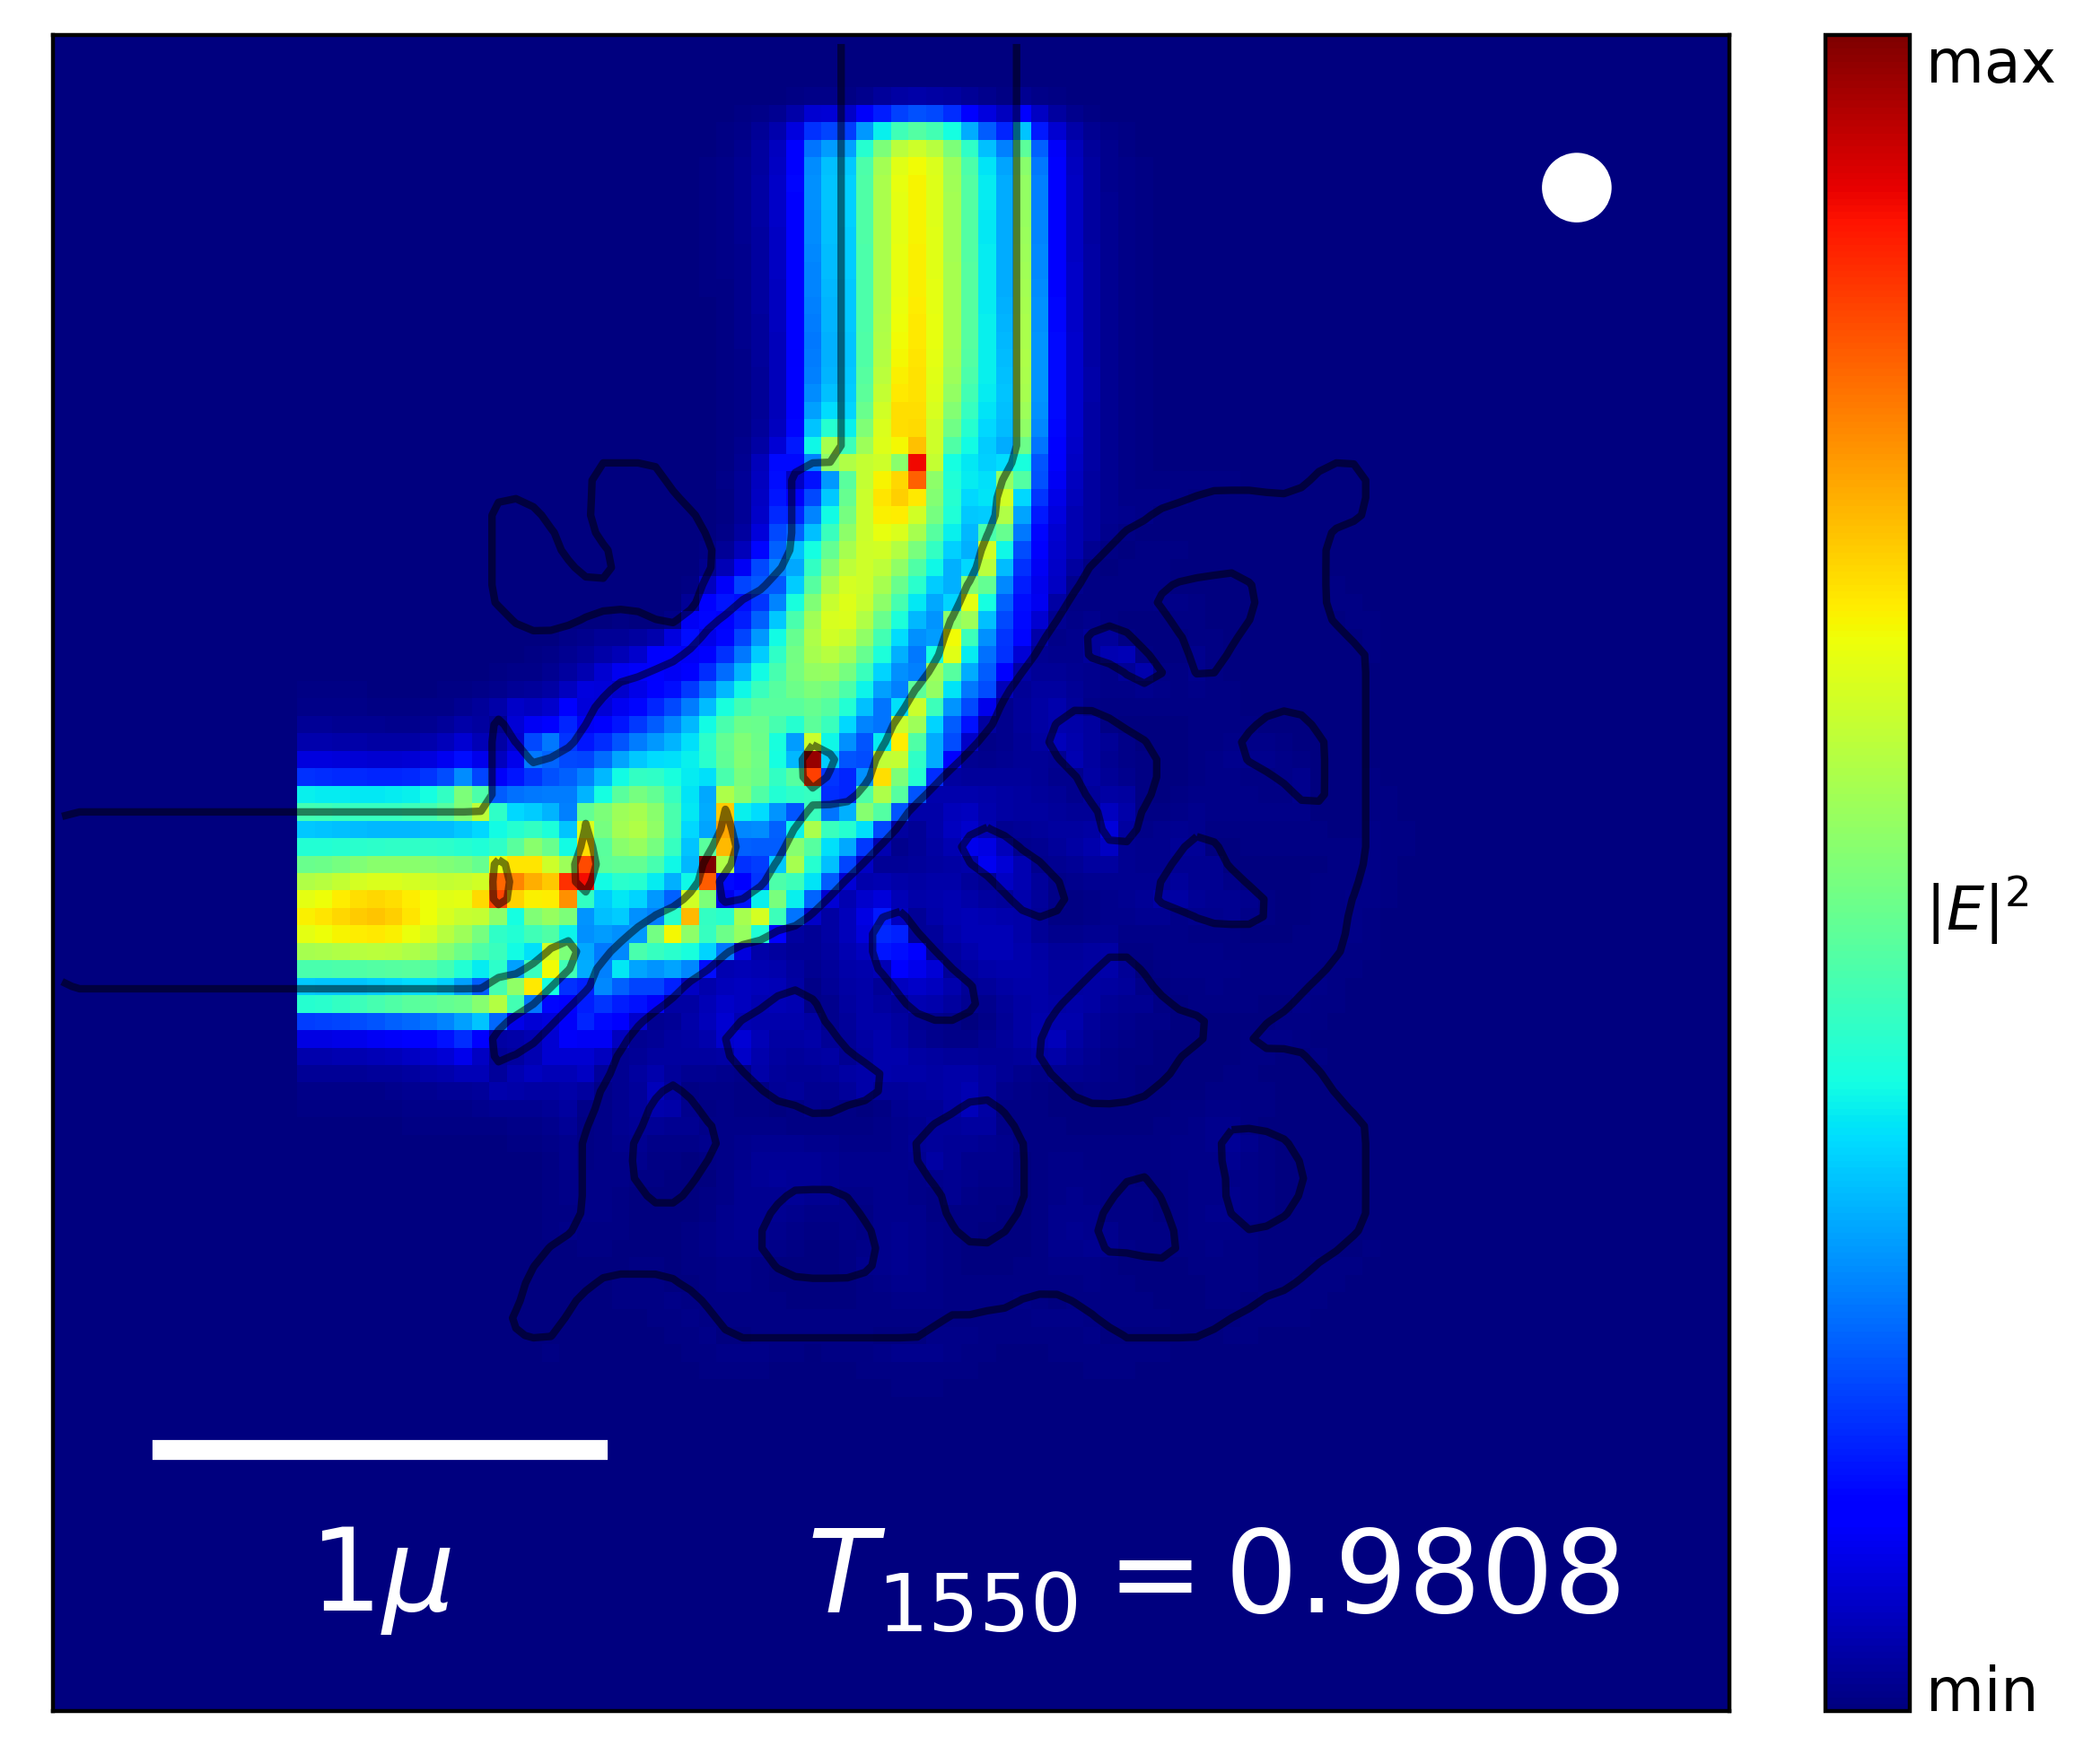
\includegraphics[width=0.33\textwidth]{image/results/bend/L-BFGS-B/visualize_field_fab_128.png} \\
    \hline
      \multirow{2}{*}{256} &
      
\includegraphics[width=0.20\textwidth]{image/results/bend/L-BFGS-B/visualize_eps_cont_256.png} &
      
\includegraphics[width=0.20\textwidth]{image/results/bend/L-BFGS-B/visualize_eps_disc_256.png} &
      
\includegraphics[width=0.20\textwidth]{image/results/bend/L-BFGS-B/visualize_eps_fab_256.png} \\
      \cline{2-4}
      &
      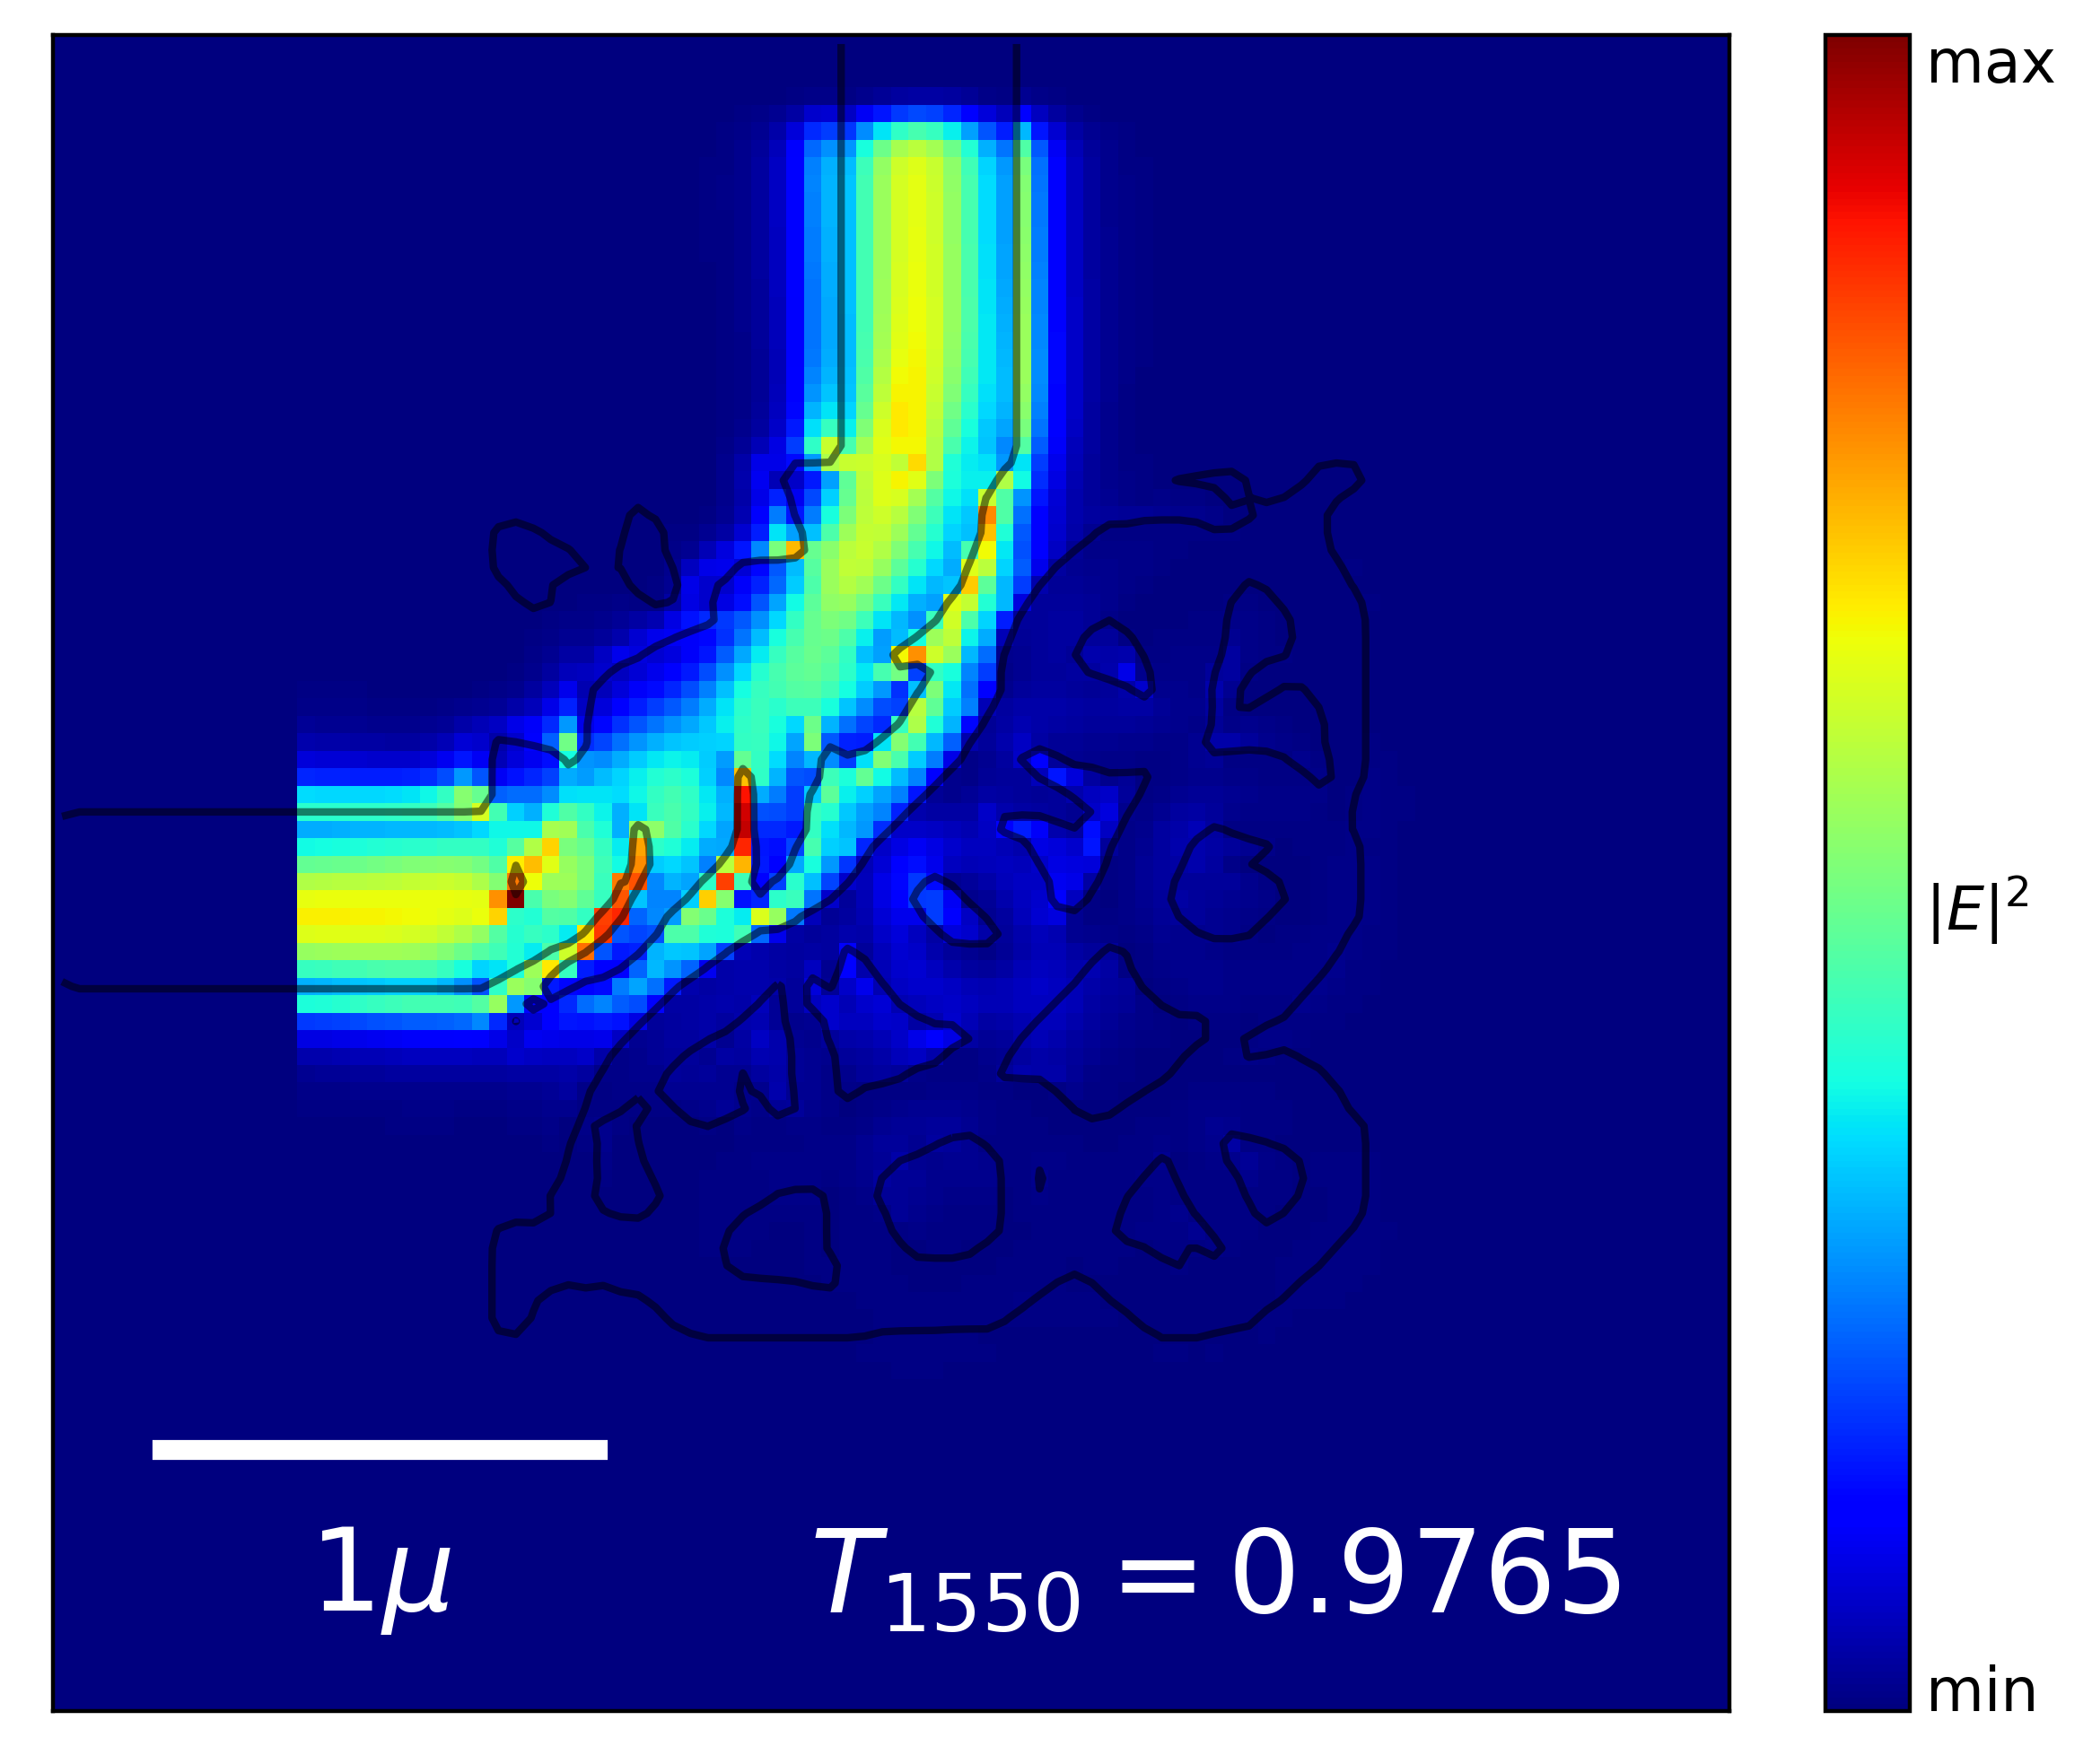
\includegraphics[width=0.33\textwidth]{image/results/bend/L-BFGS-B/visualize_field_cont_256.png} &
      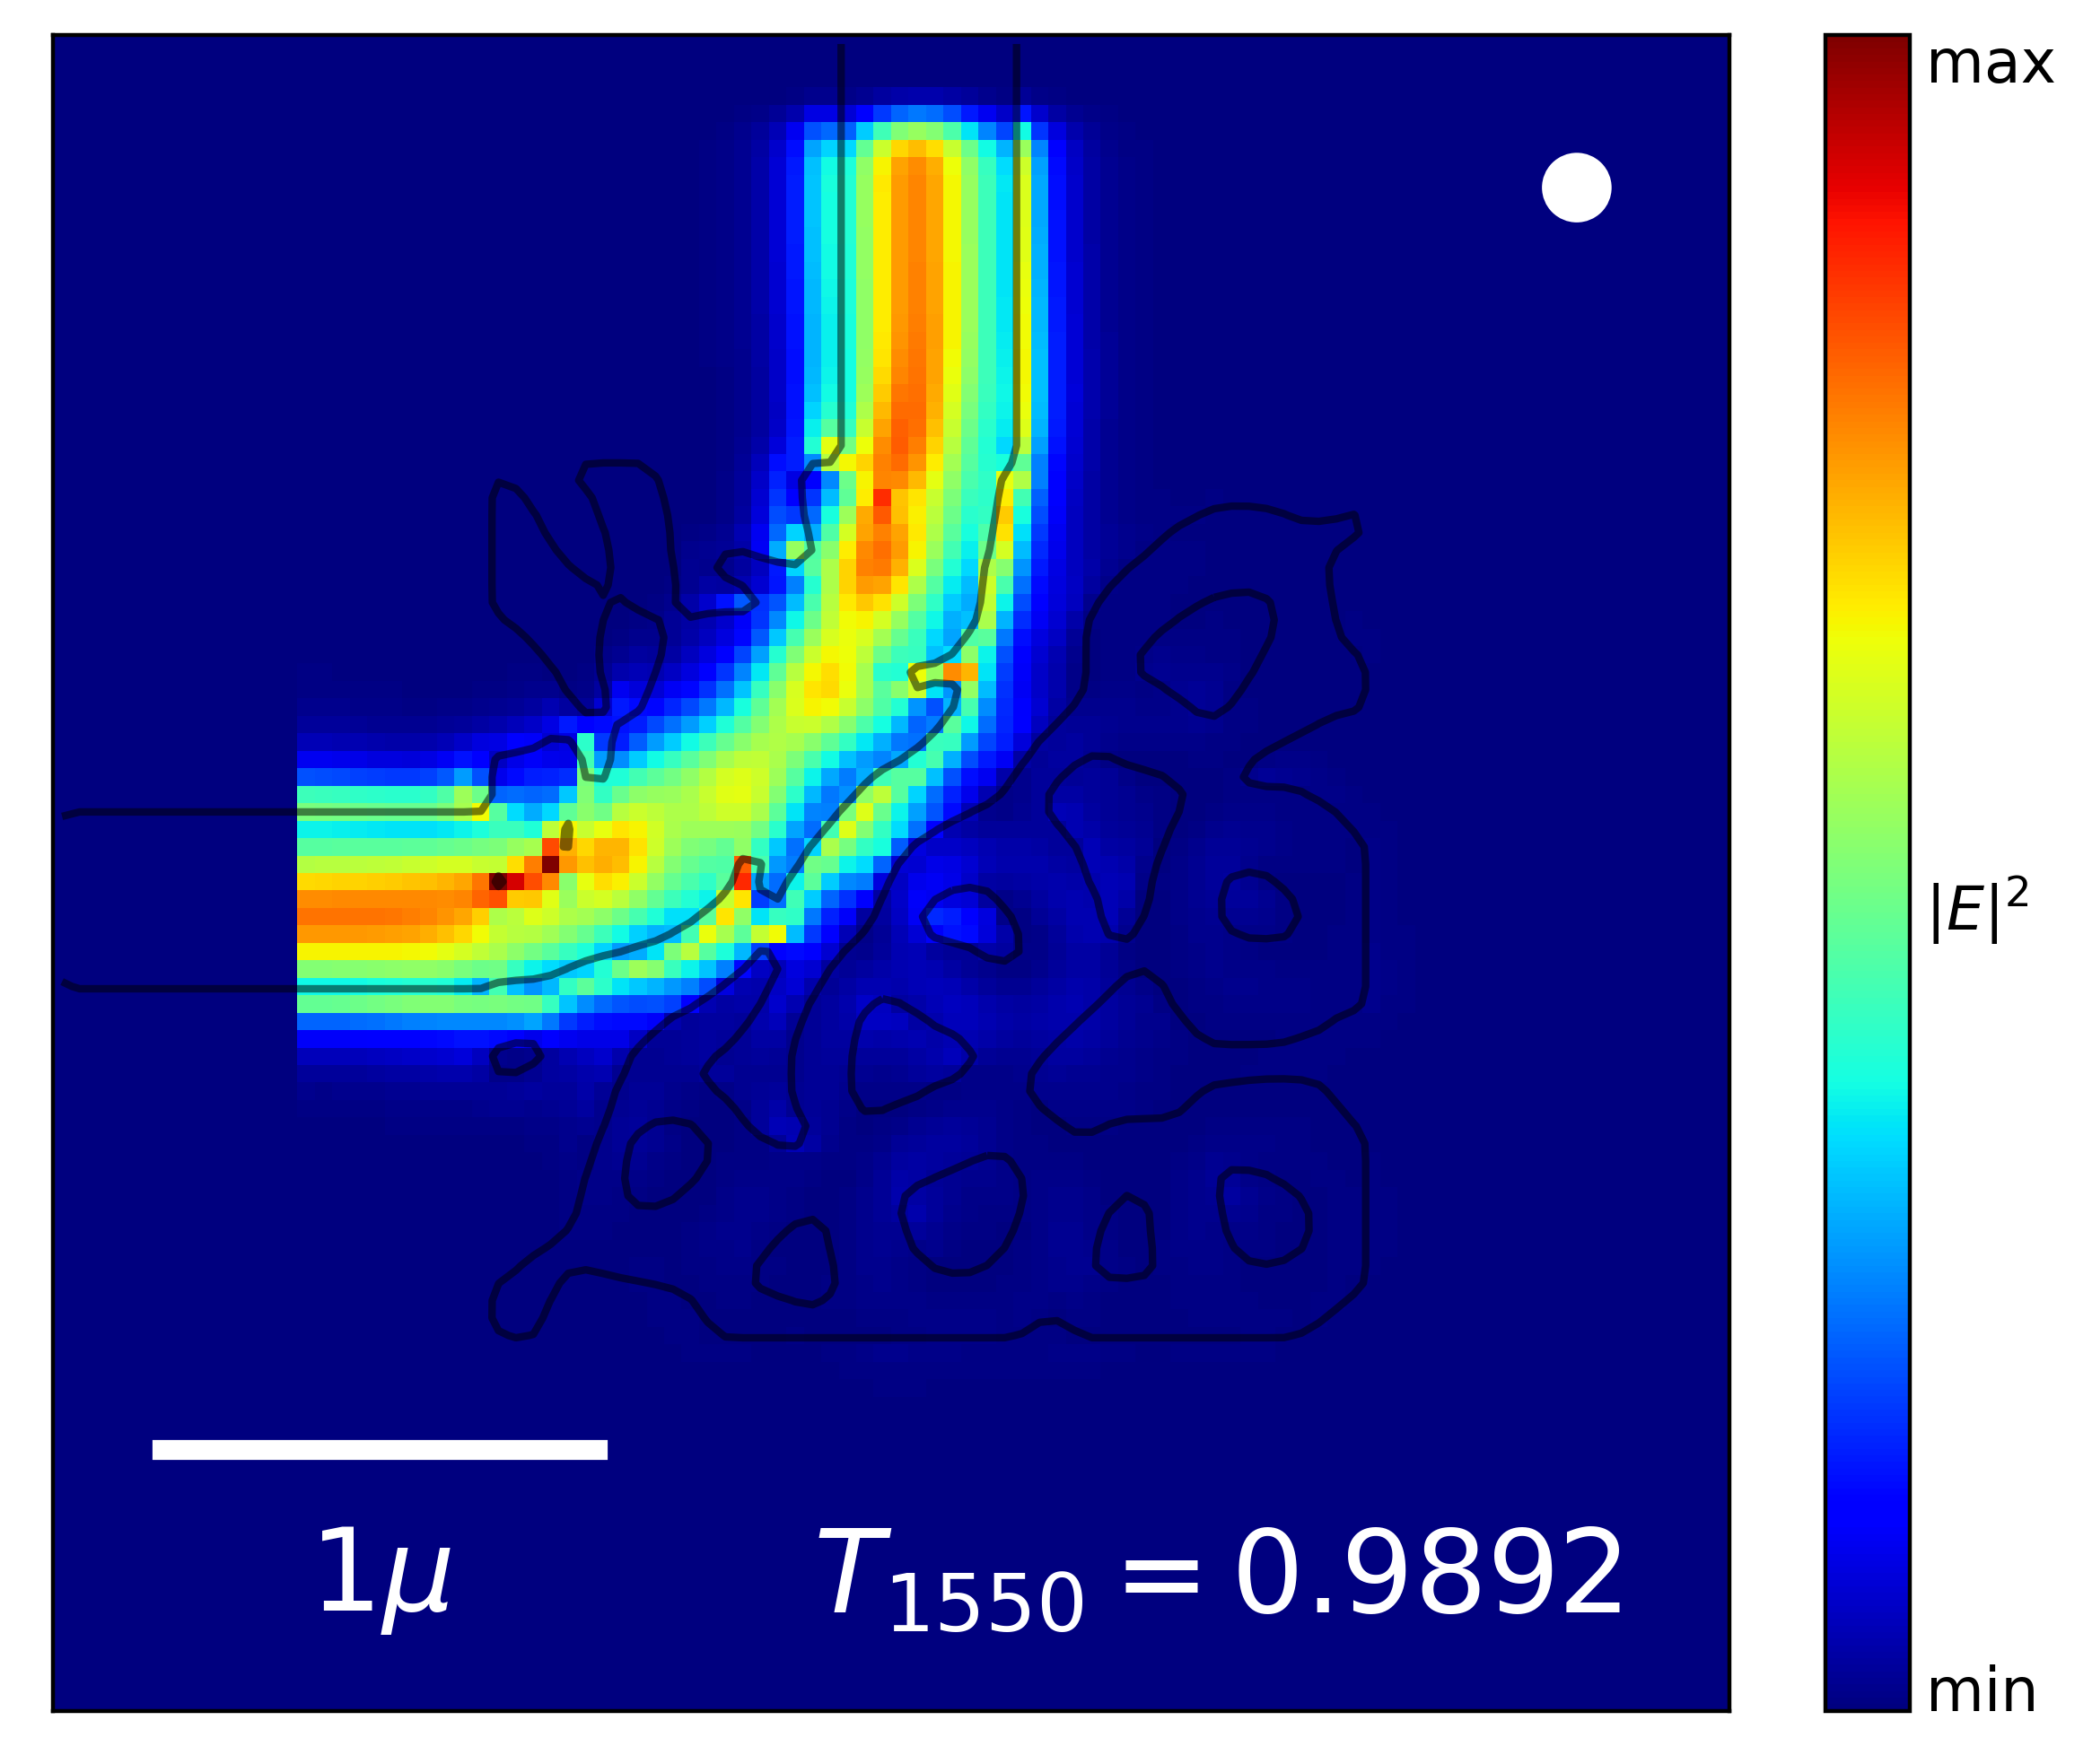
\includegraphics[width=0.33\textwidth]{image/results/bend/L-BFGS-B/visualize_field_disc_256.png} &
      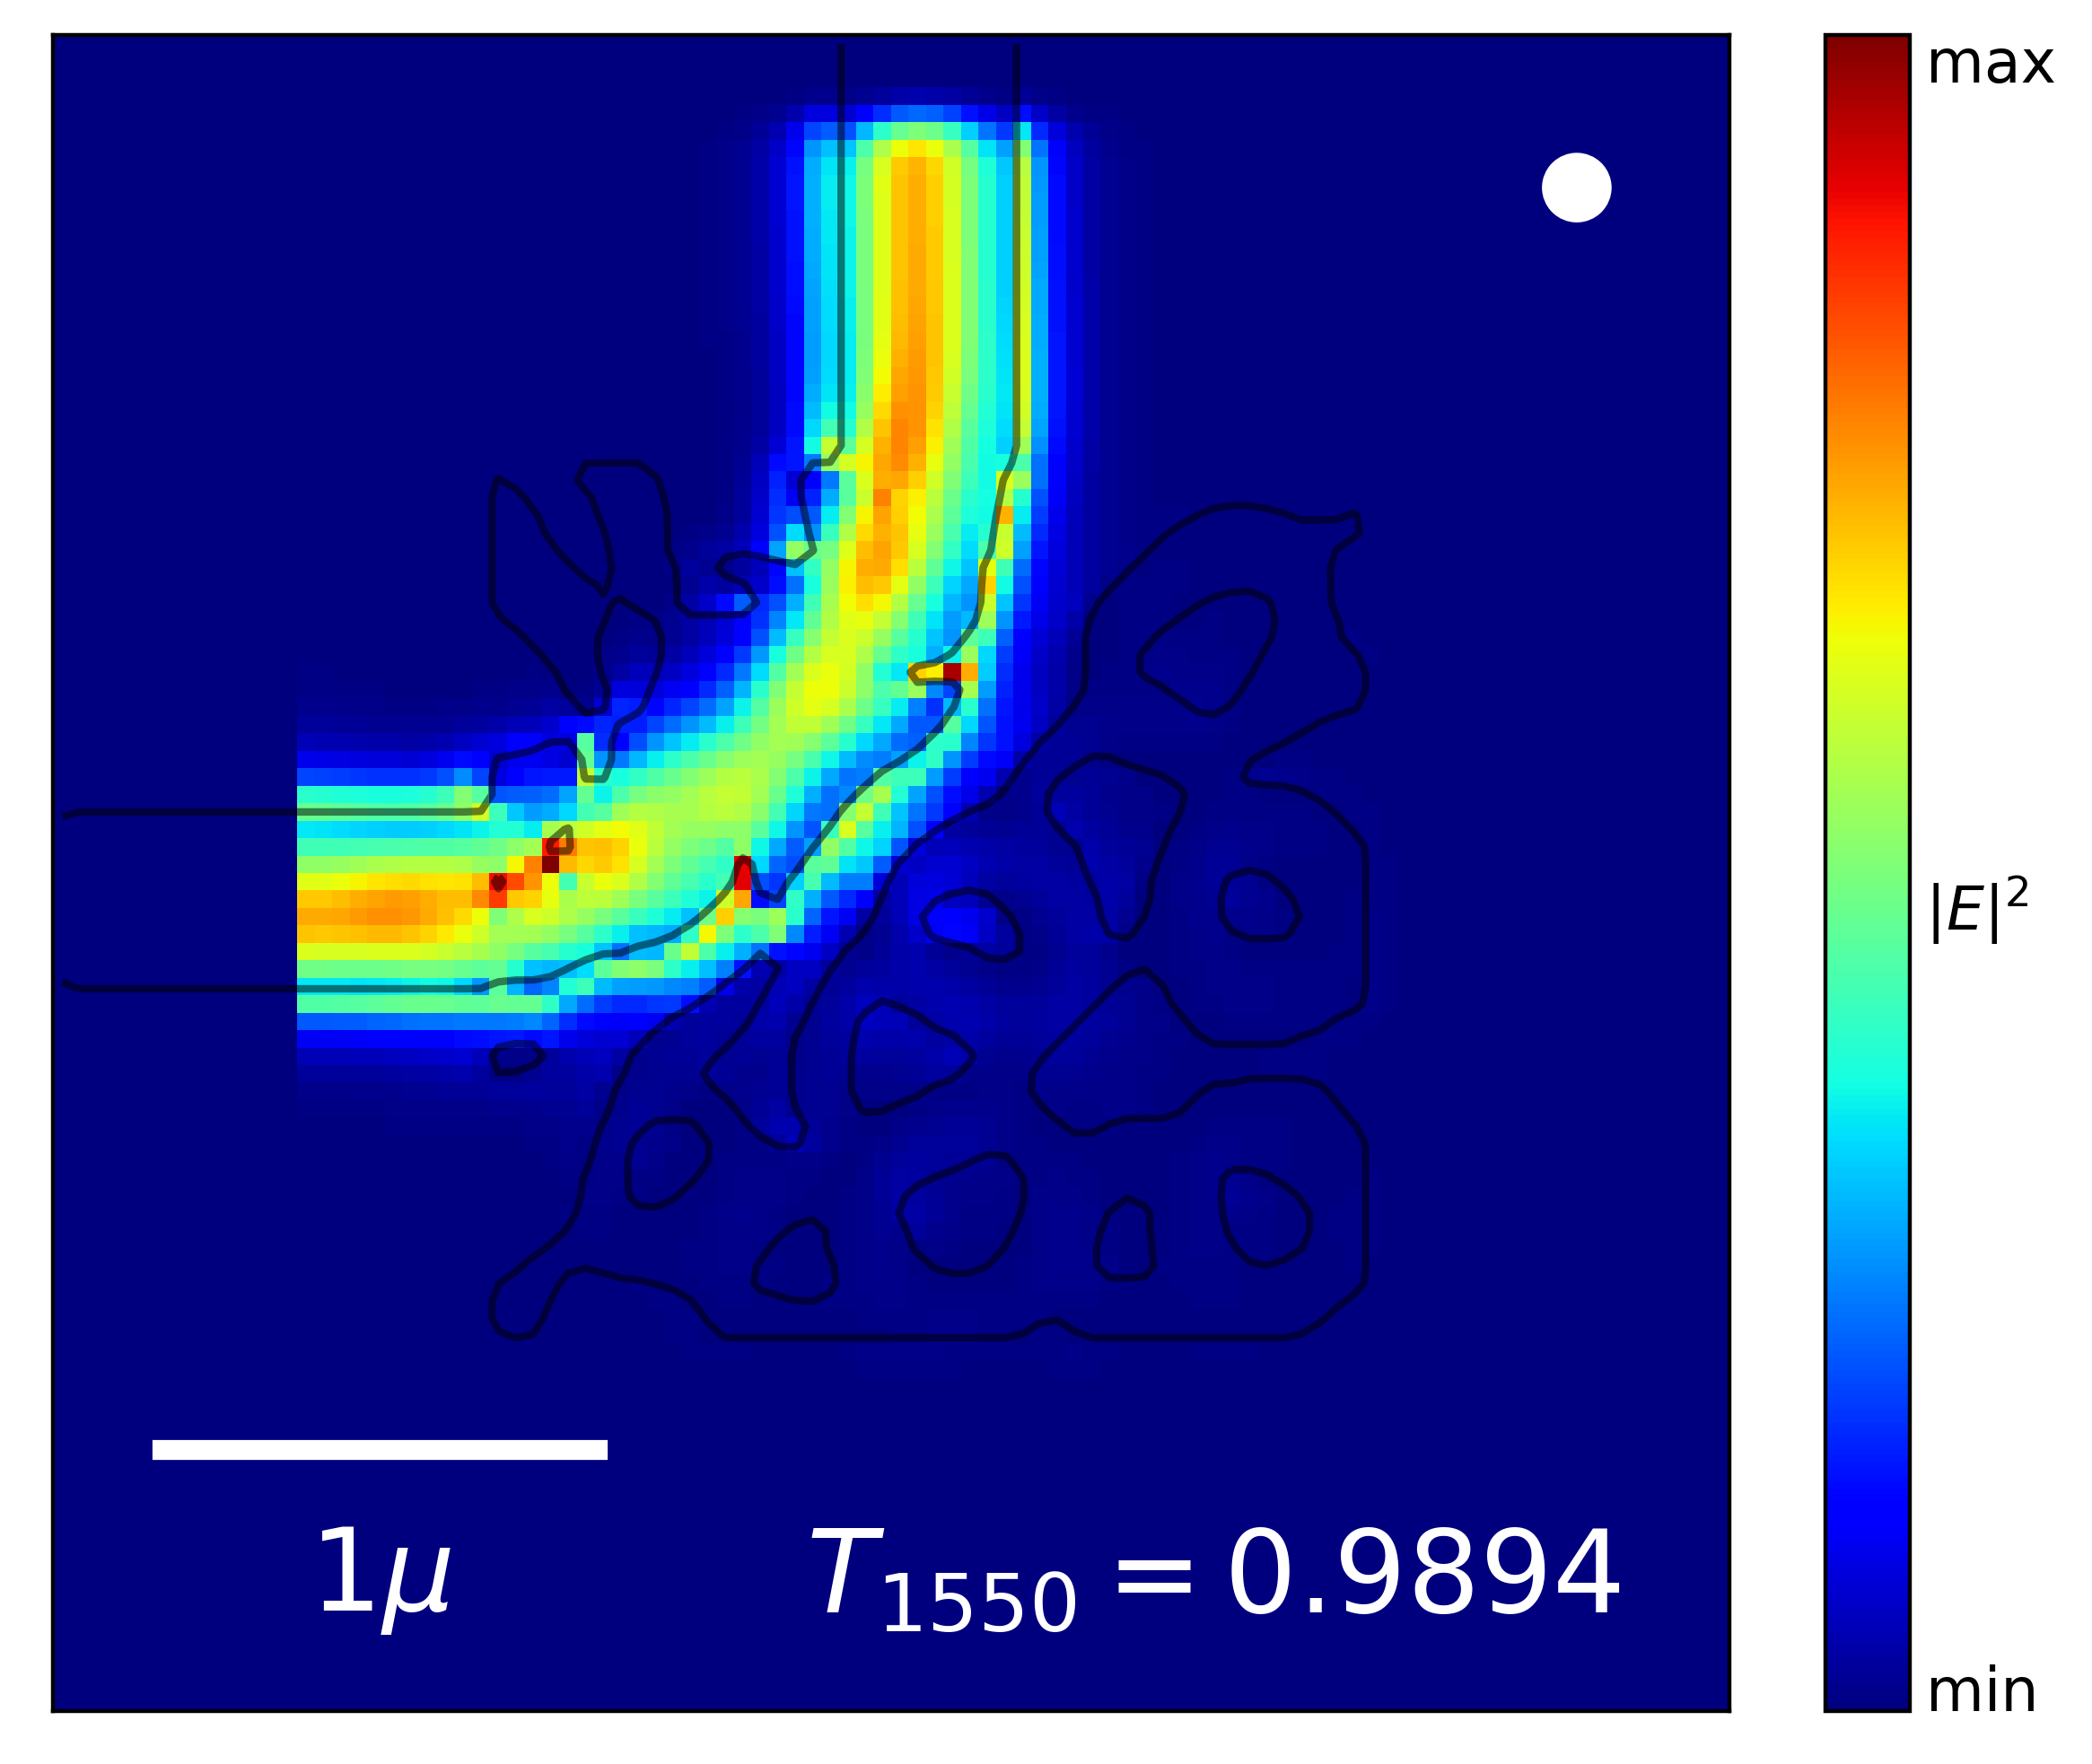
\includegraphics[width=0.33\textwidth]{image/results/bend/L-BFGS-B/visualize_field_fab_256.png} \\
    \hline
      \multirow{2}{*}{512} &
      
\includegraphics[width=0.20\textwidth]{image/results/bend/L-BFGS-B/visualize_eps_cont_512.png} &
      
\includegraphics[width=0.20\textwidth]{image/results/bend/L-BFGS-B/visualize_eps_disc_512.png} &
      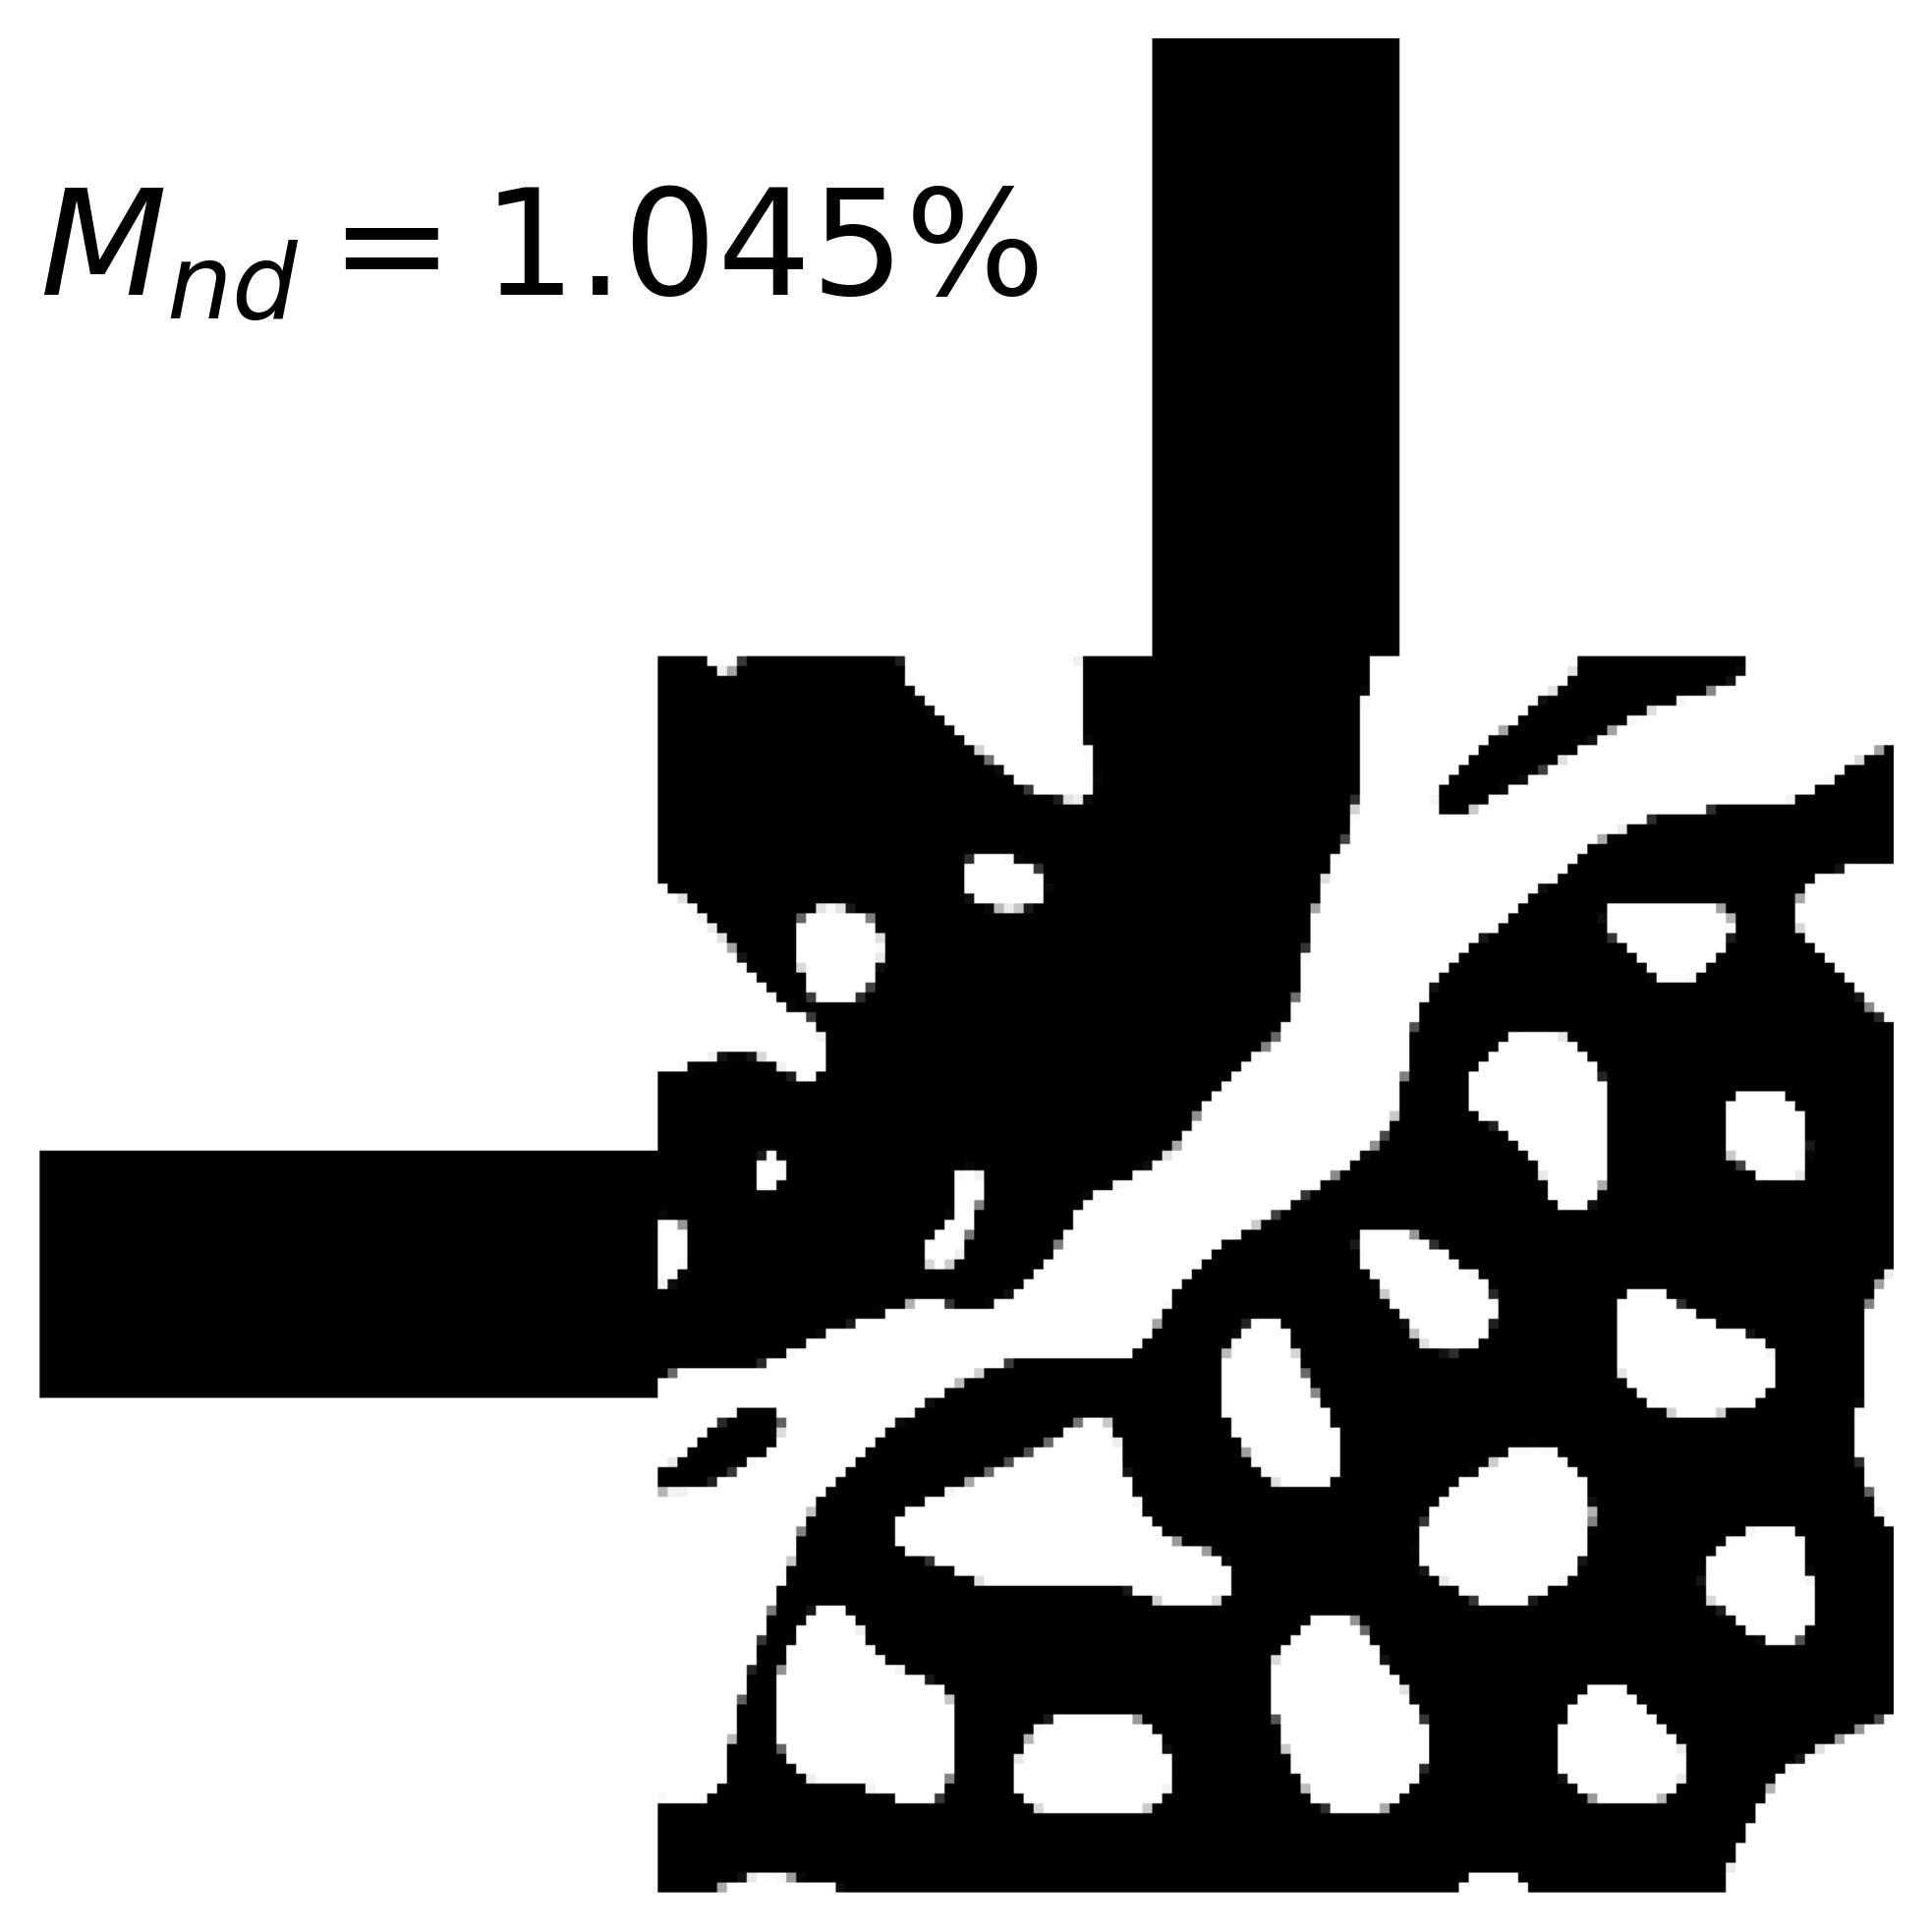
\includegraphics[width=0.20\textwidth]{image/results/bend/L-BFGS-B/visualize_eps_fab_512.png} \\
      \cline{2-4}
      &
      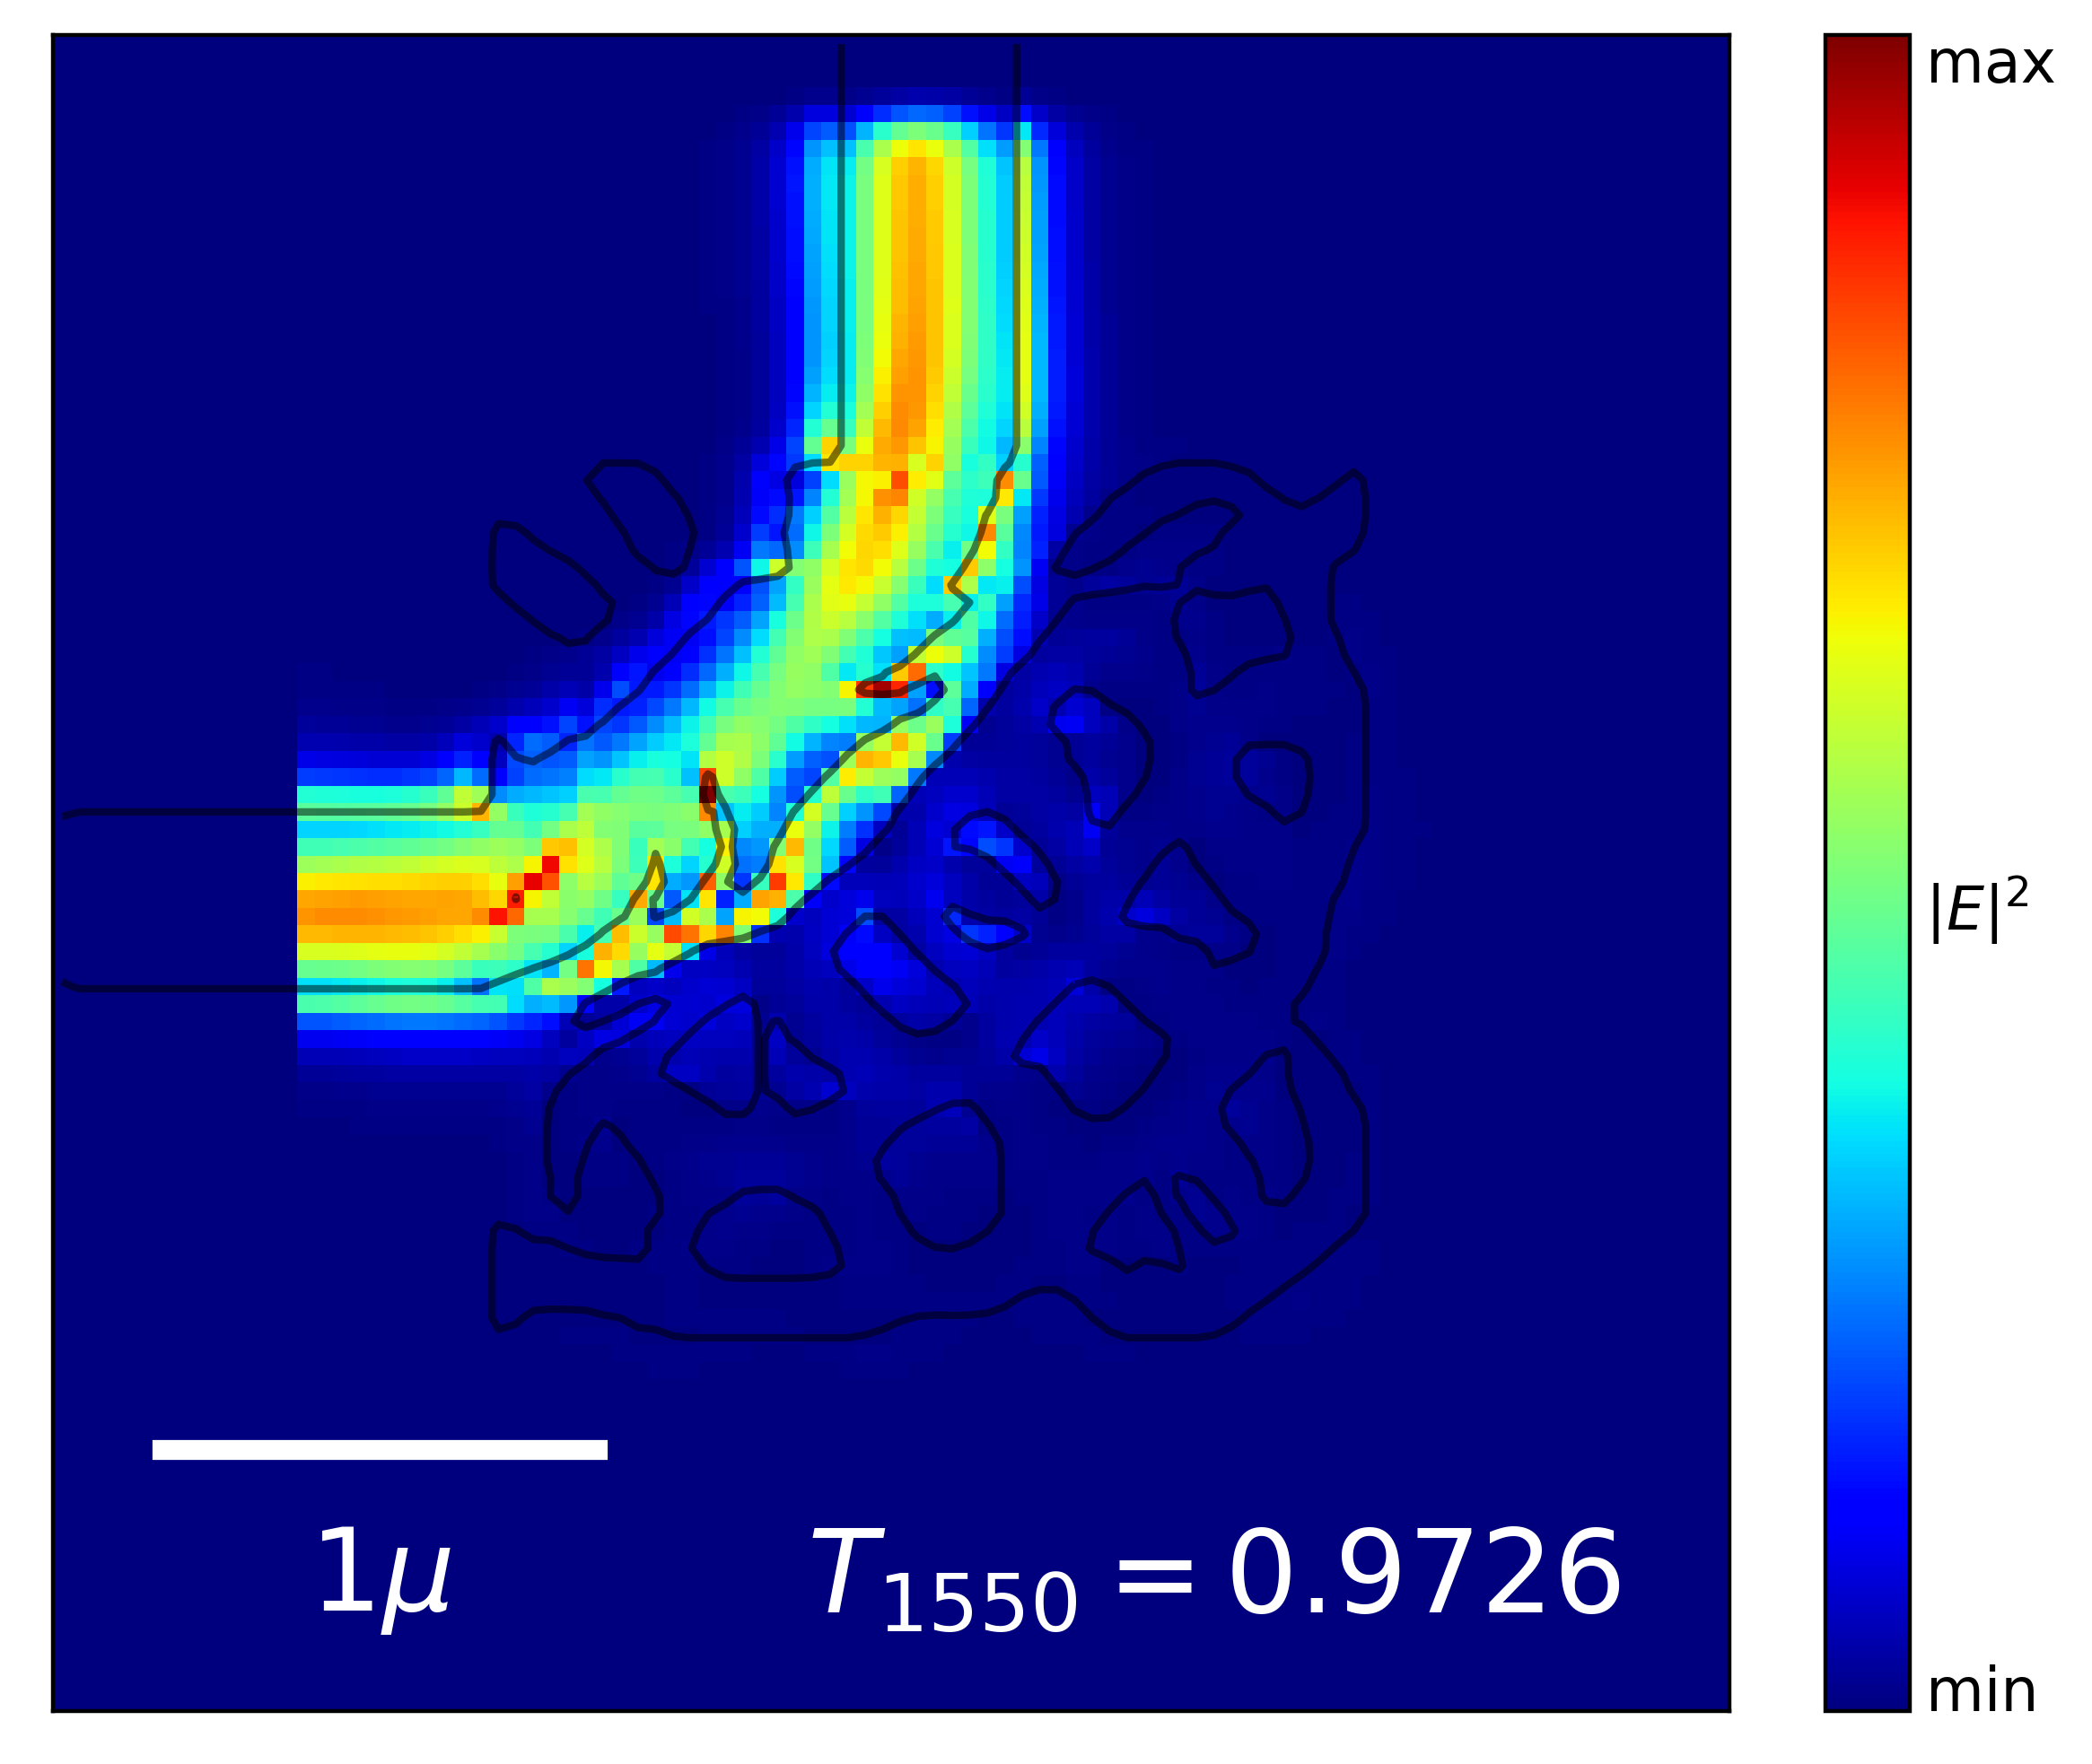
\includegraphics[width=0.33\textwidth]{image/results/bend/L-BFGS-B/visualize_field_cont_512.png} &
      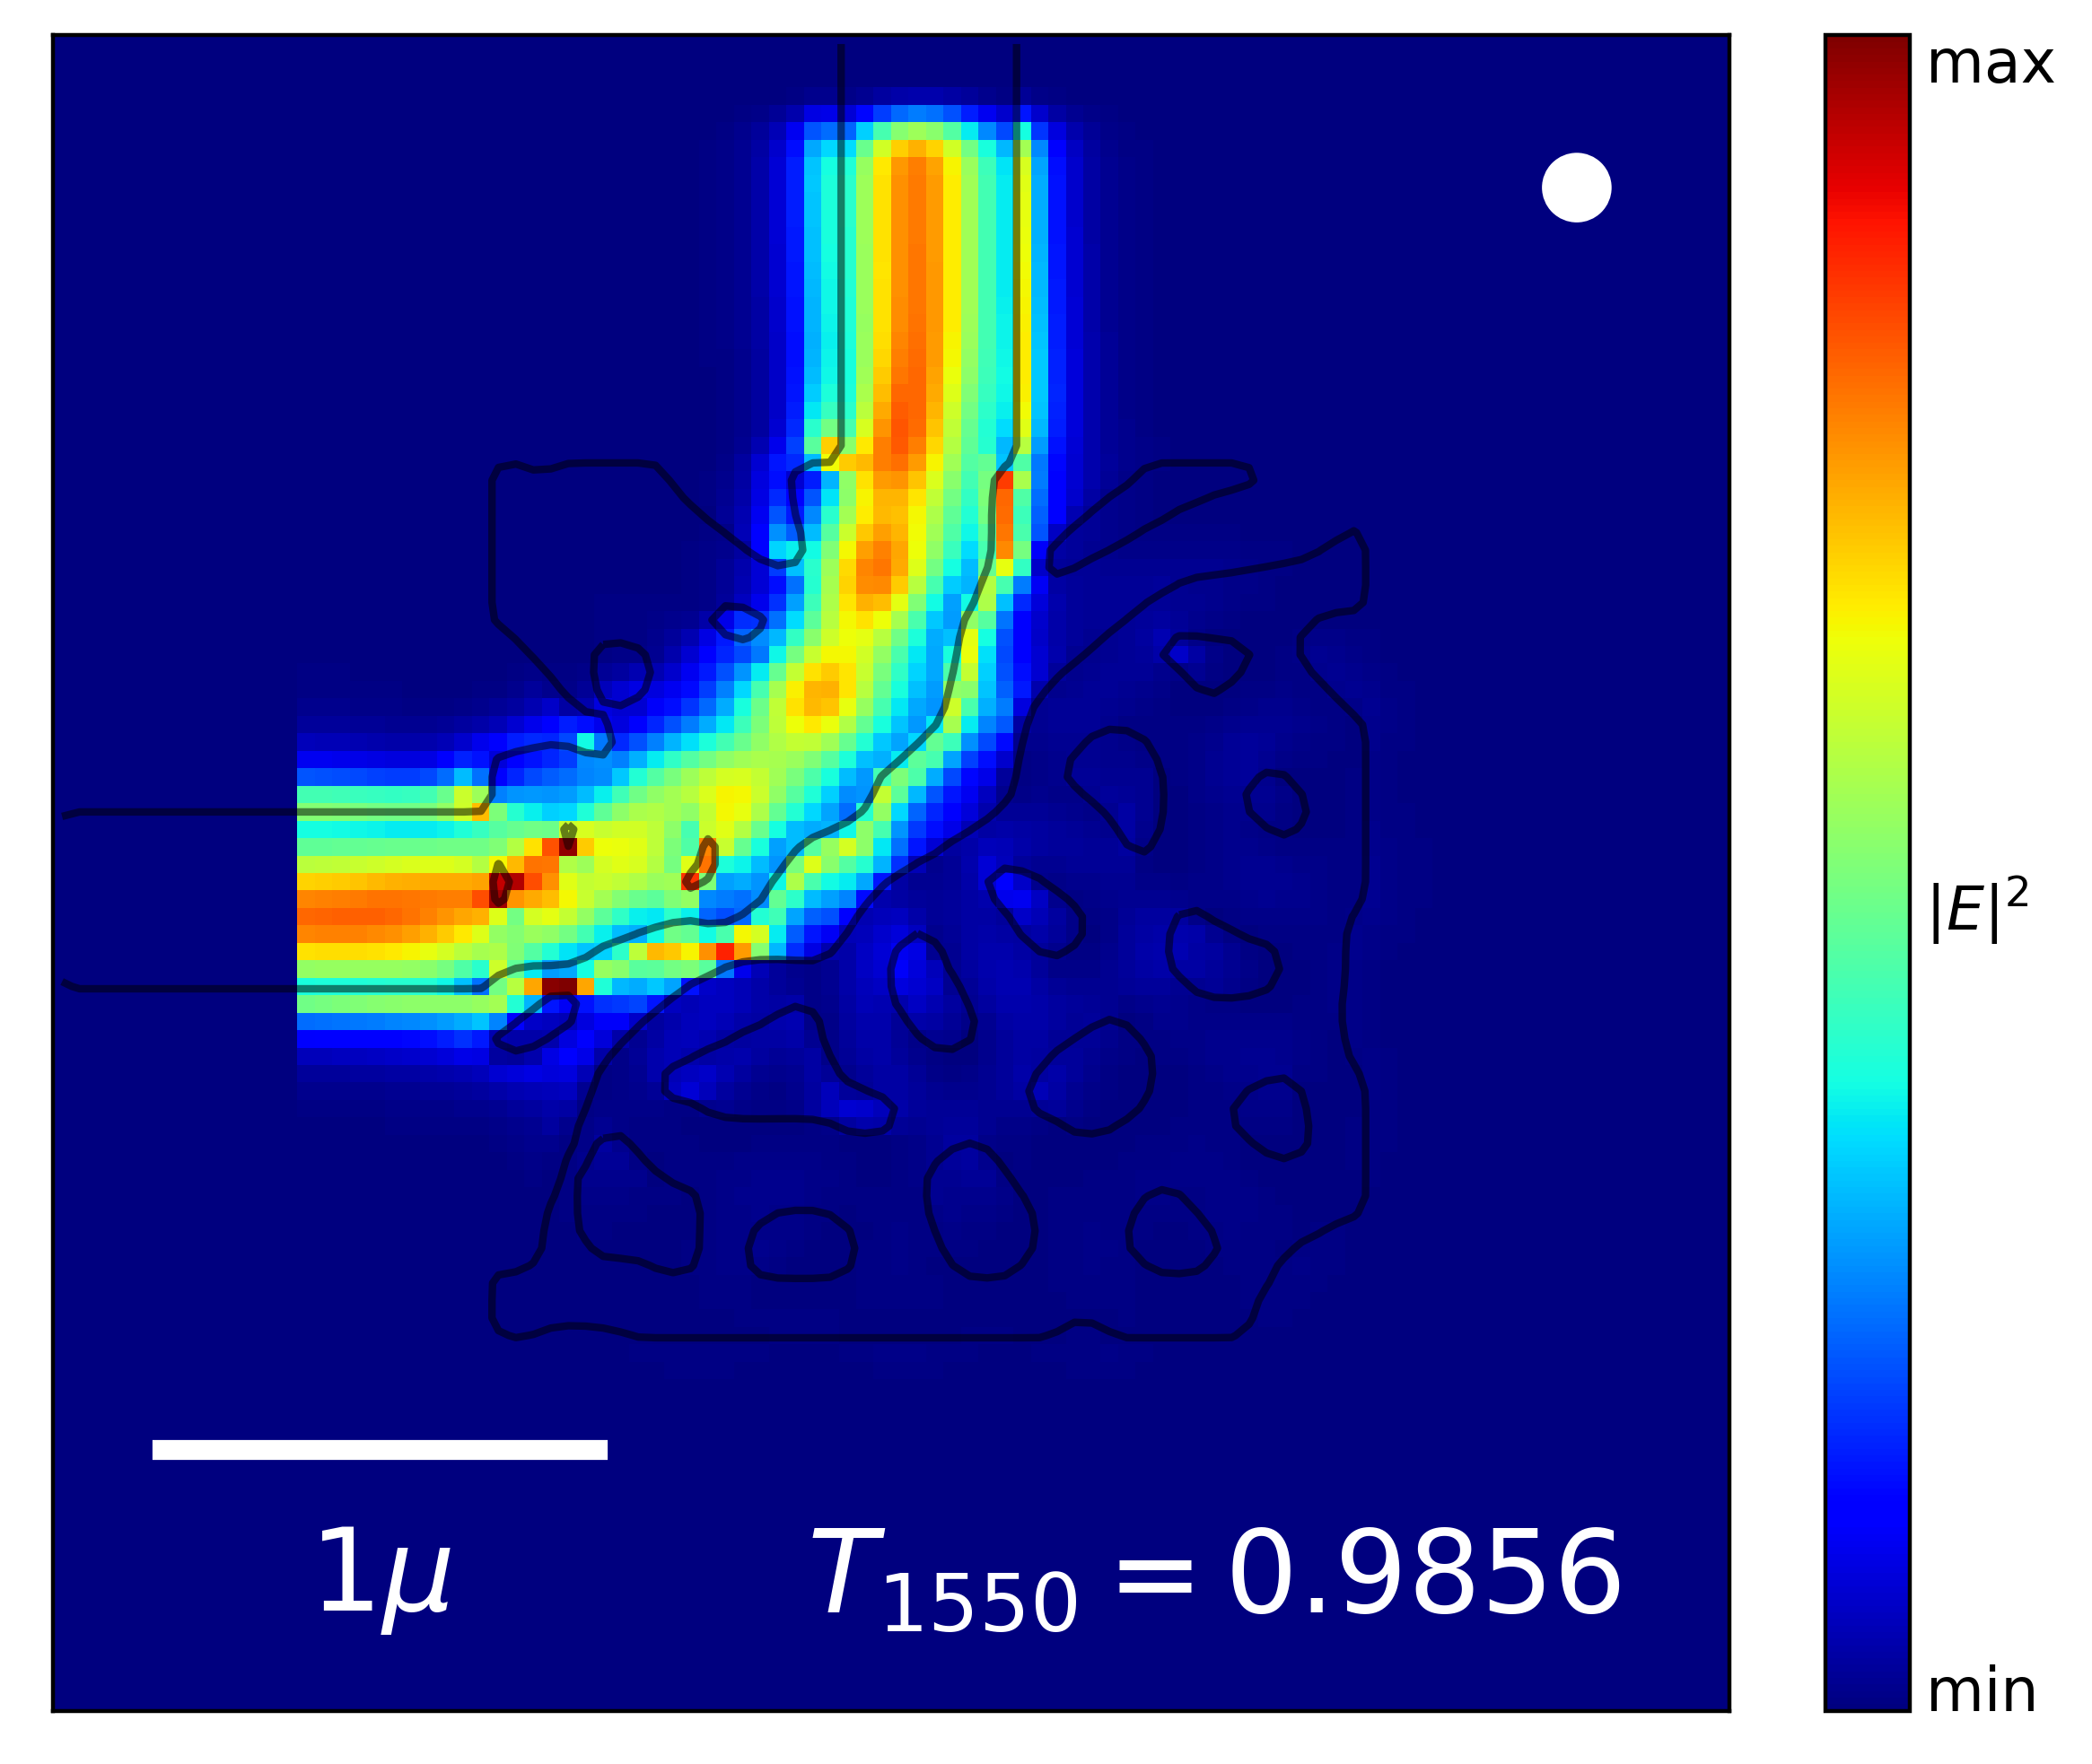
\includegraphics[width=0.33\textwidth]{image/results/bend/L-BFGS-B/visualize_field_disc_512.png} &
      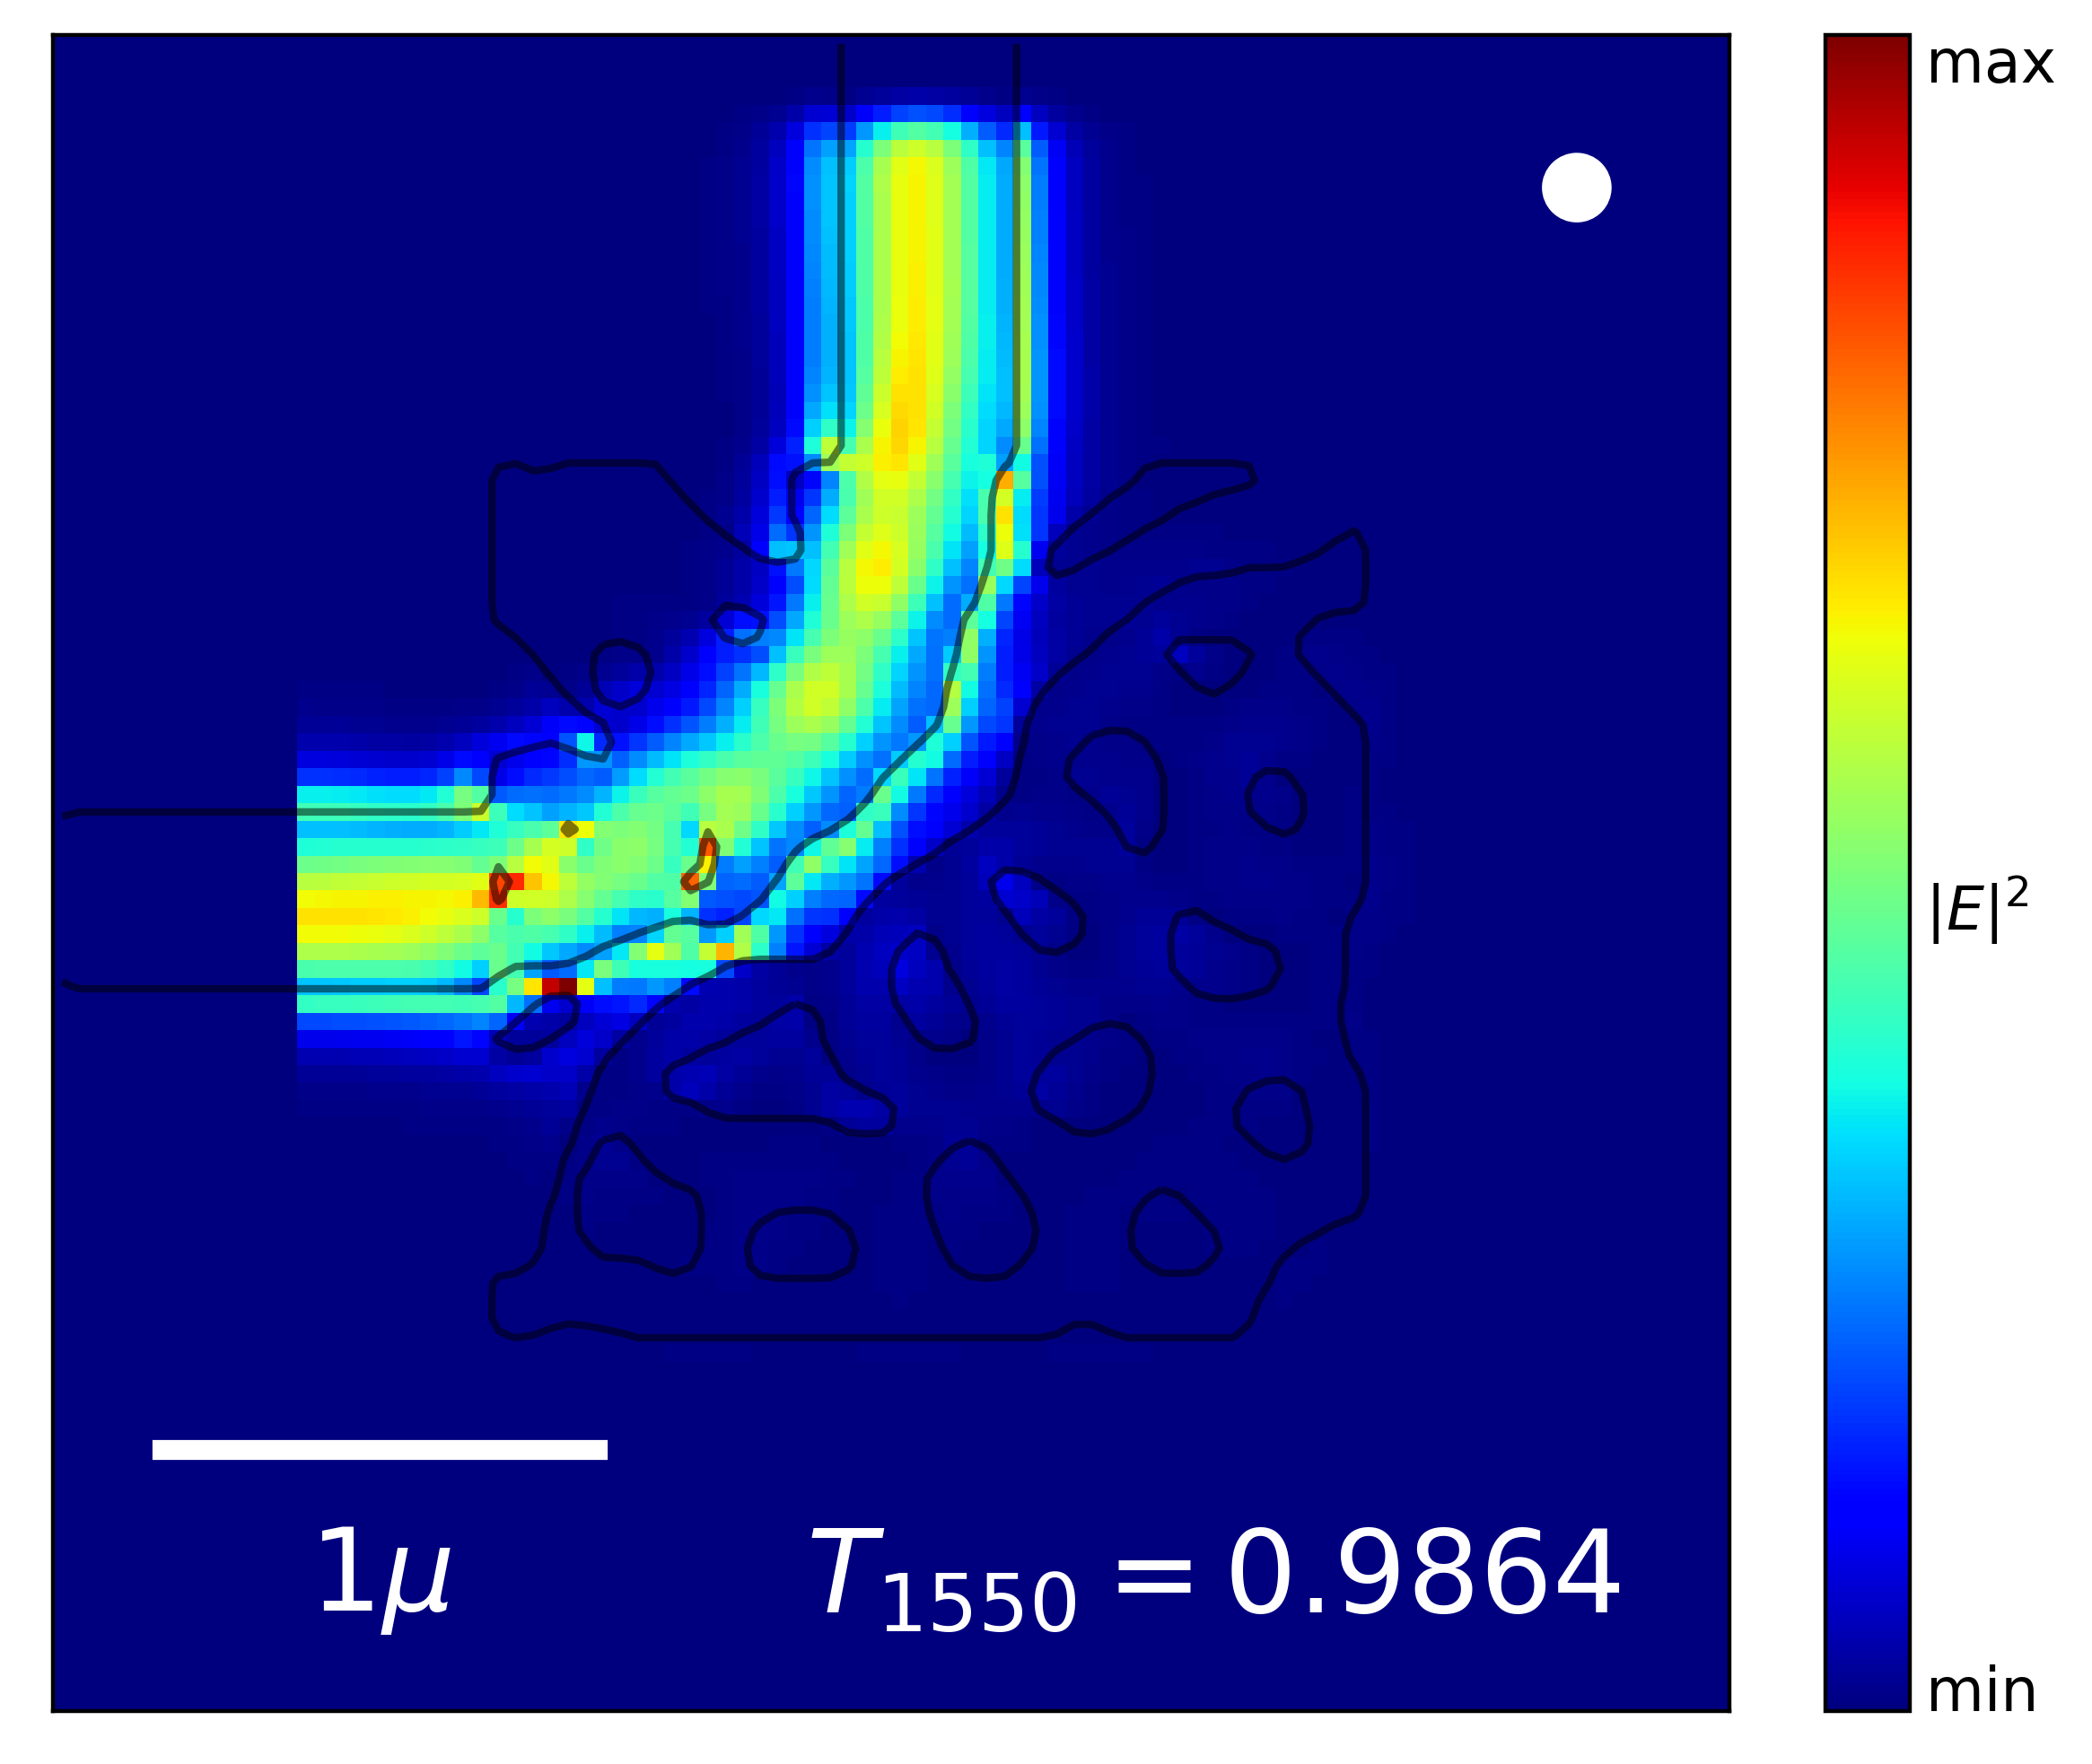
\includegraphics[width=0.33\textwidth]{image/results/bend/L-BFGS-B/visualize_field_fab_512.png} \\
    \hline
    \end{tabular}
    \hspace*{-3cm}
    \caption{Resultados de la optimización continua al optimizar el \emph{bend} usando L-BFGS-B}
    \label{tab:opt-cont-L-BFGS-B-bend}
\end{table}

% WDM - L-BFGS-B
\begin{landscape}
\begin{table}[ht]
    \centering
    \vspace*{-2.5cm}
    \hspace*{-5cm}
    \begin{tabular}{|c|c|c|c|}
    \hline 
    \emph{Seed} & Opt. continua & Opt. discreta &  Opt. de fabricación \\
    \hline
      \multirow{2}{*}{128} &
      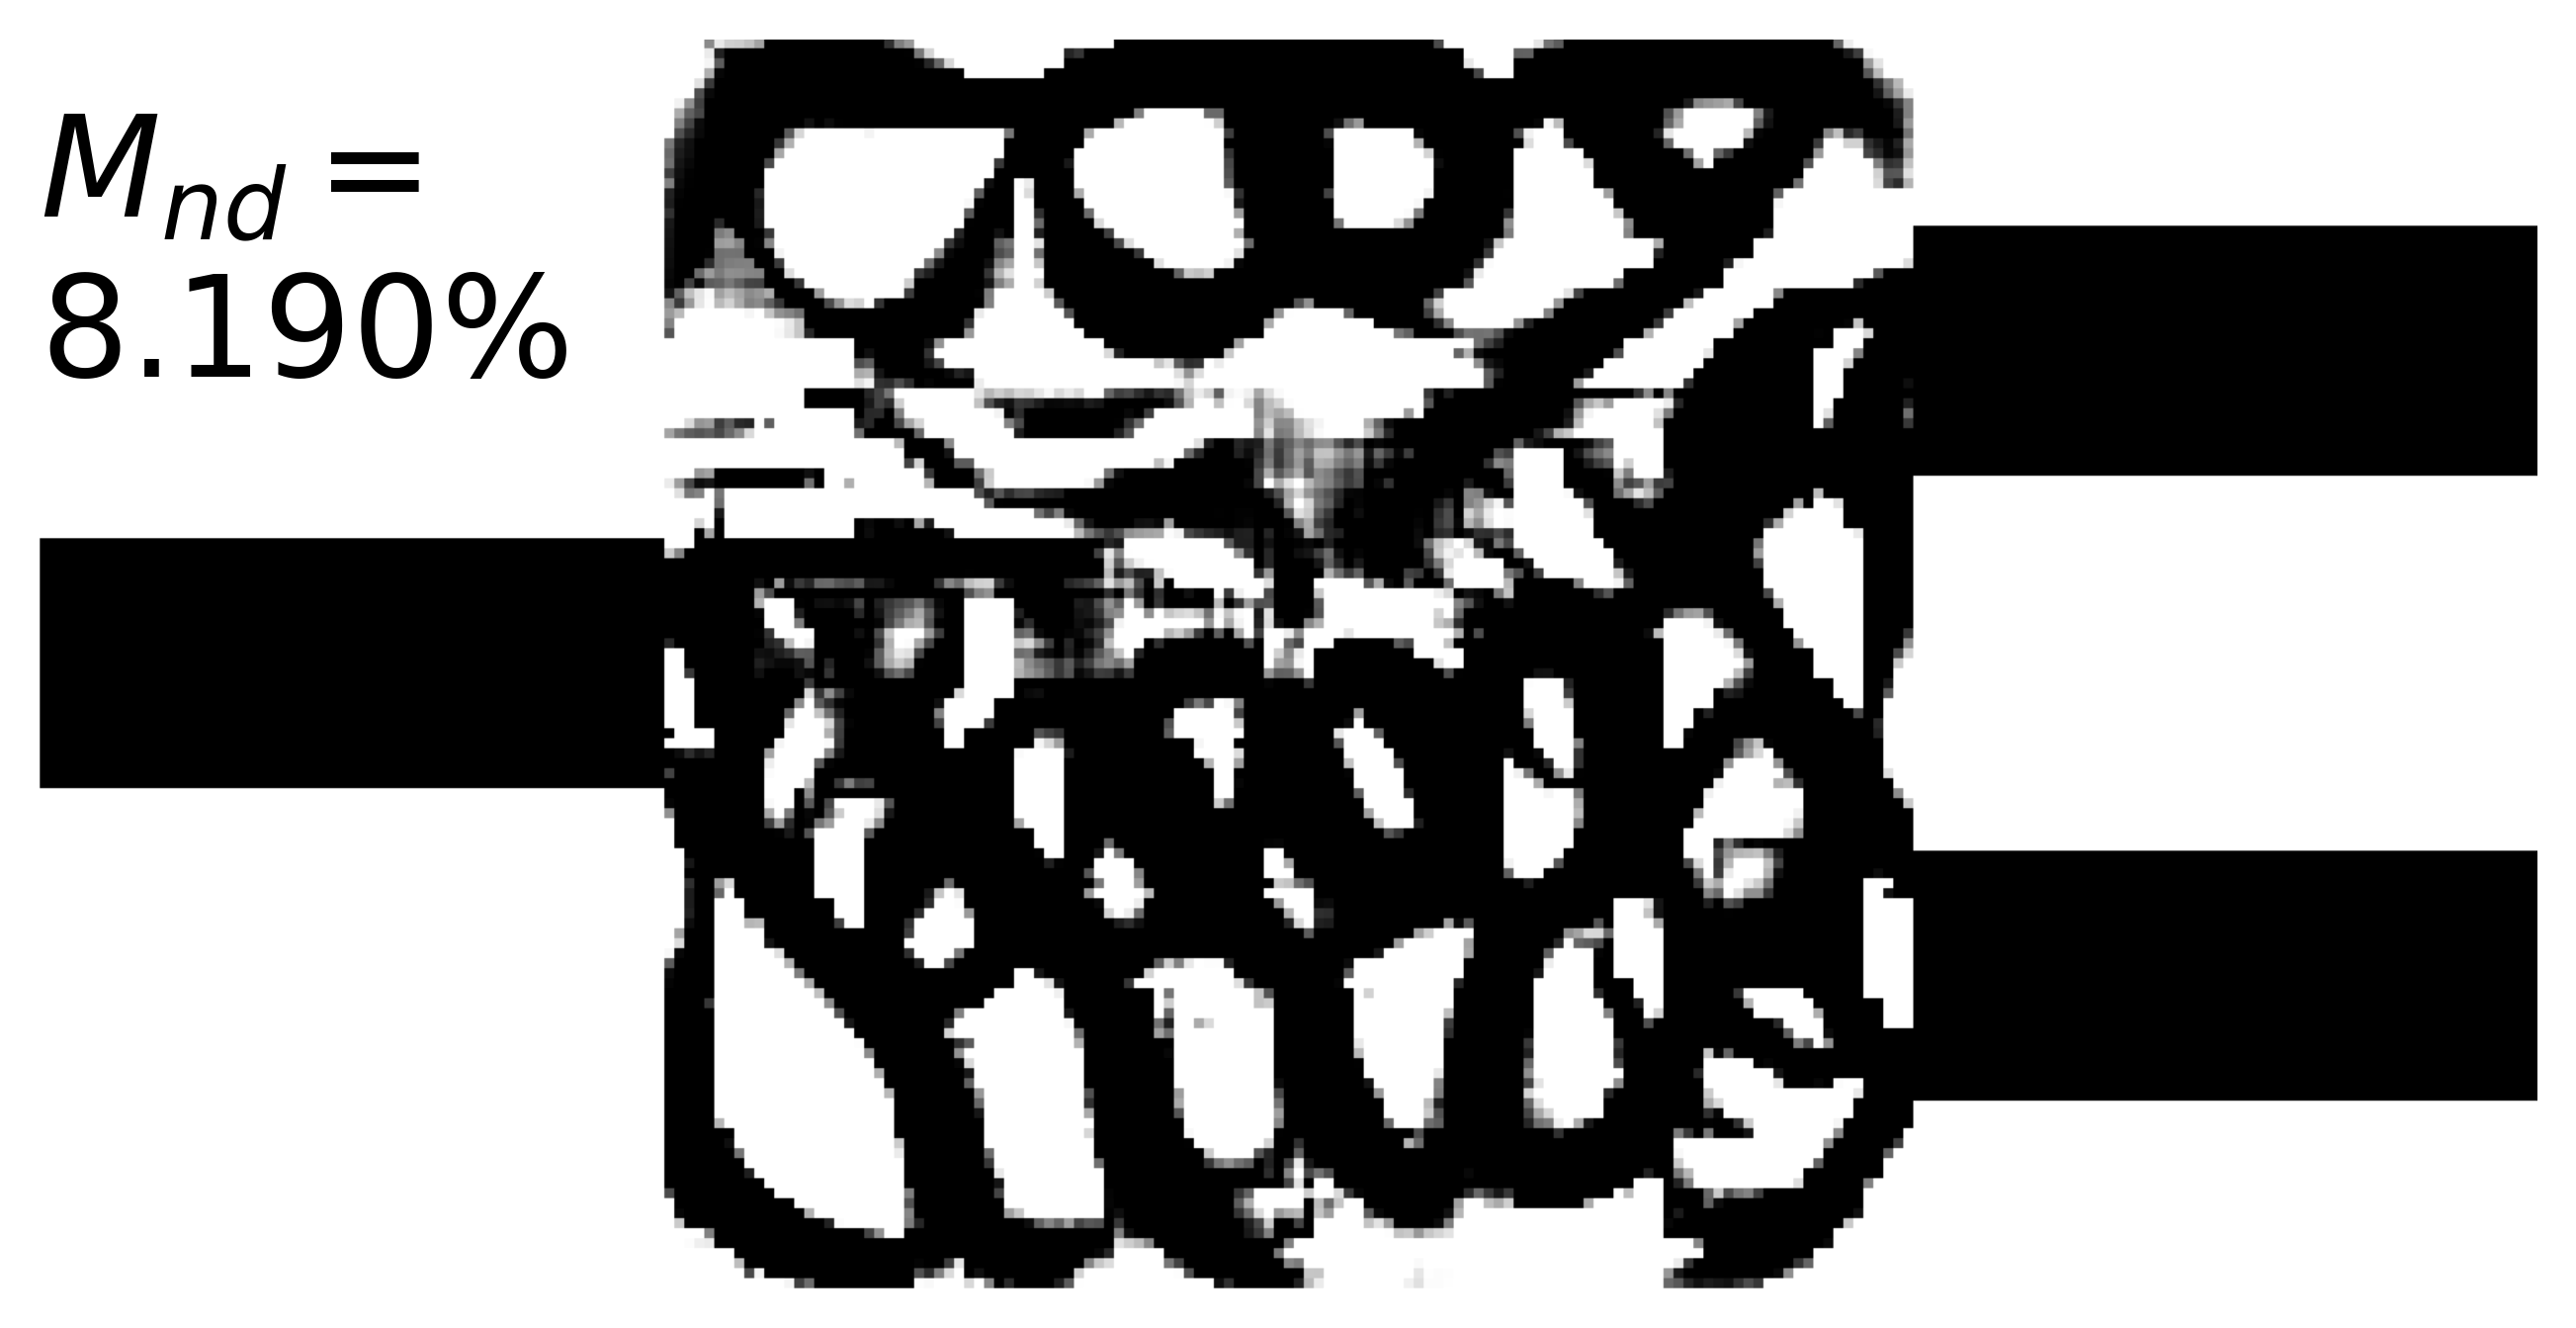
\includegraphics[width=0.24\textwidth]{image/results/wdm/L-BFGS-B/visualize_eps_cont_128.png} &
      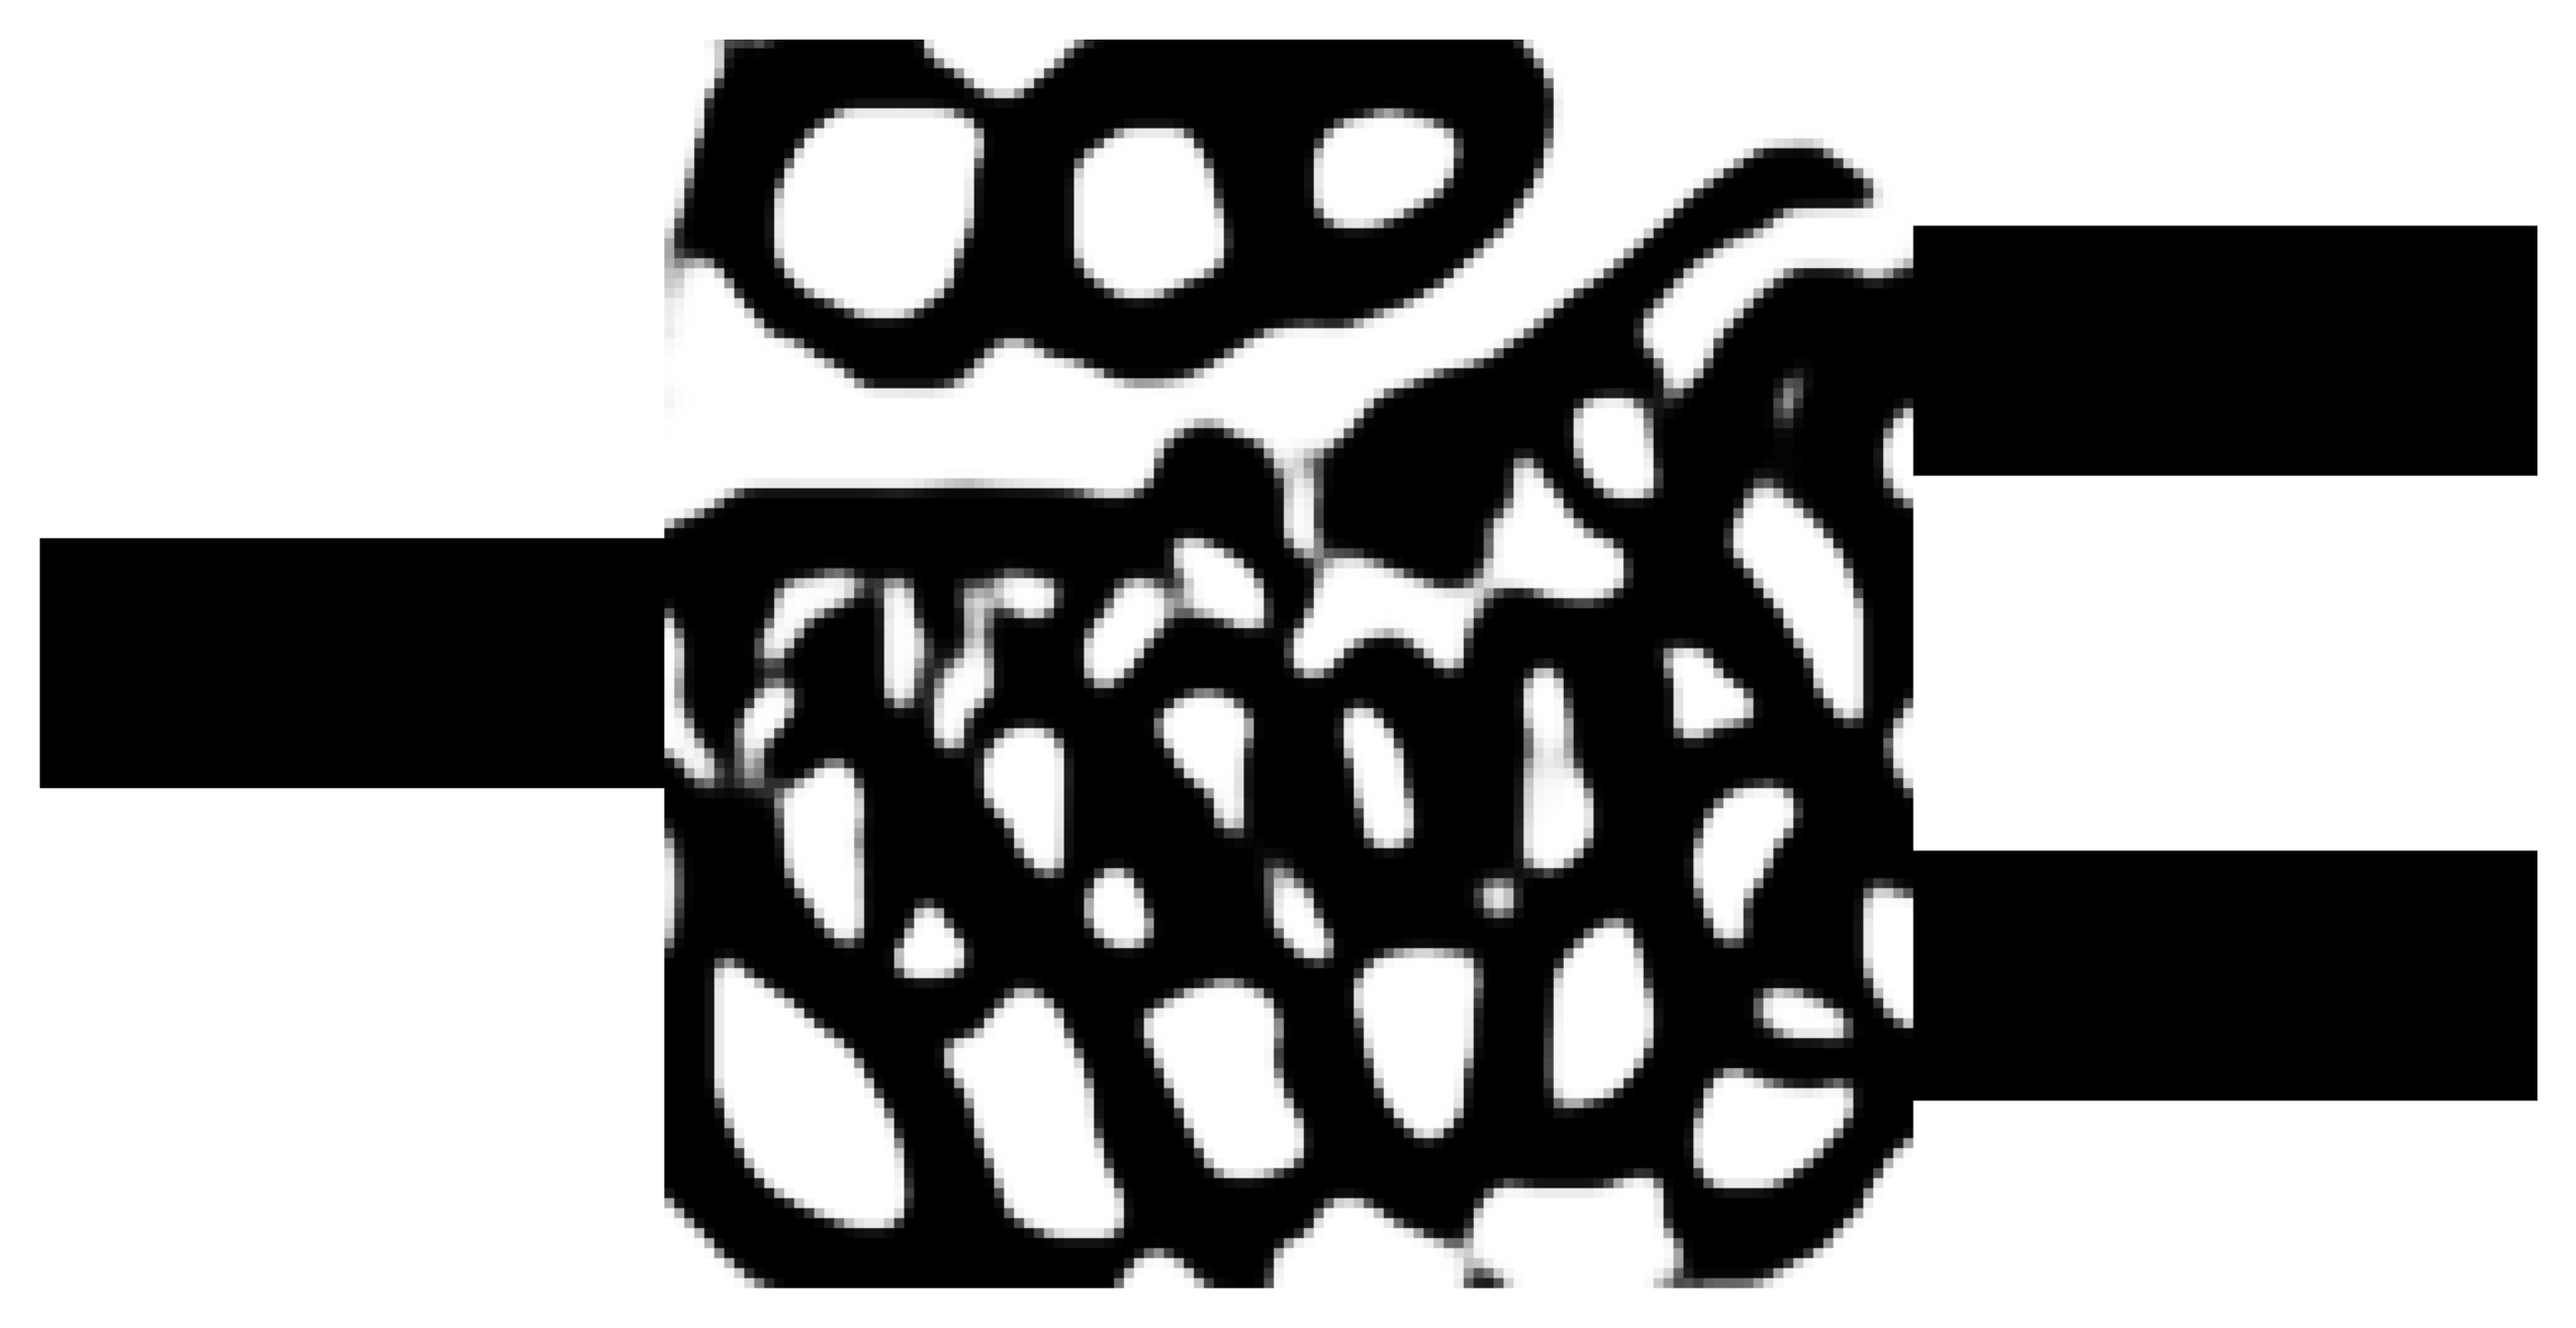
\includegraphics[width=0.24\textwidth]{image/results/wdm/L-BFGS-B/visualize_eps_disc_128.png} &
      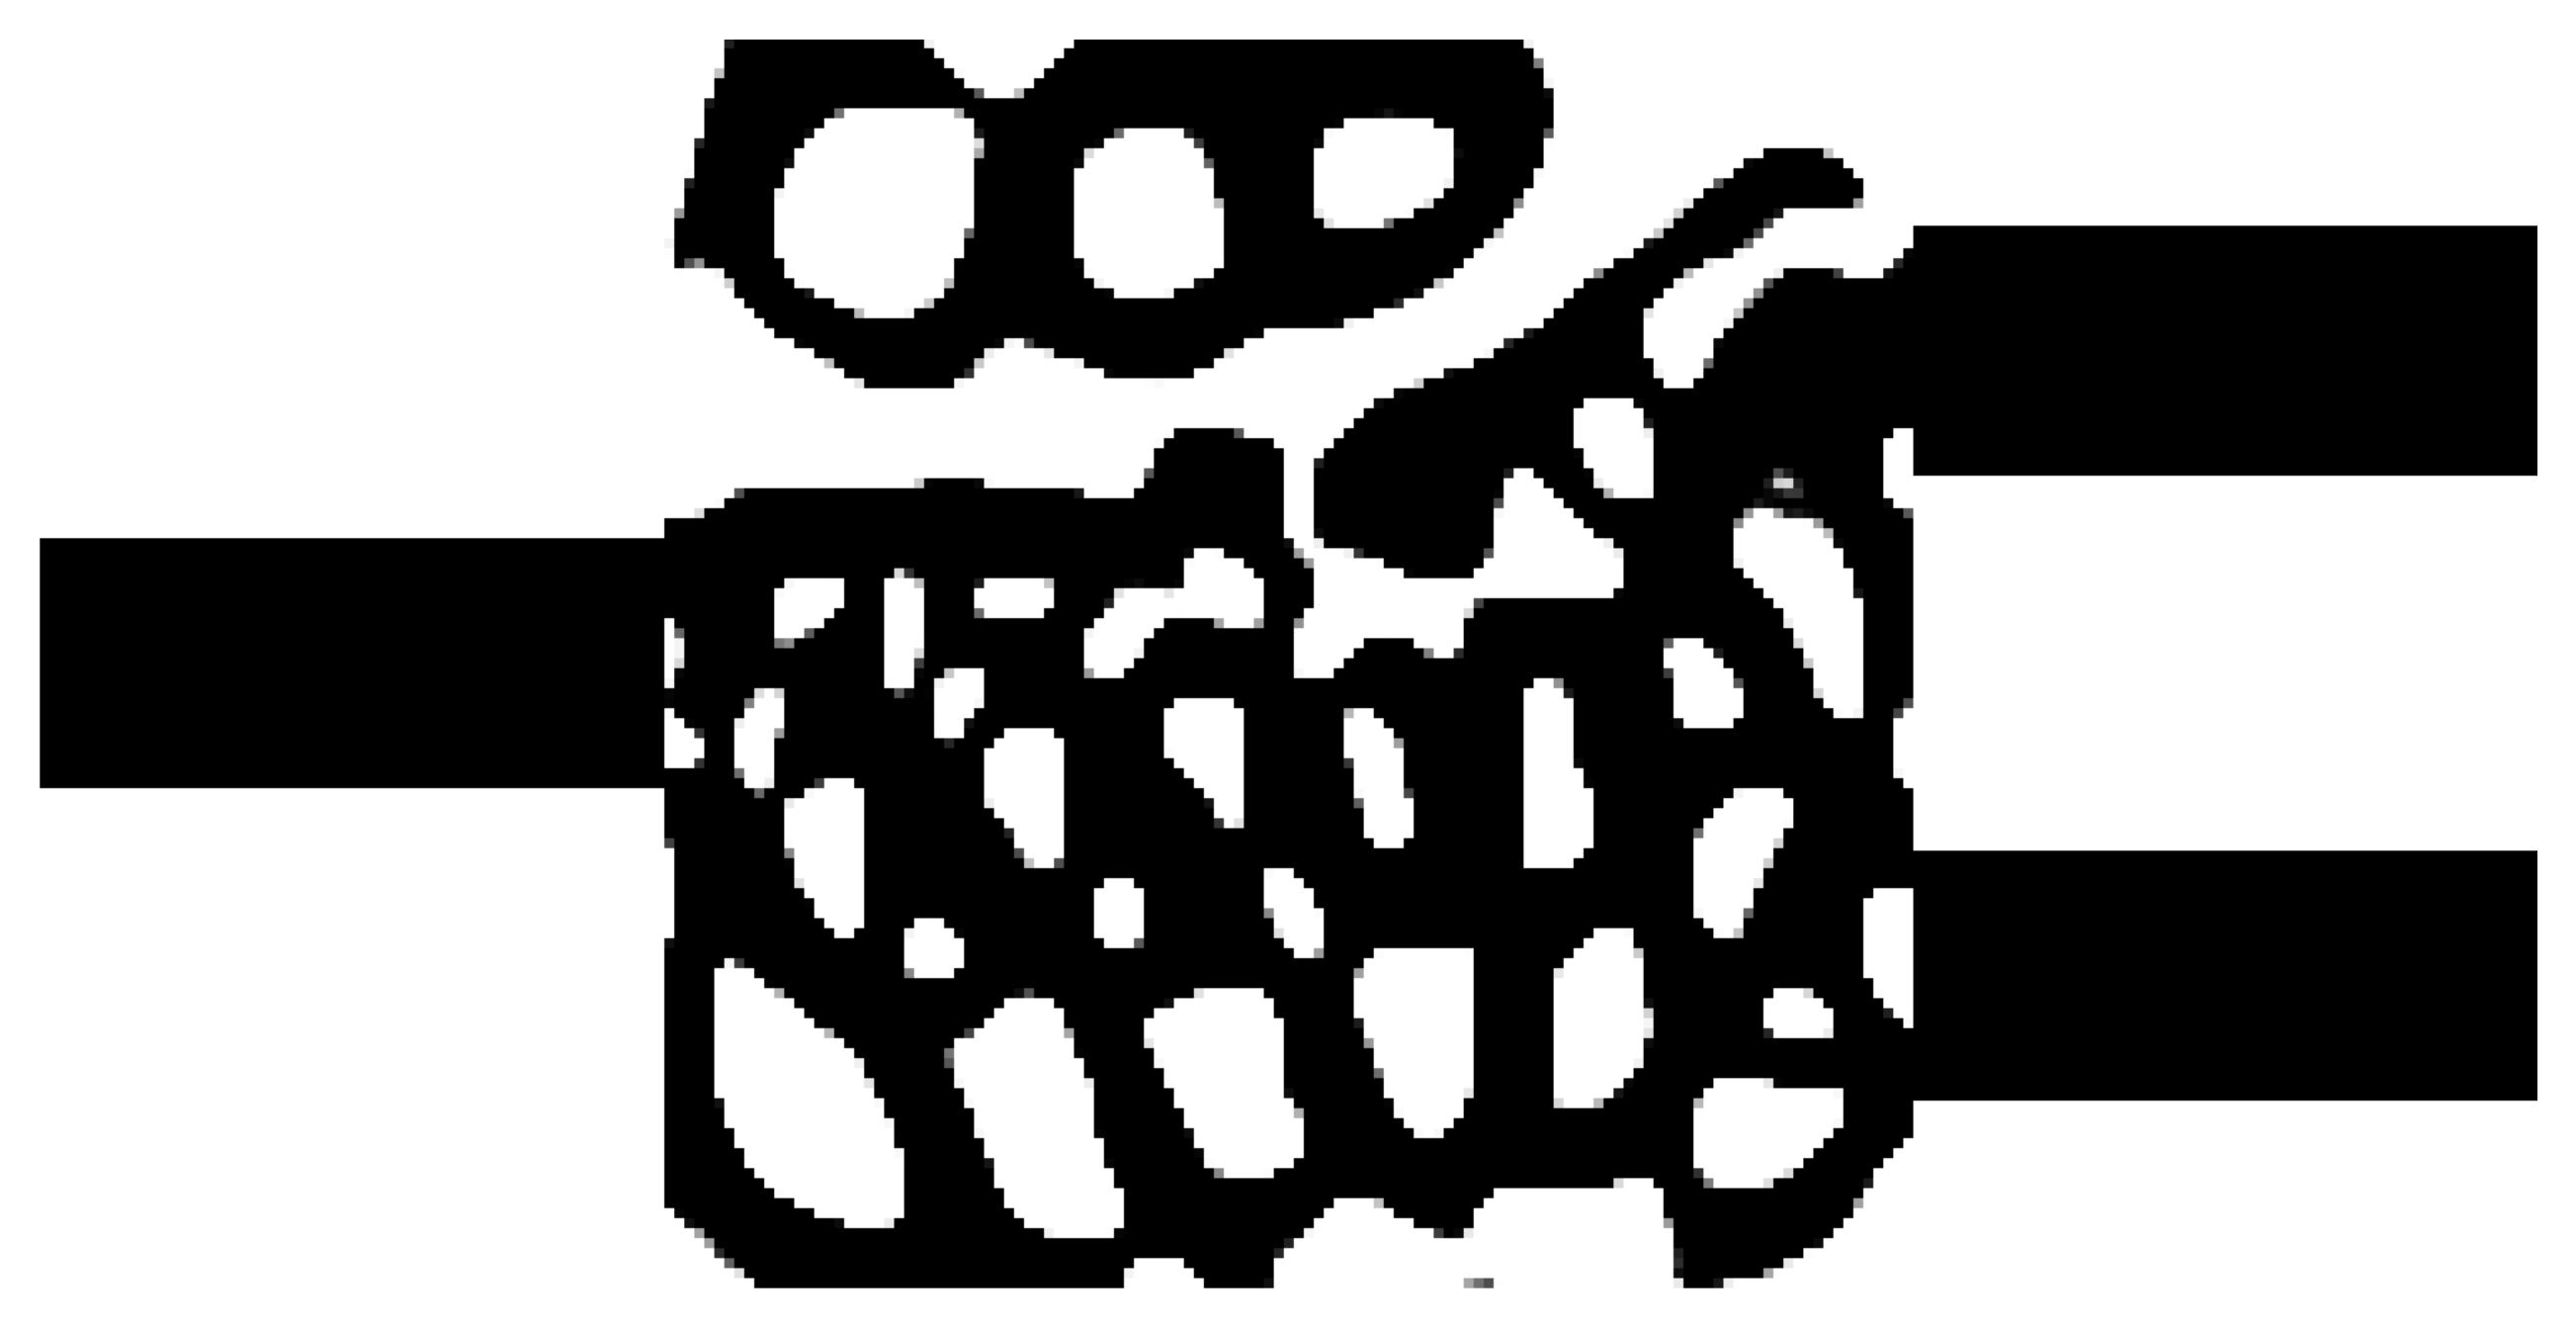
\includegraphics[width=0.24\textwidth]{image/results/wdm/L-BFGS-B/visualize_eps_fab_128.png} \\
      \cline{2-4}
      &
      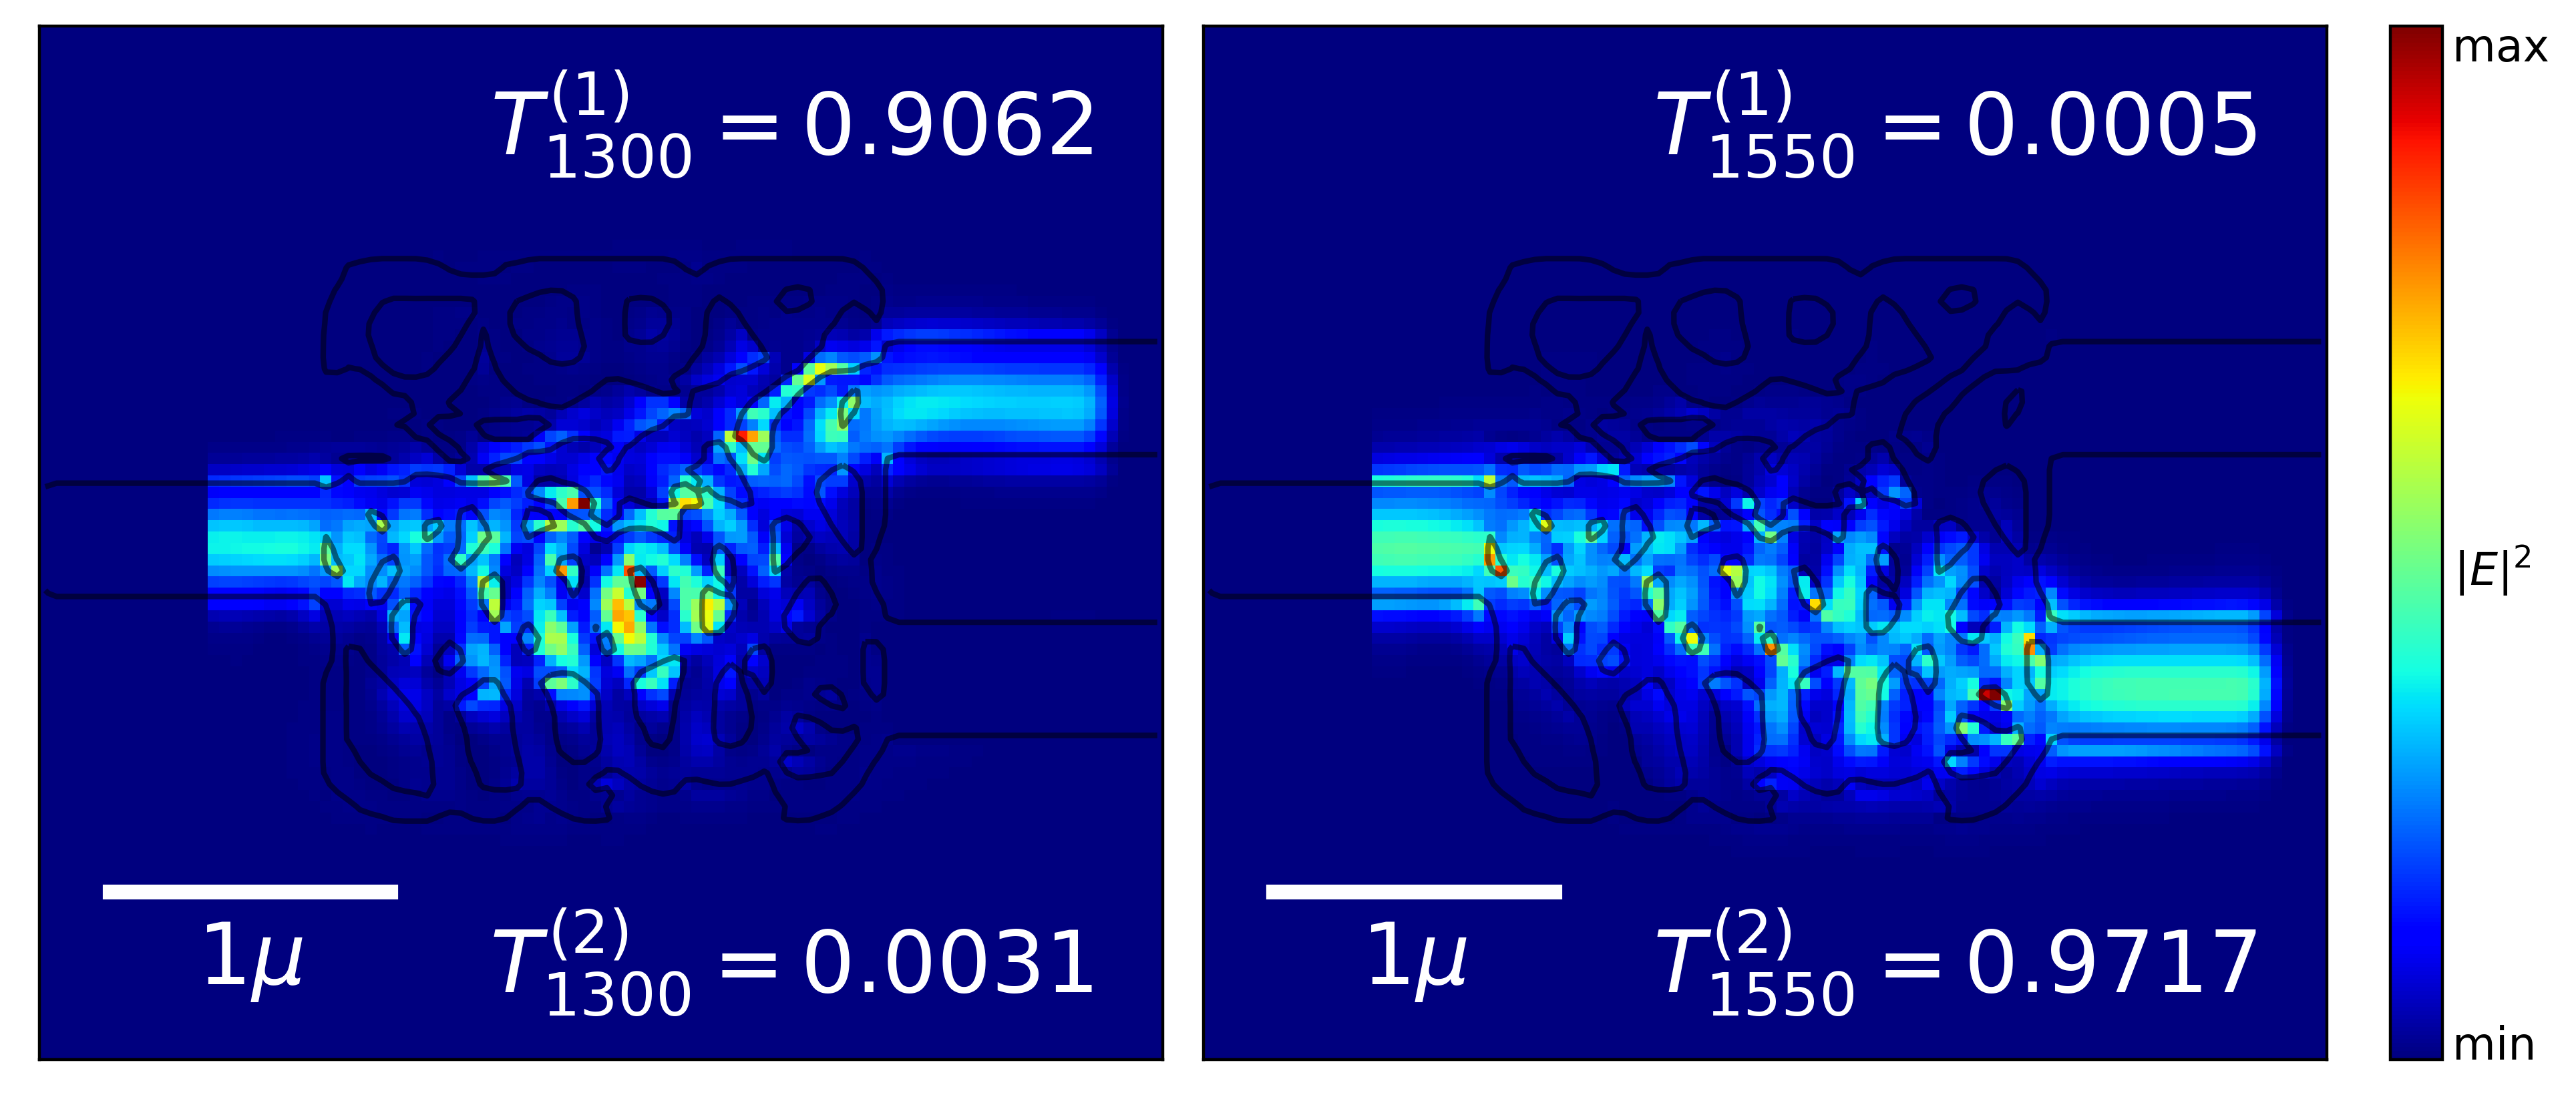
\includegraphics[width=0.50\textwidth]{image/results/wdm/L-BFGS-B/visualize_field_cont_128.png} &
      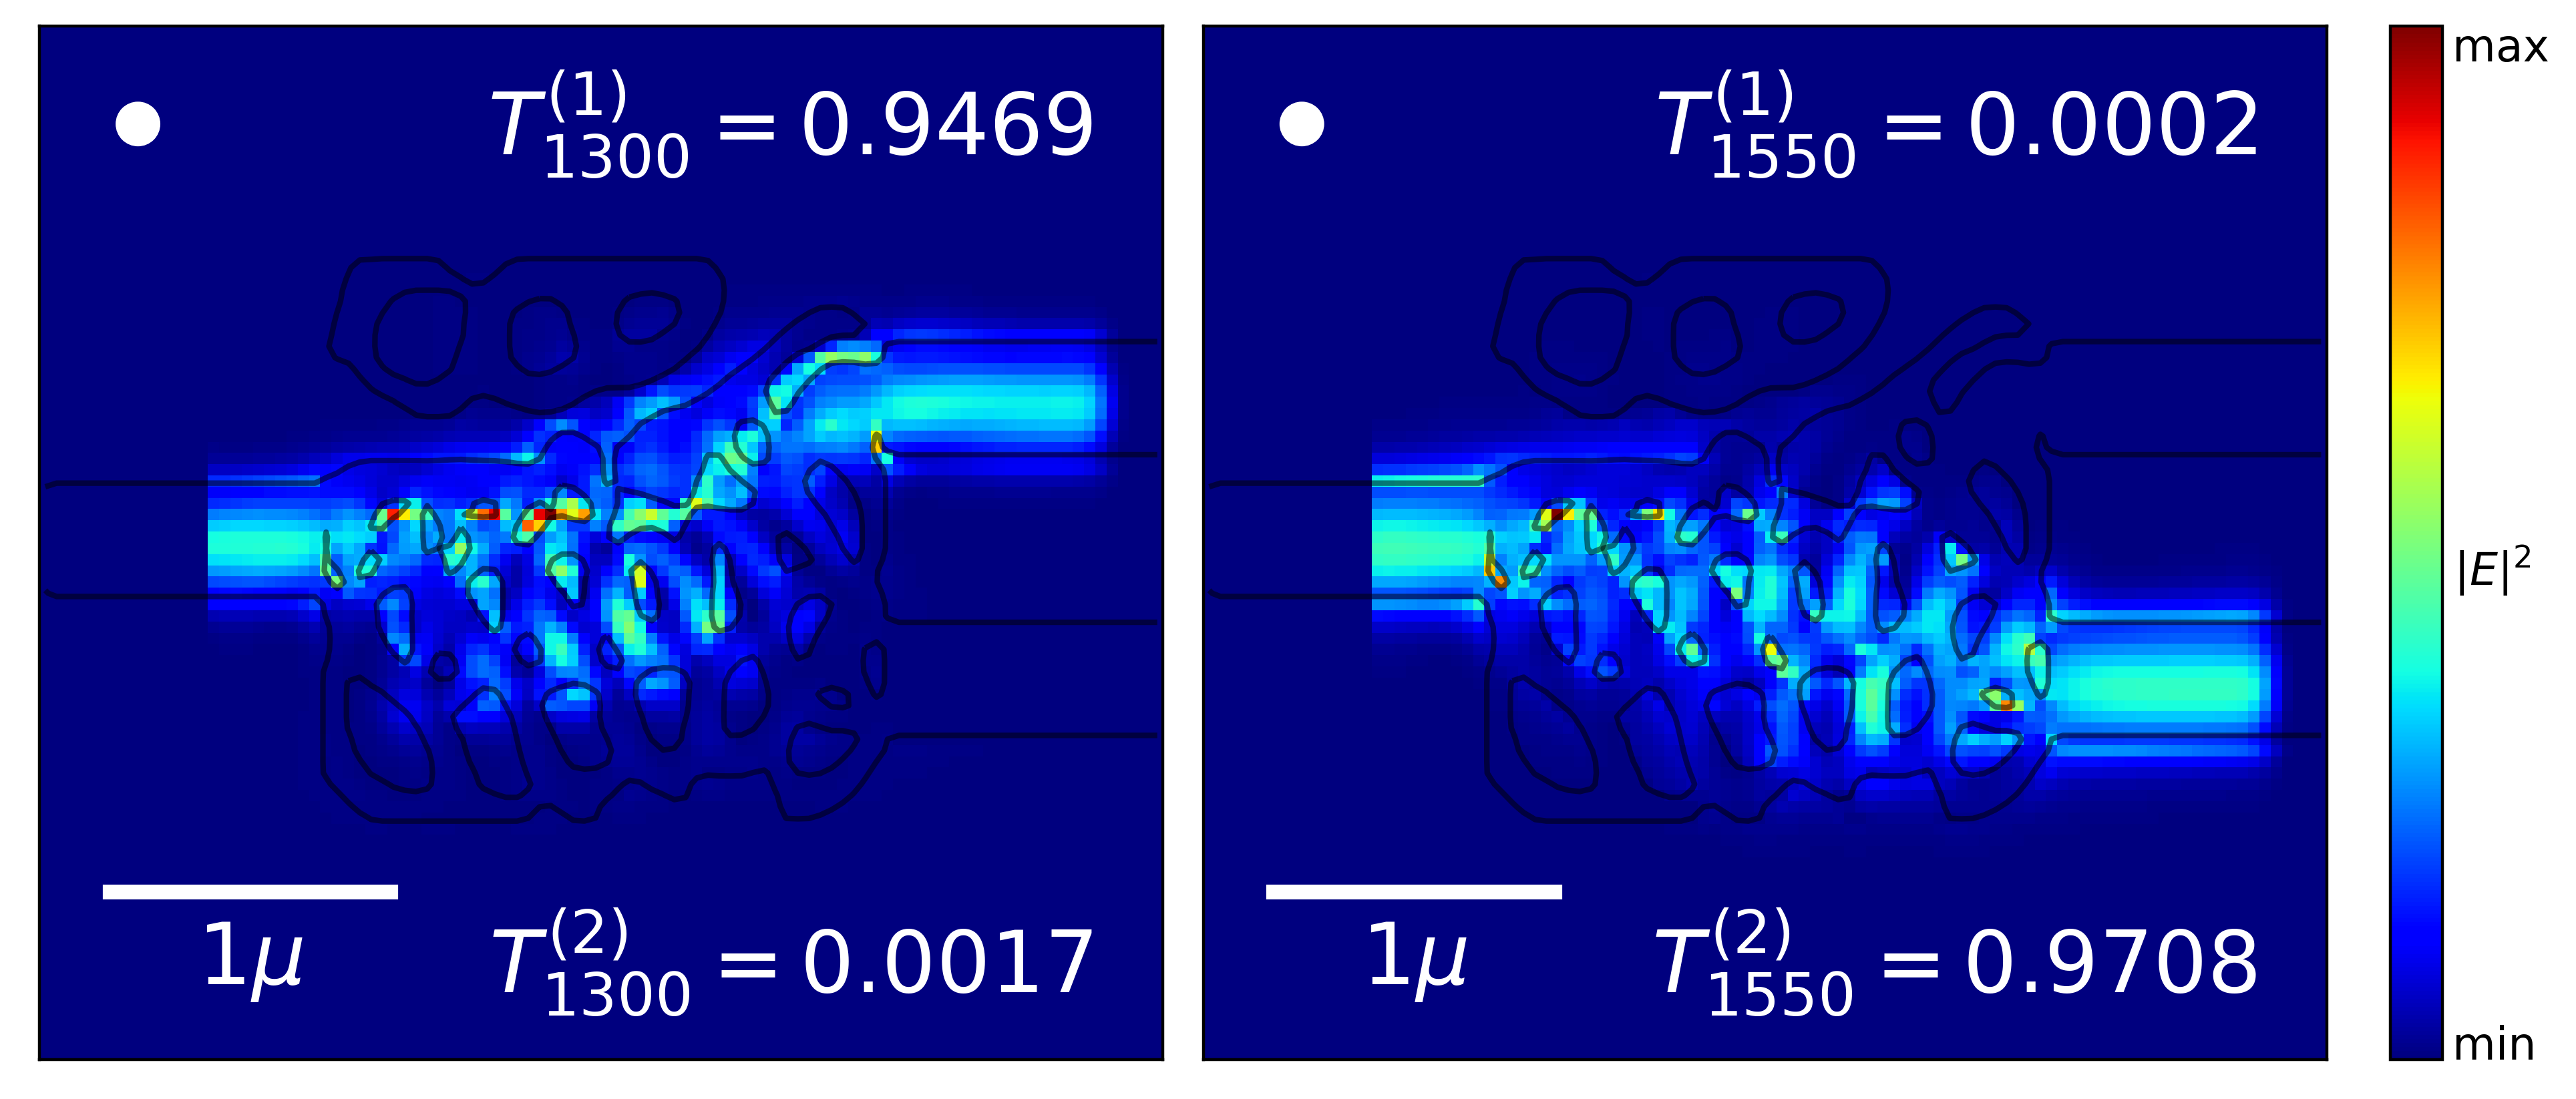
\includegraphics[width=0.50\textwidth]{image/results/wdm/L-BFGS-B/visualize_field_disc_128.png} &
      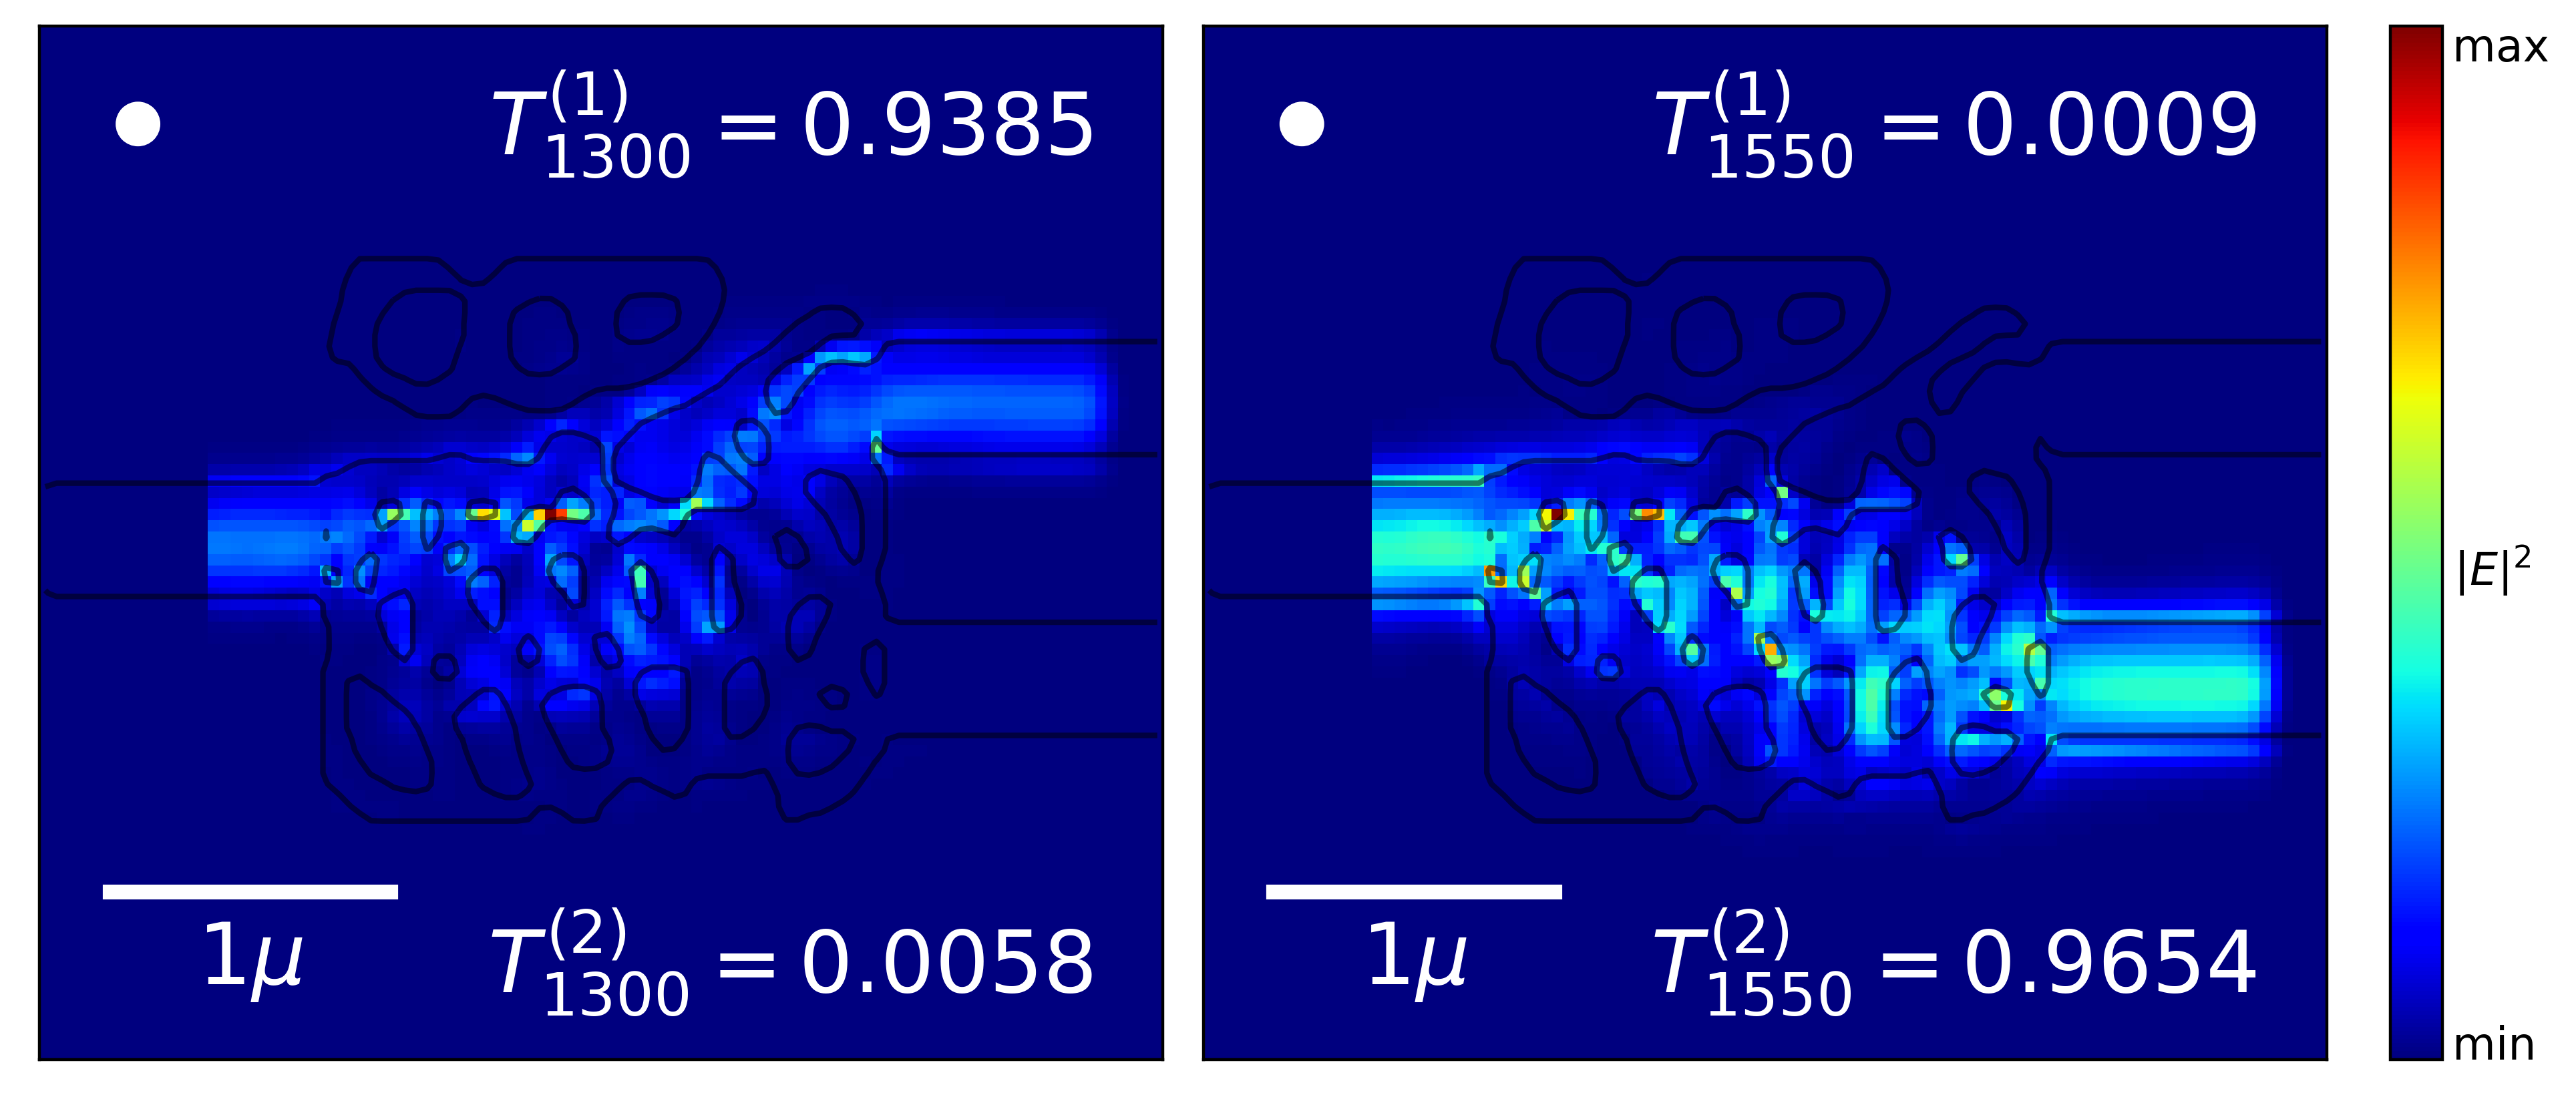
\includegraphics[width=0.50\textwidth]{image/results/wdm/L-BFGS-B/visualize_field_fab_128.png} \\
    \hline
      \multirow{2}{*}{256} &
      
\includegraphics[width=0.24\textwidth]{image/results/wdm/L-BFGS-B/visualize_eps_cont_256.png} &
      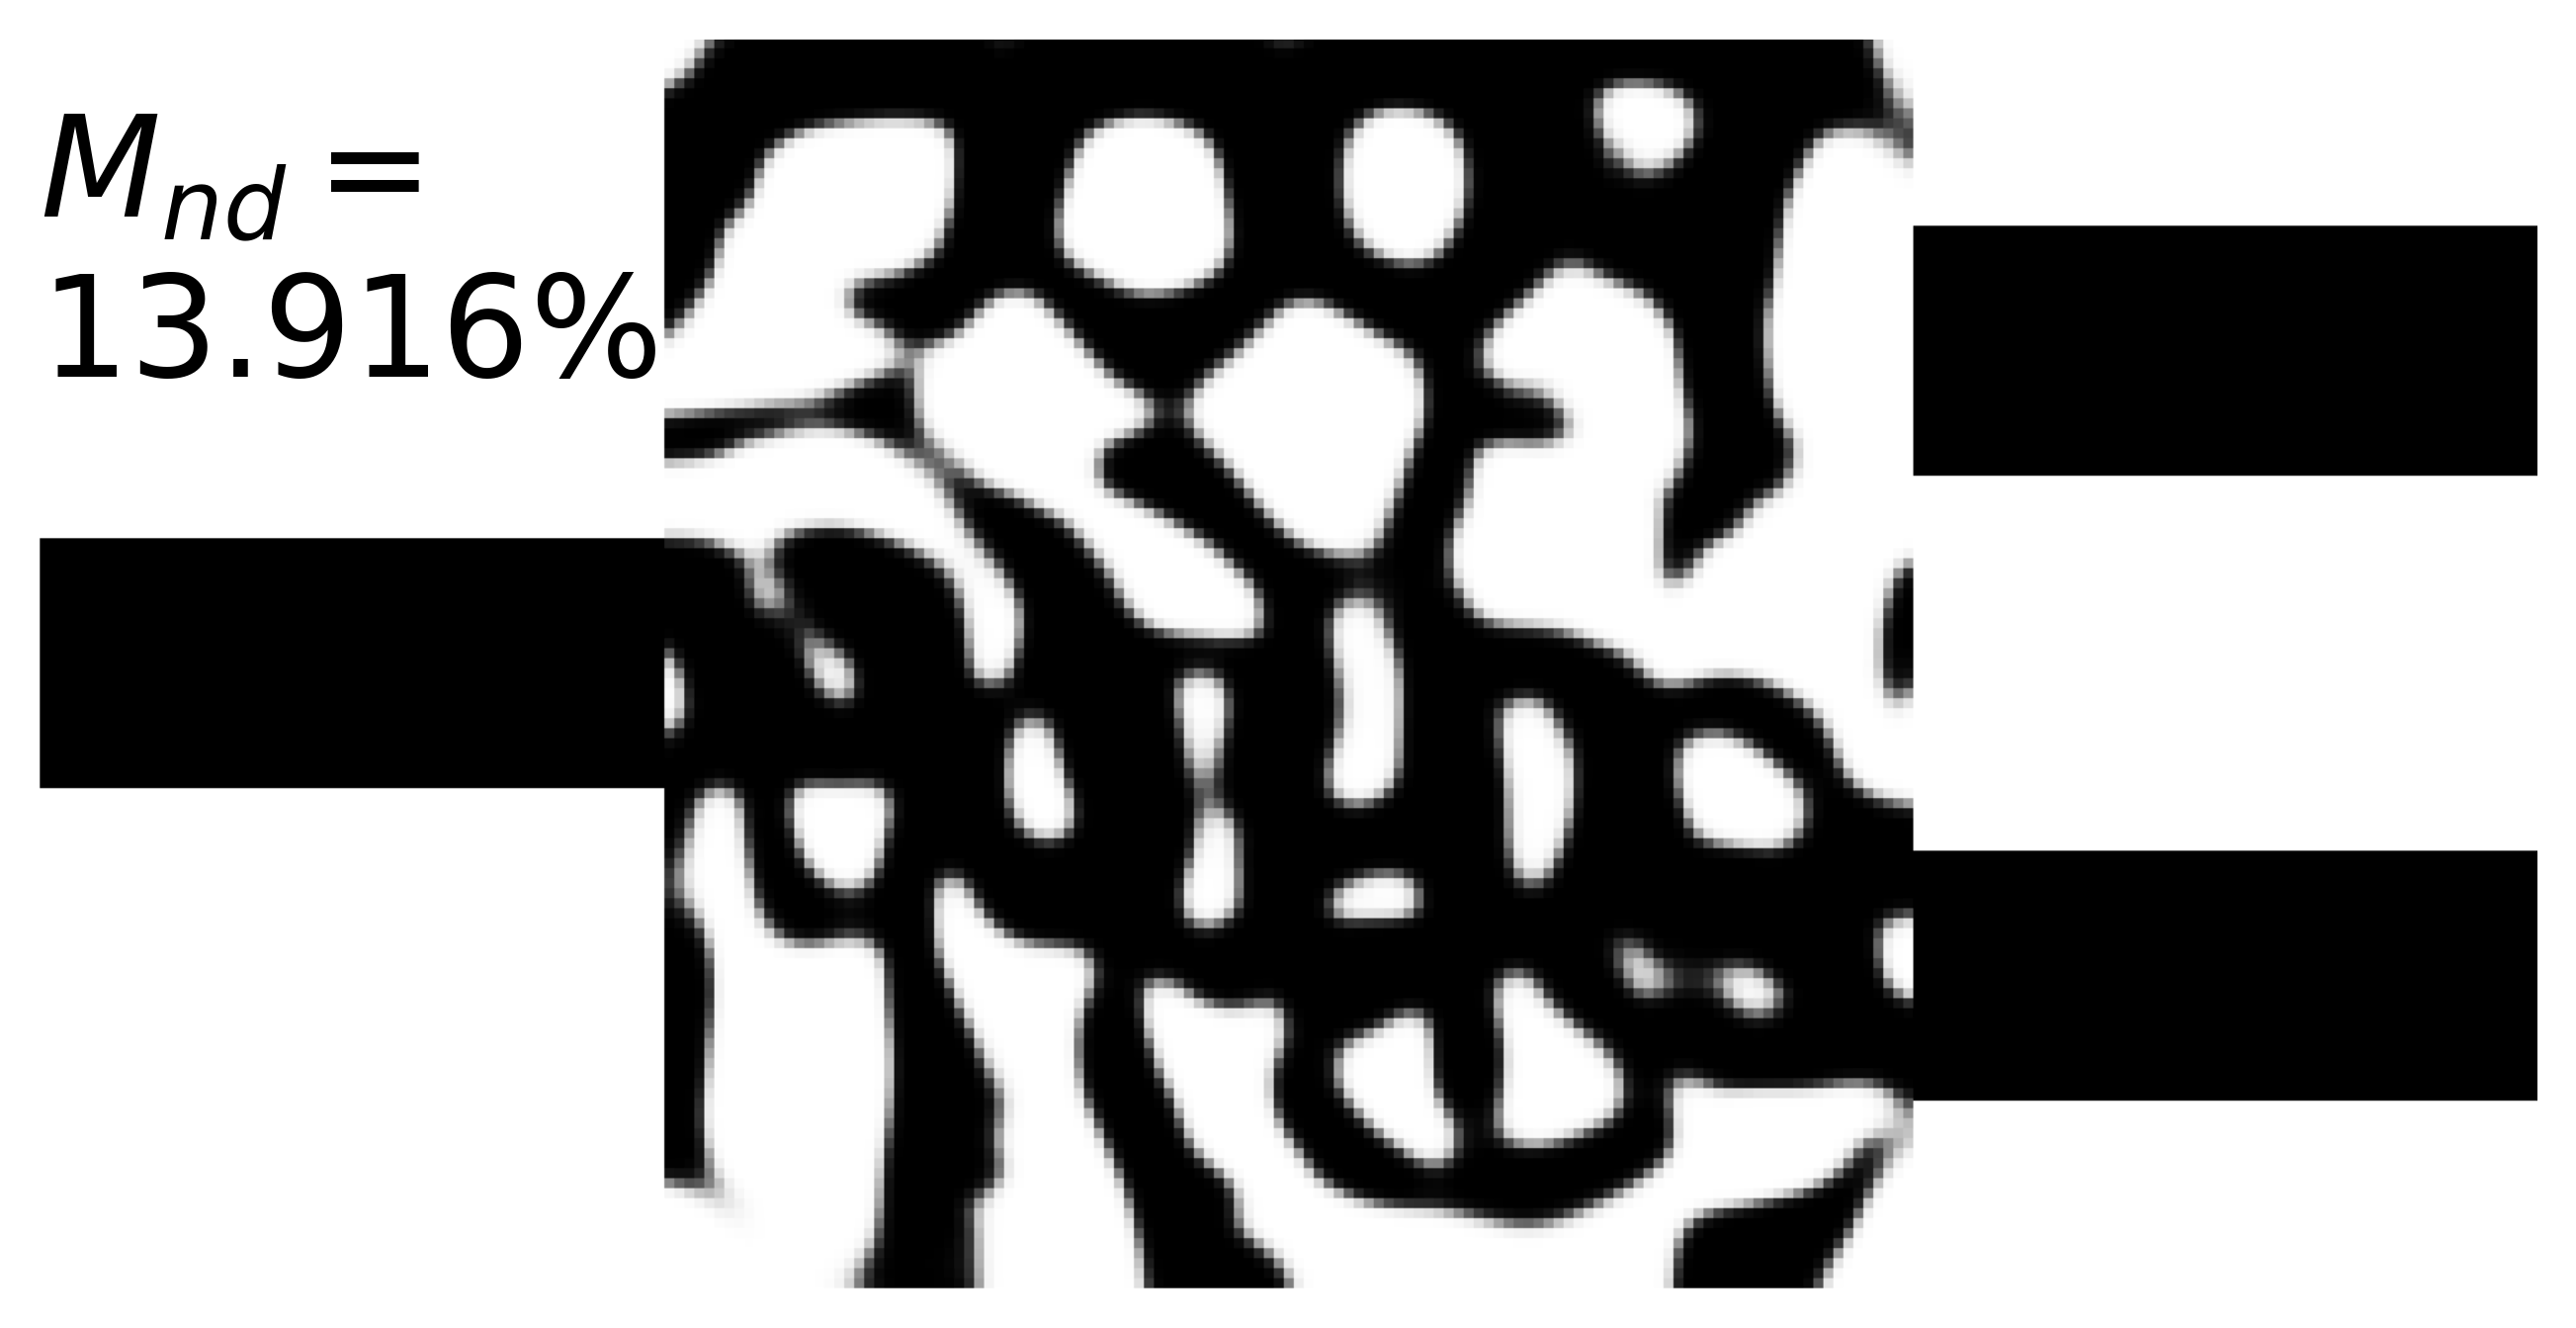
\includegraphics[width=0.24\textwidth]{image/results/wdm/L-BFGS-B/visualize_eps_disc_256.png} &
      
\includegraphics[width=0.24\textwidth]{image/results/wdm/L-BFGS-B/visualize_eps_fab_256.png} \\
      \cline{2-4}
      &
      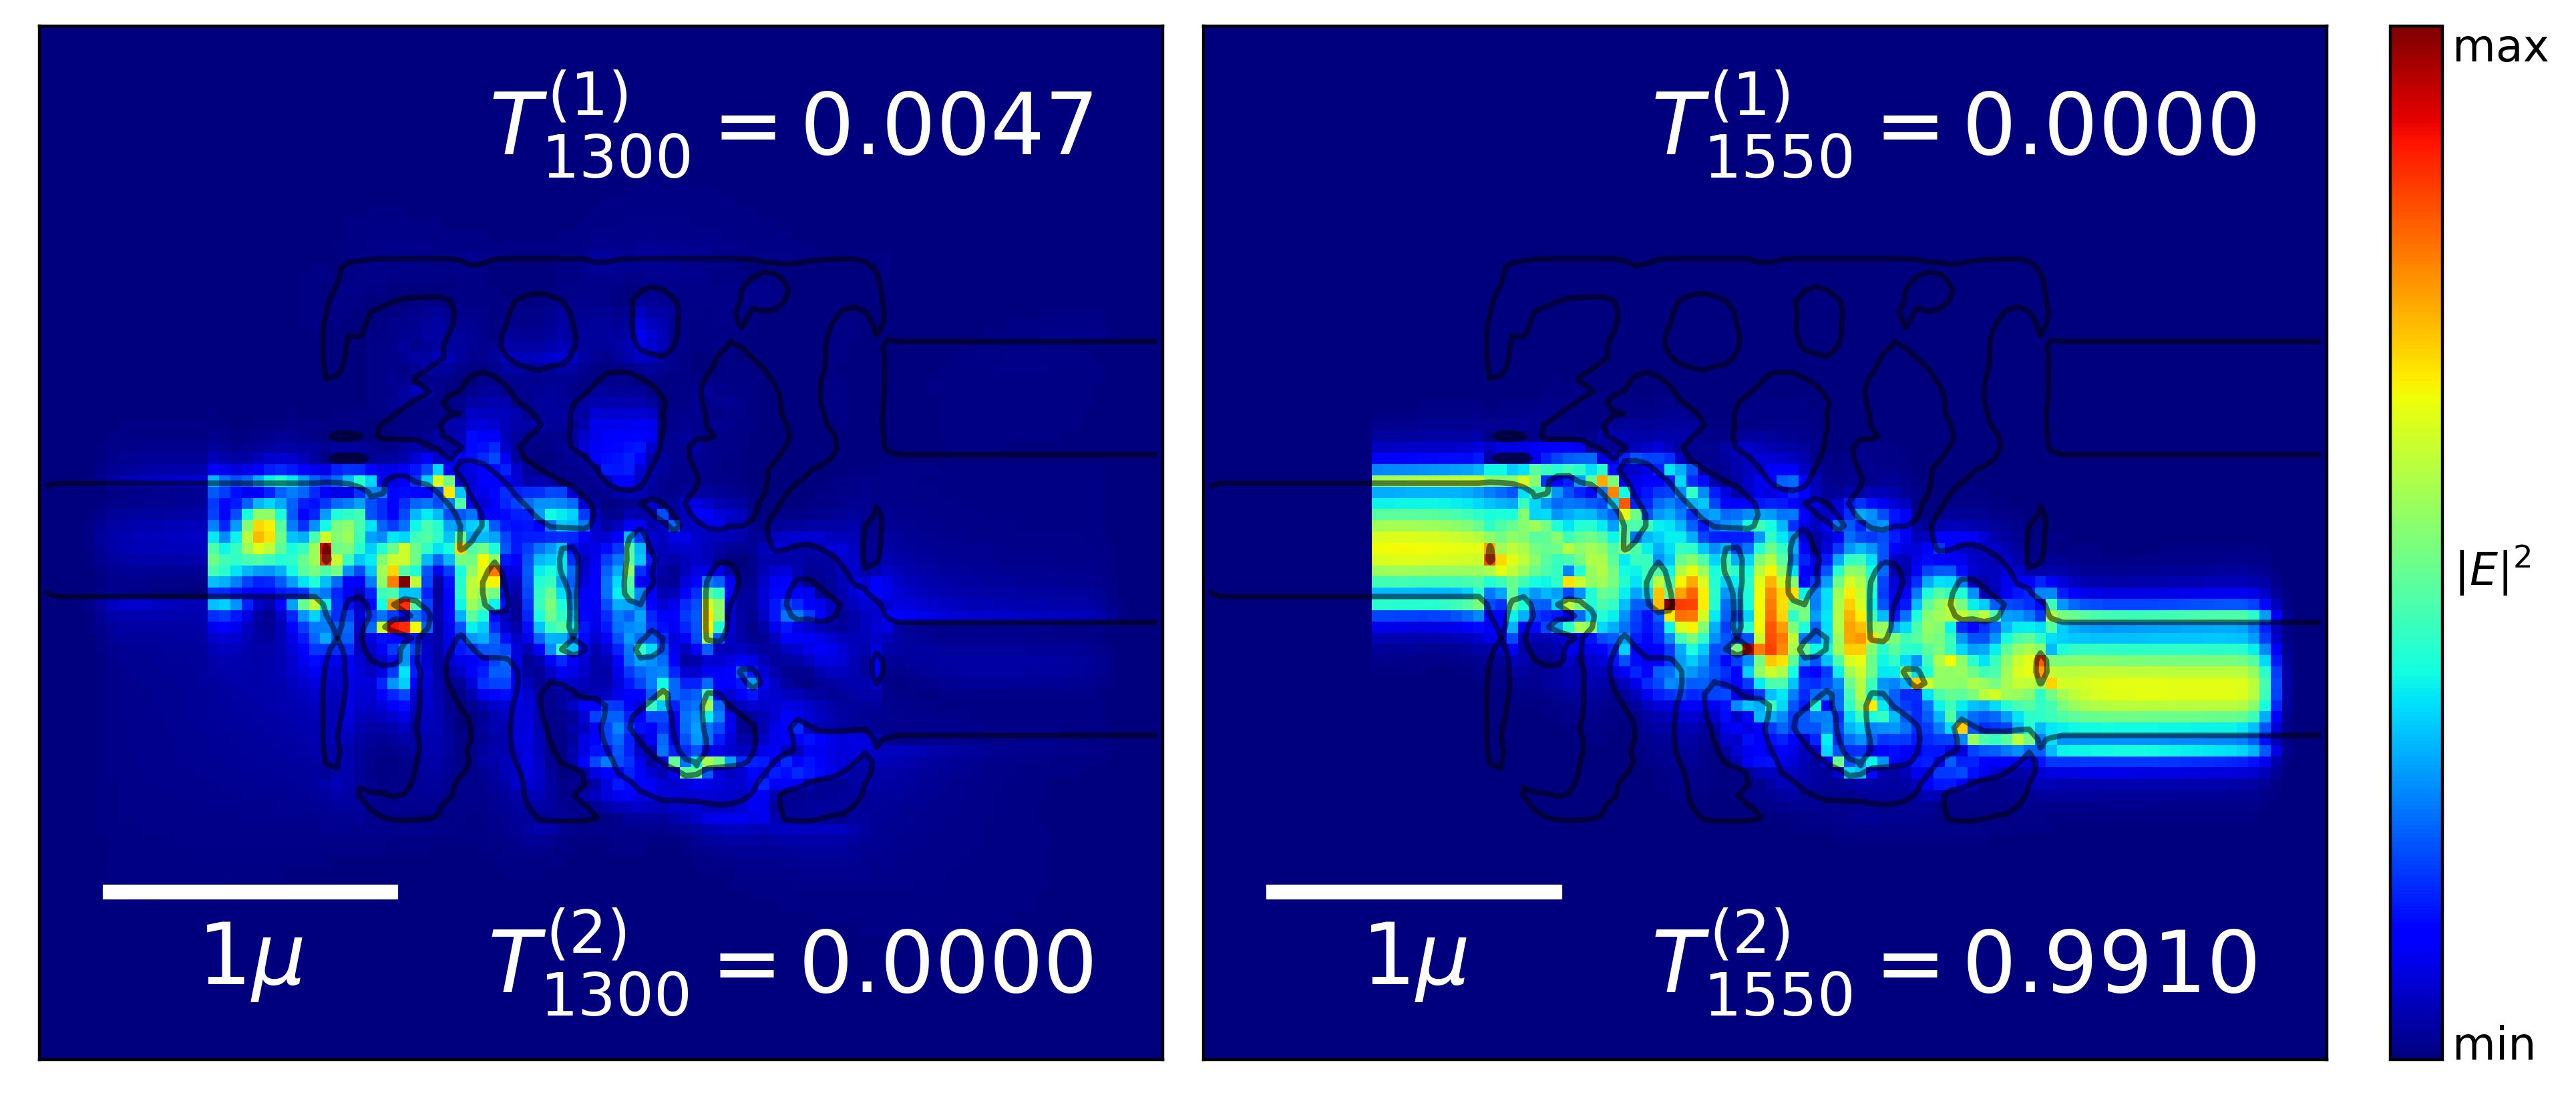
\includegraphics[width=0.50\textwidth]{image/results/wdm/L-BFGS-B/visualize_field_cont_256.png} &
      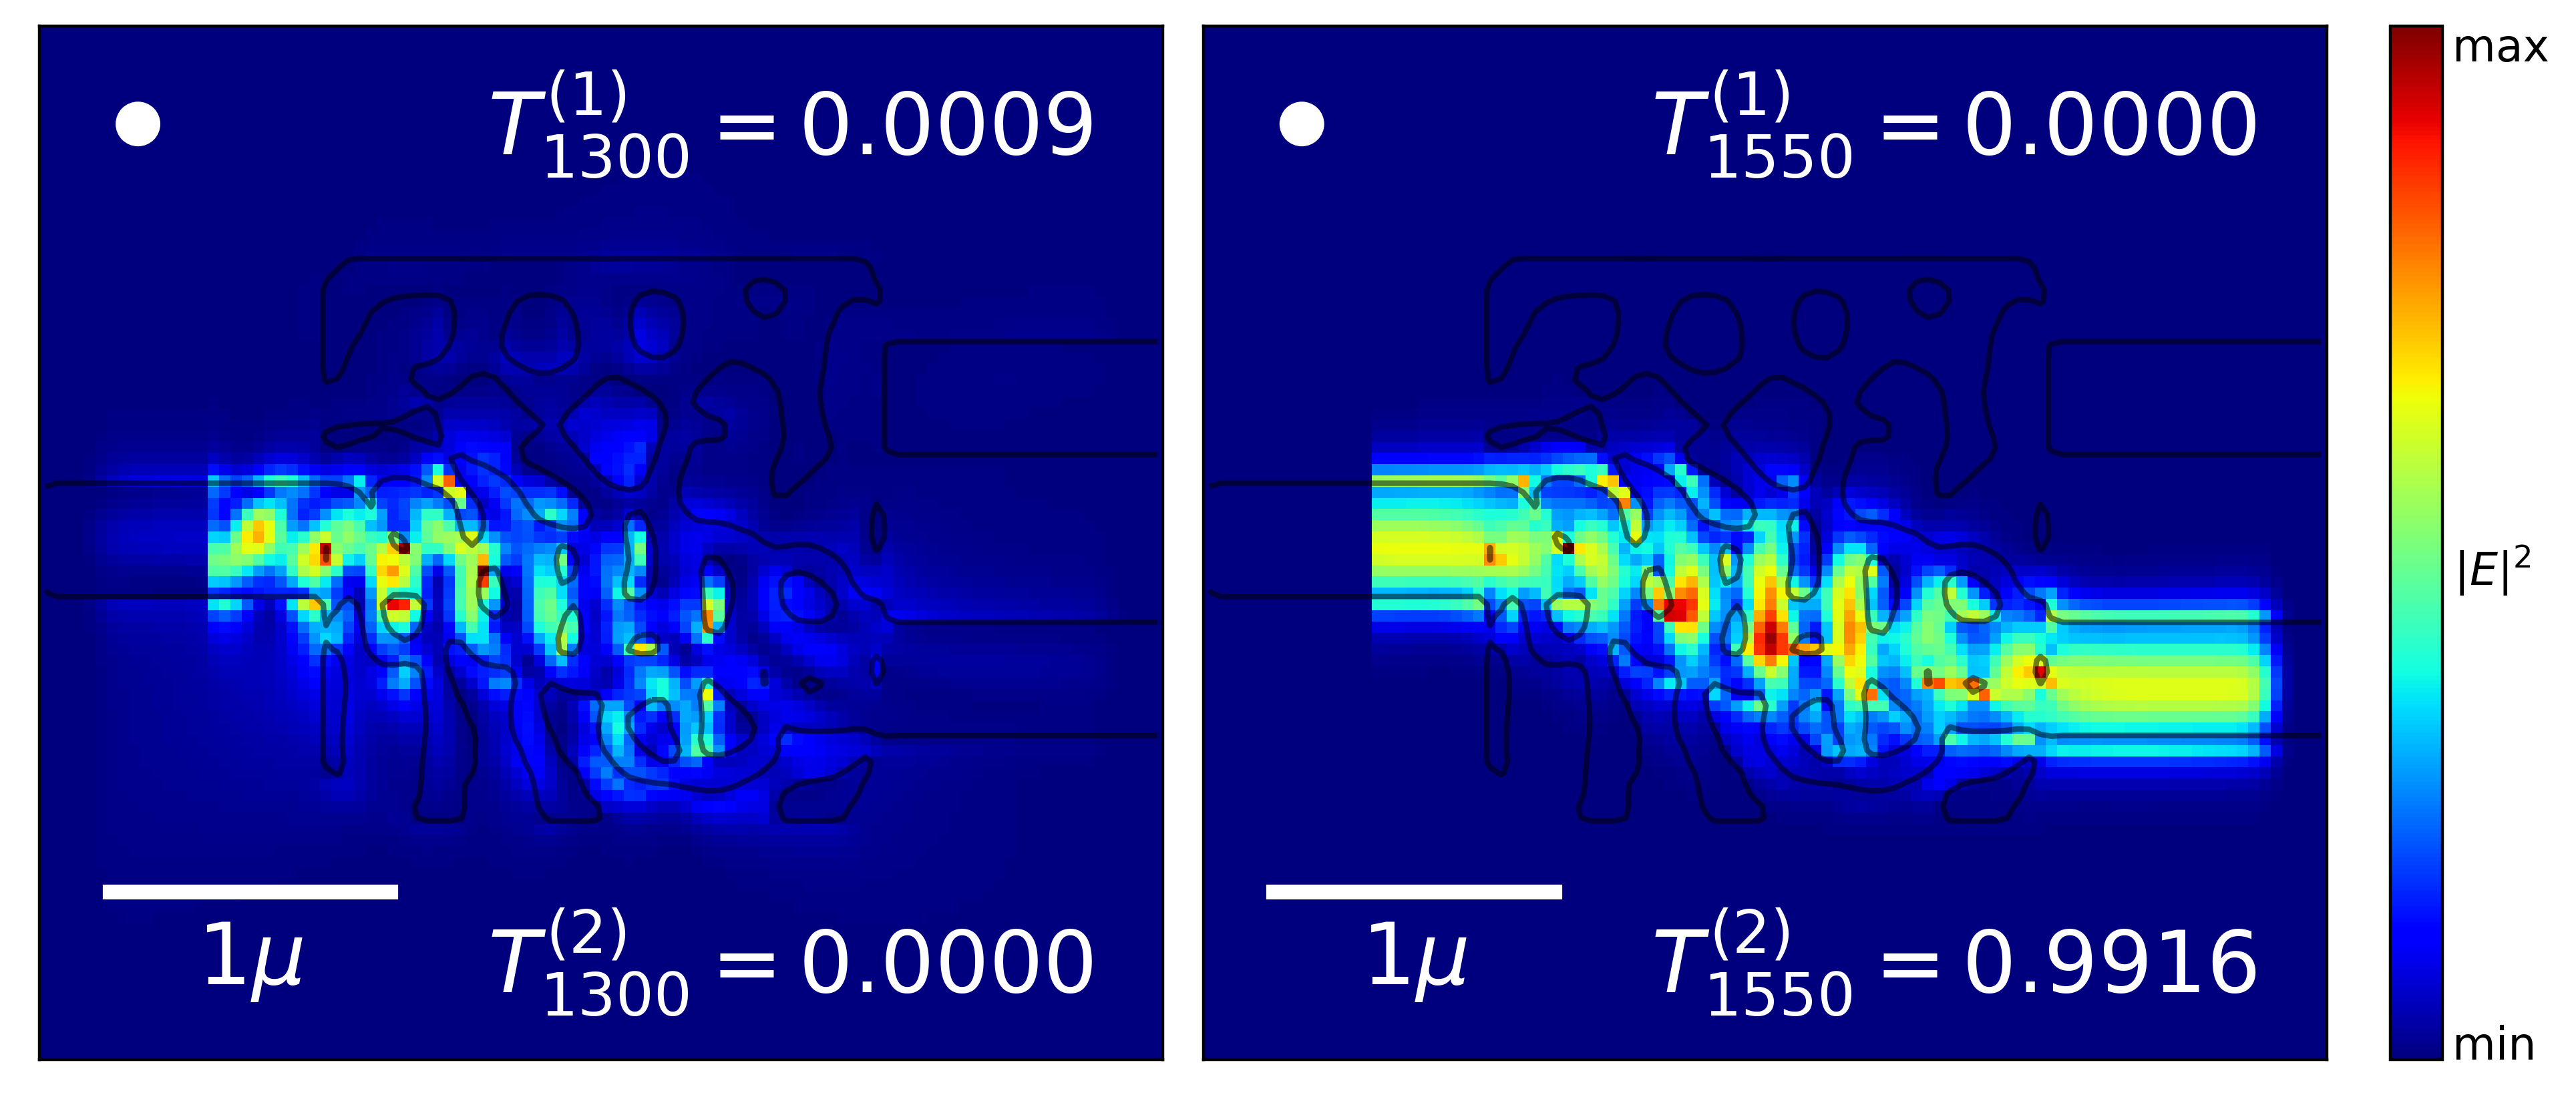
\includegraphics[width=0.50\textwidth]{image/results/wdm/L-BFGS-B/visualize_field_disc_256.png} &
      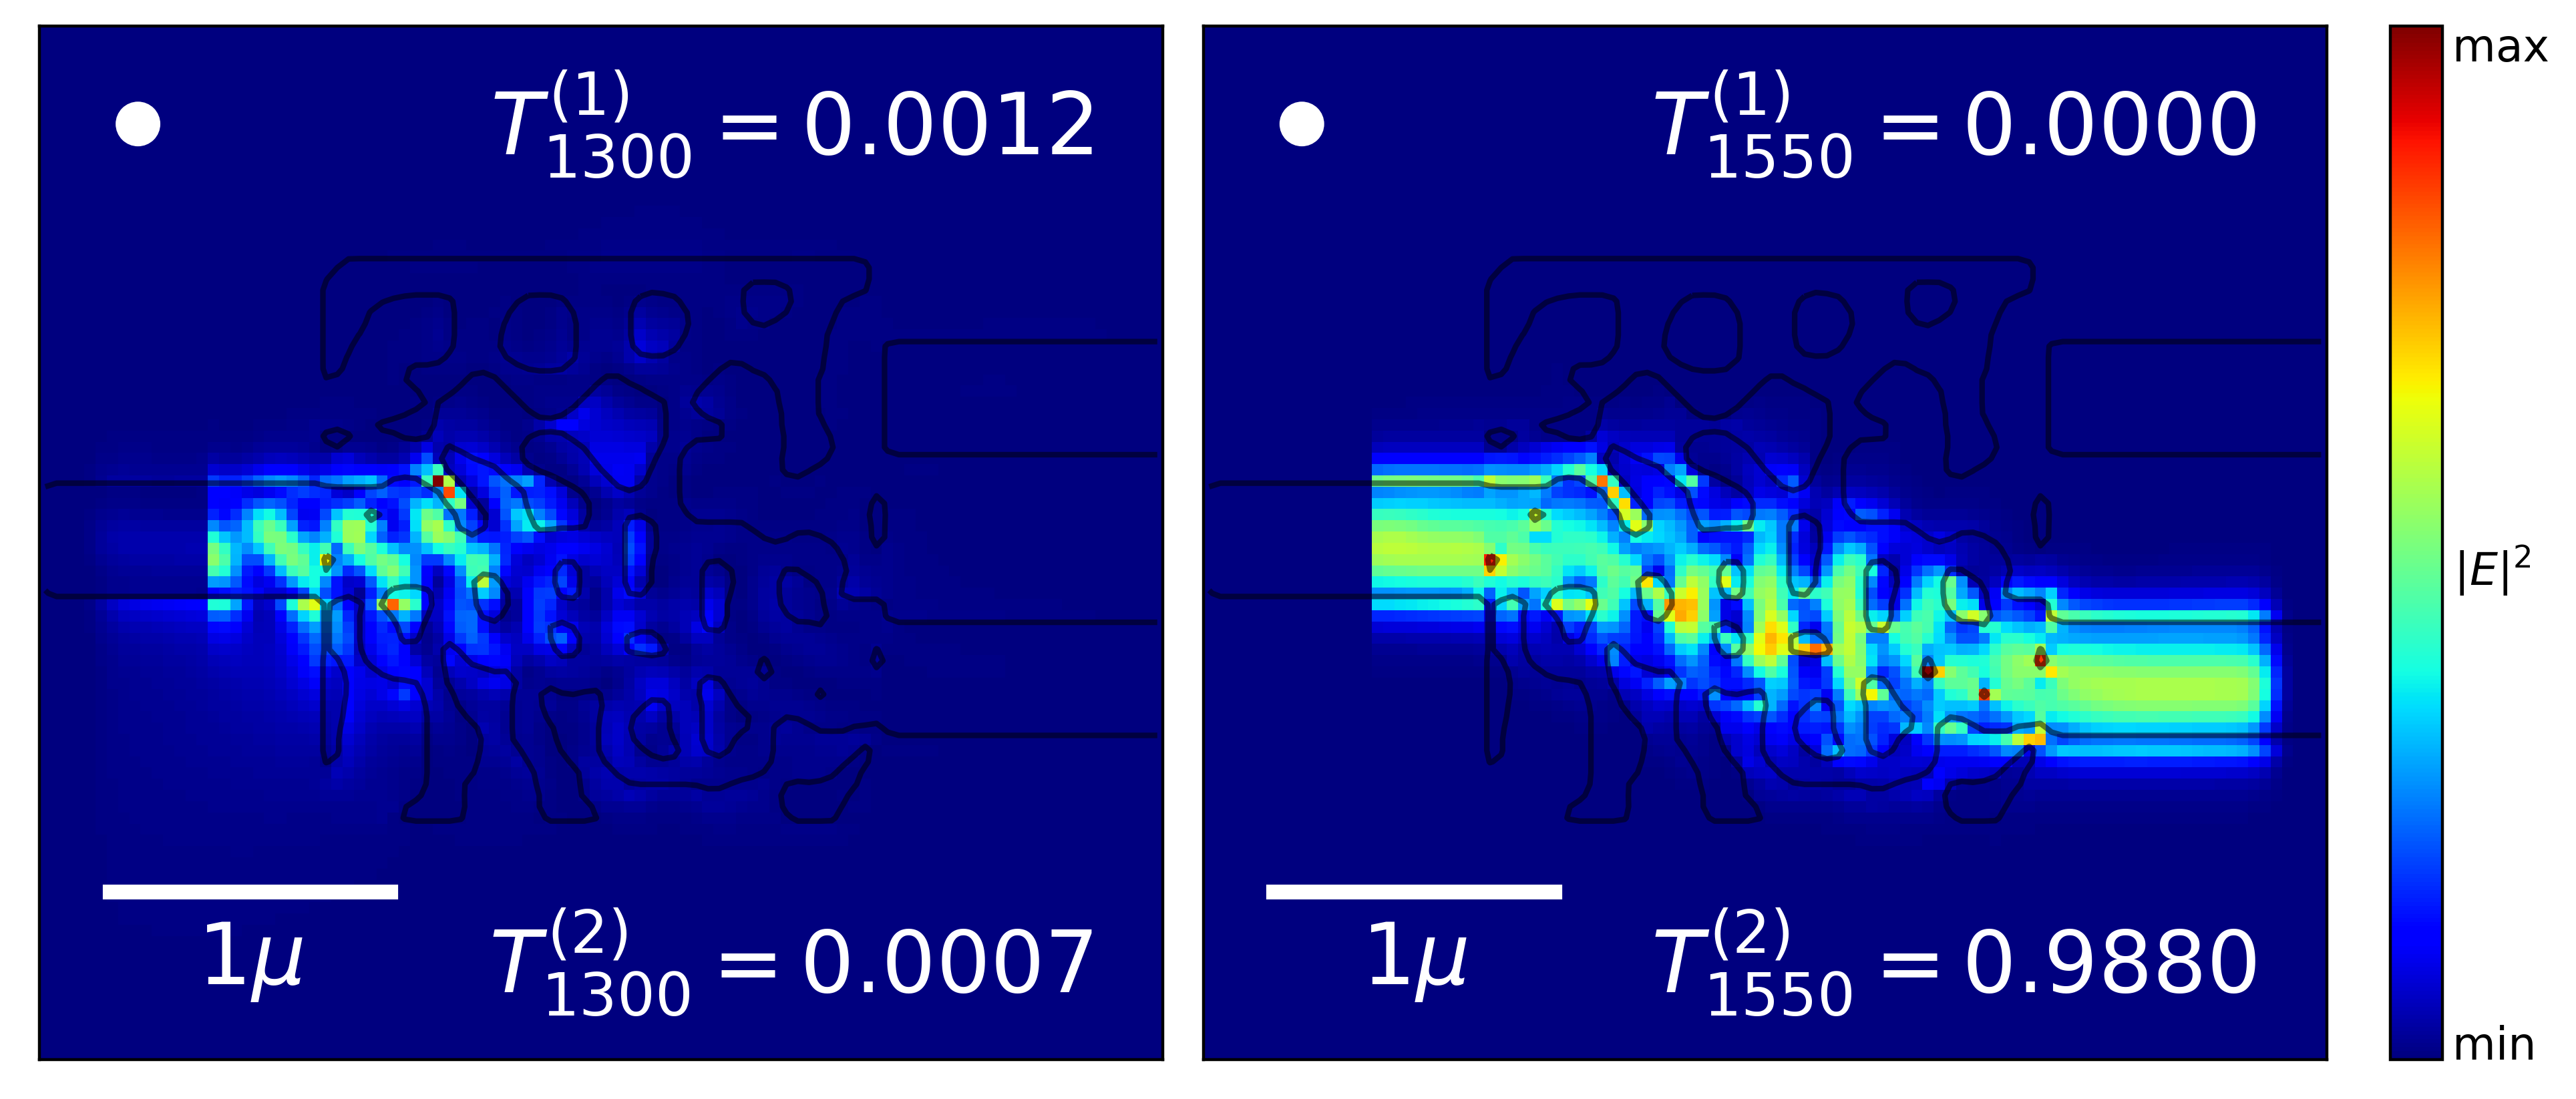
\includegraphics[width=0.50\textwidth]{image/results/wdm/L-BFGS-B/visualize_field_fab_256.png} \\
    \hline
      \multirow{2}{*}{512} &
      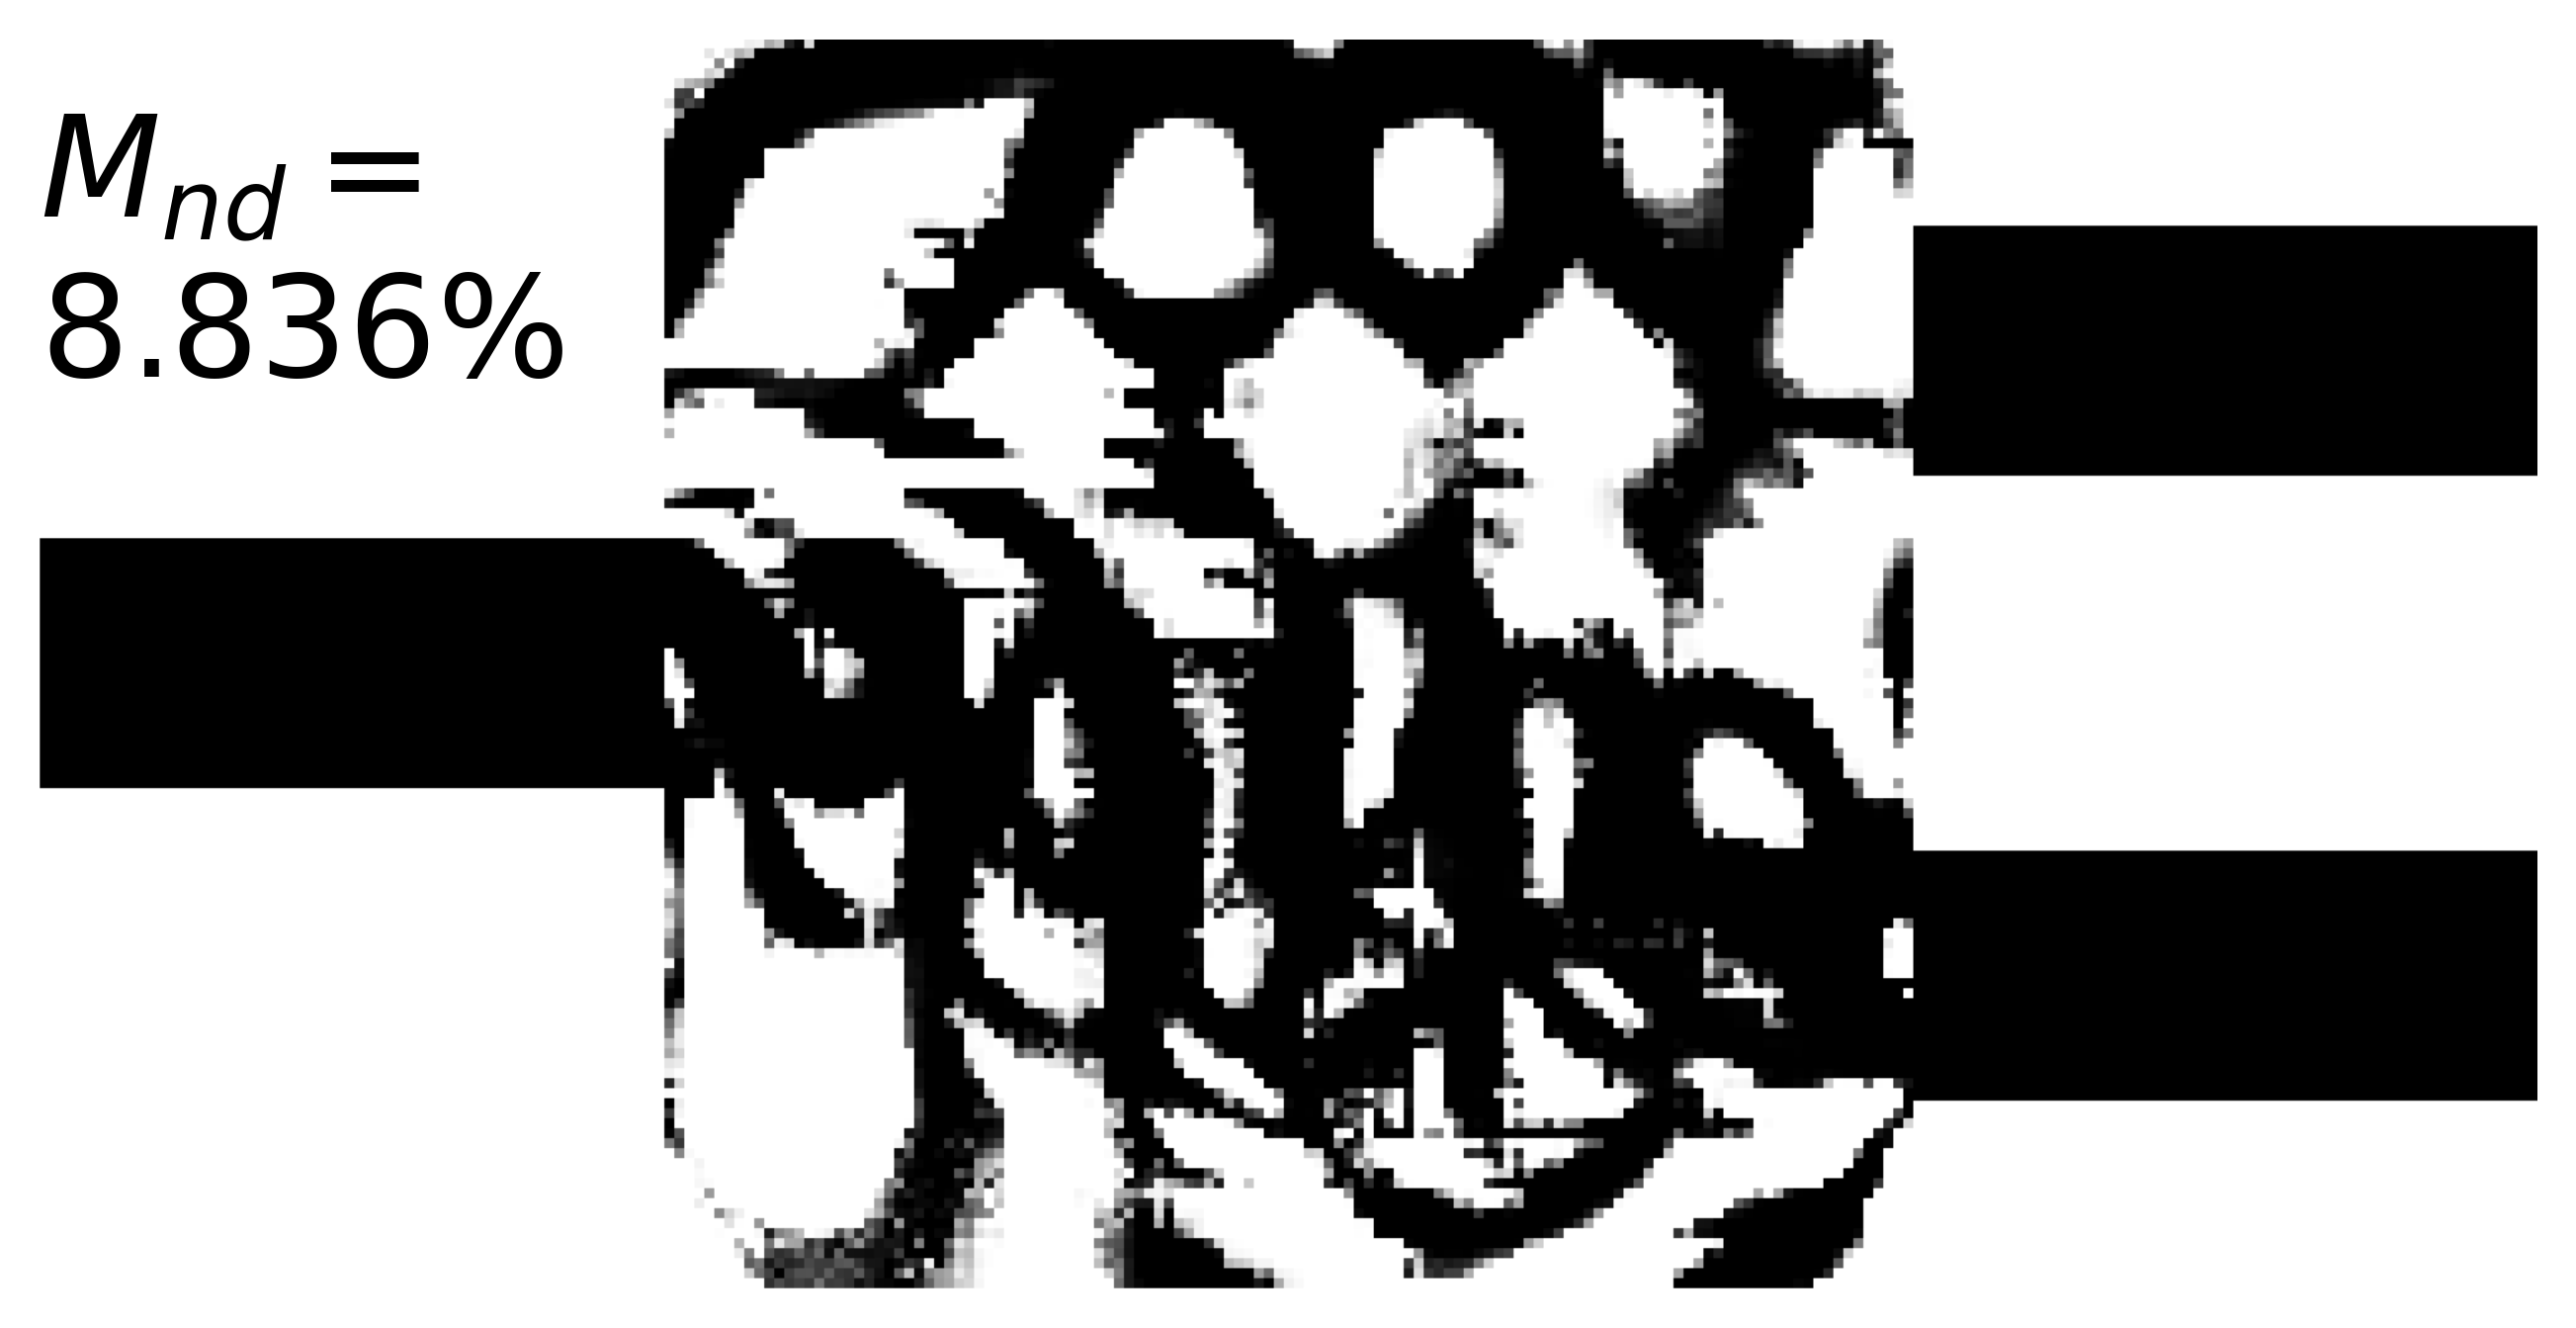
\includegraphics[width=0.24\textwidth]{image/results/wdm/L-BFGS-B/visualize_eps_cont_512.png} &
      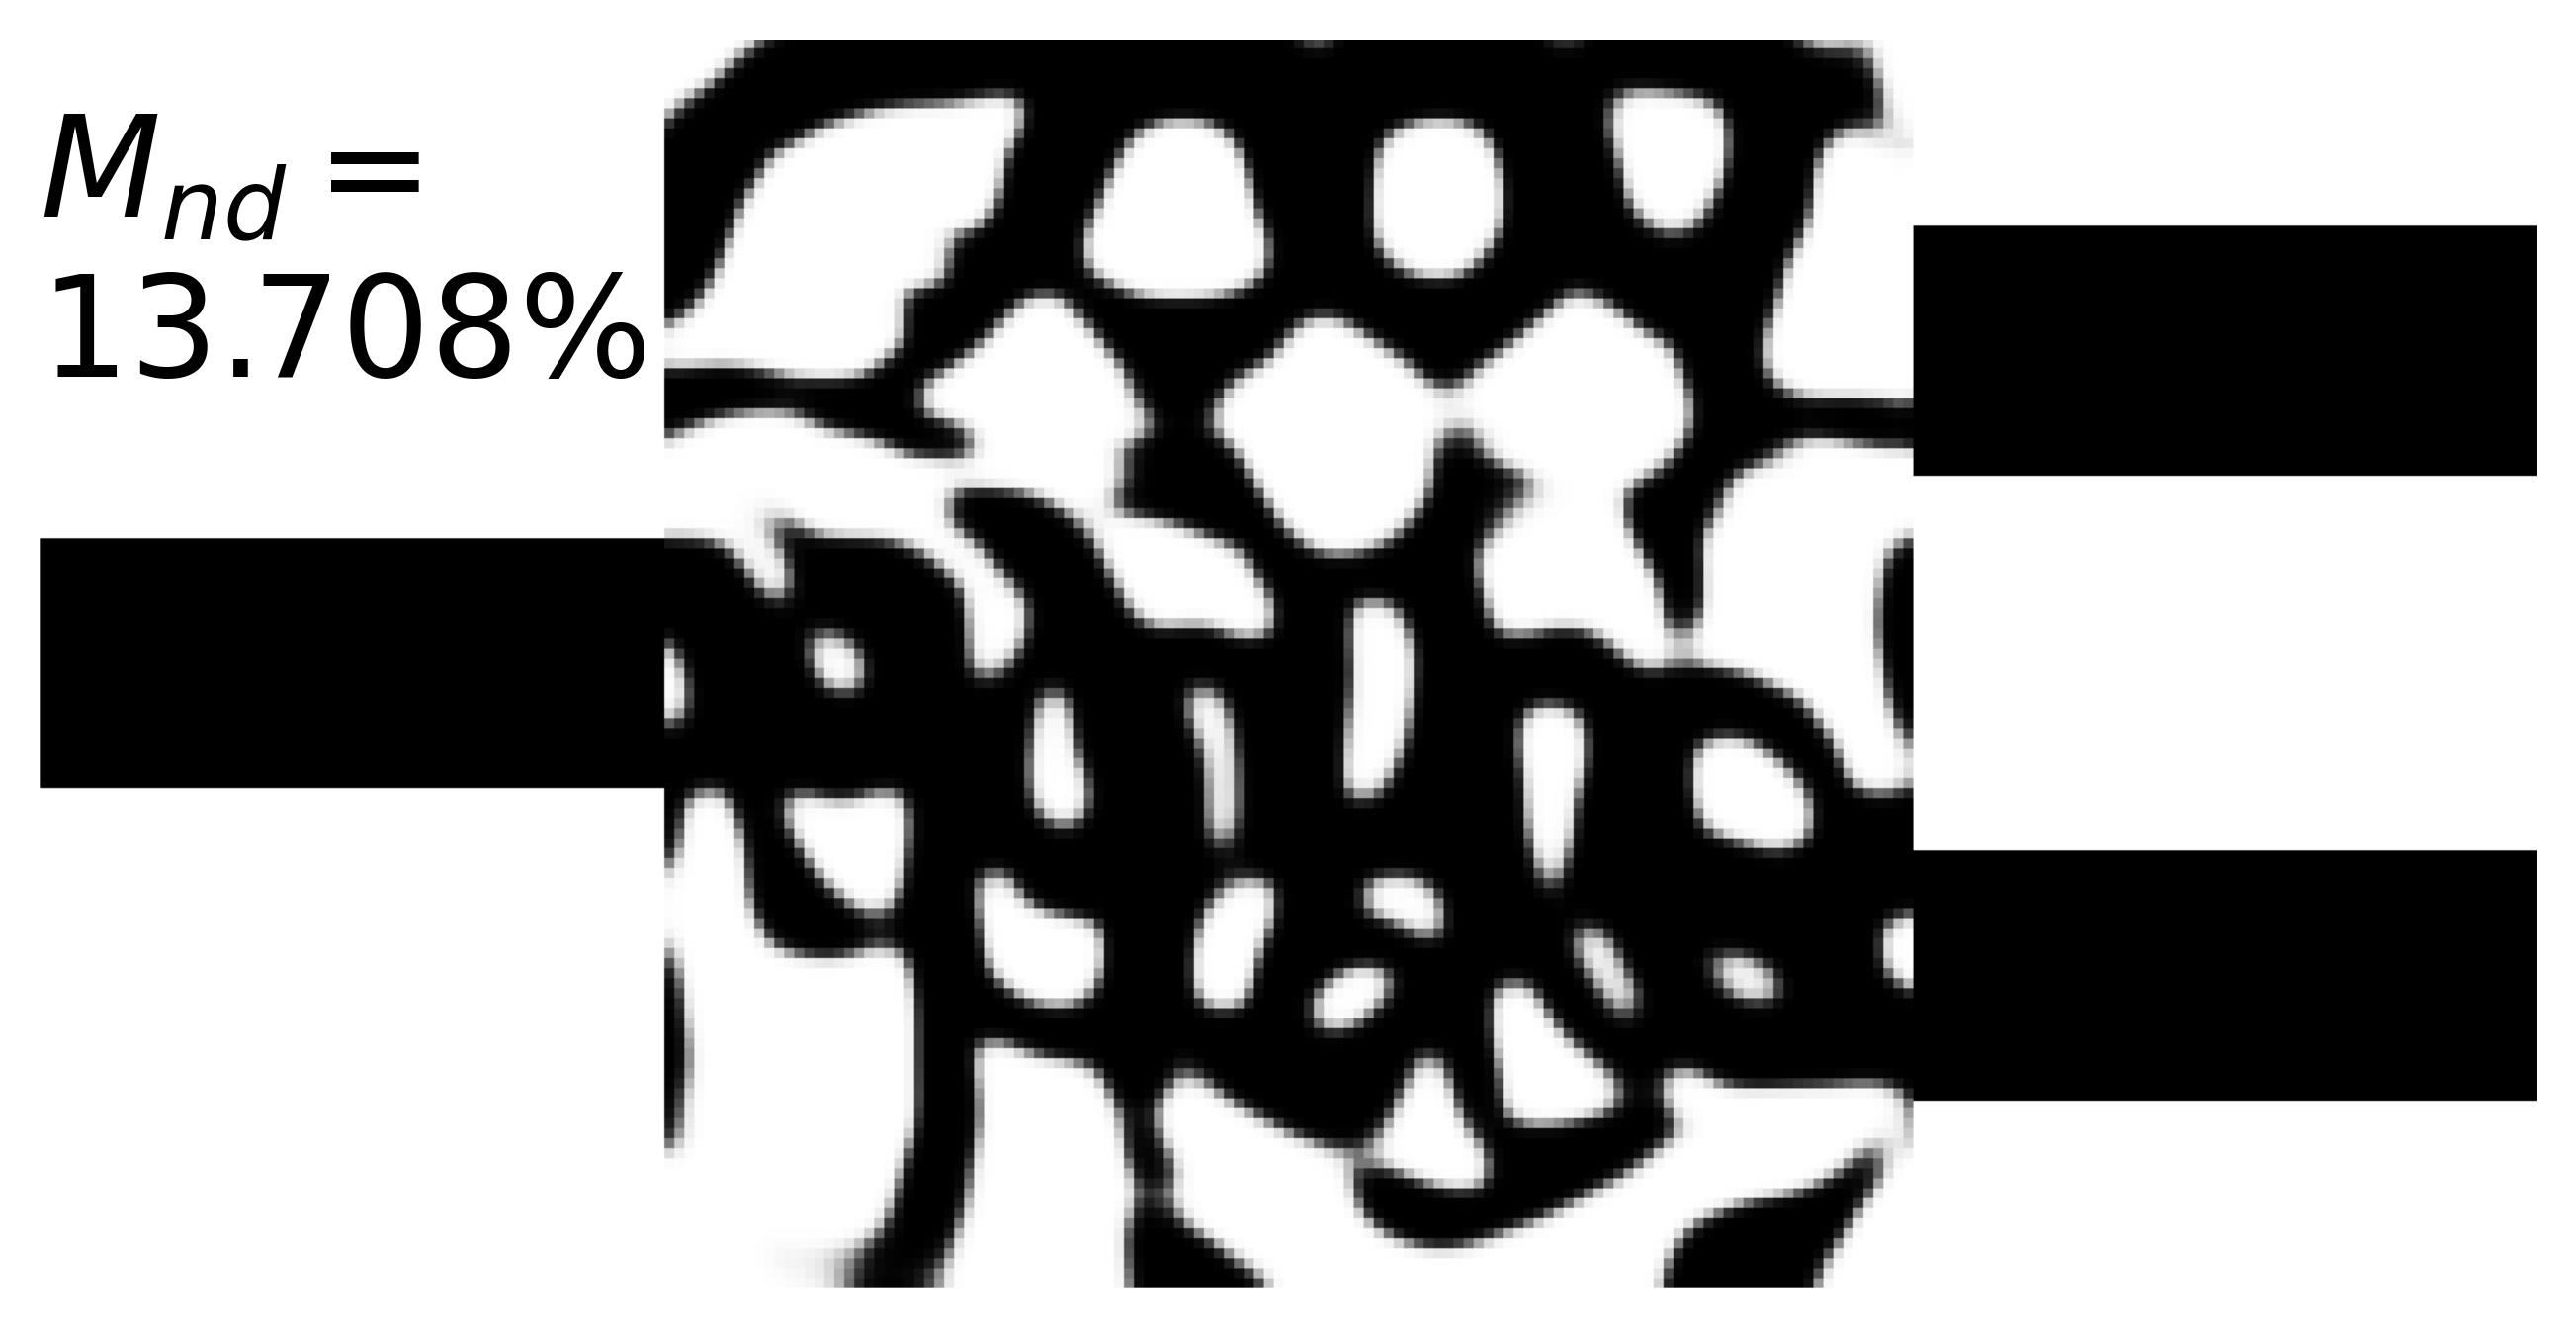
\includegraphics[width=0.24\textwidth]{image/results/wdm/L-BFGS-B/visualize_eps_disc_512.png} &
      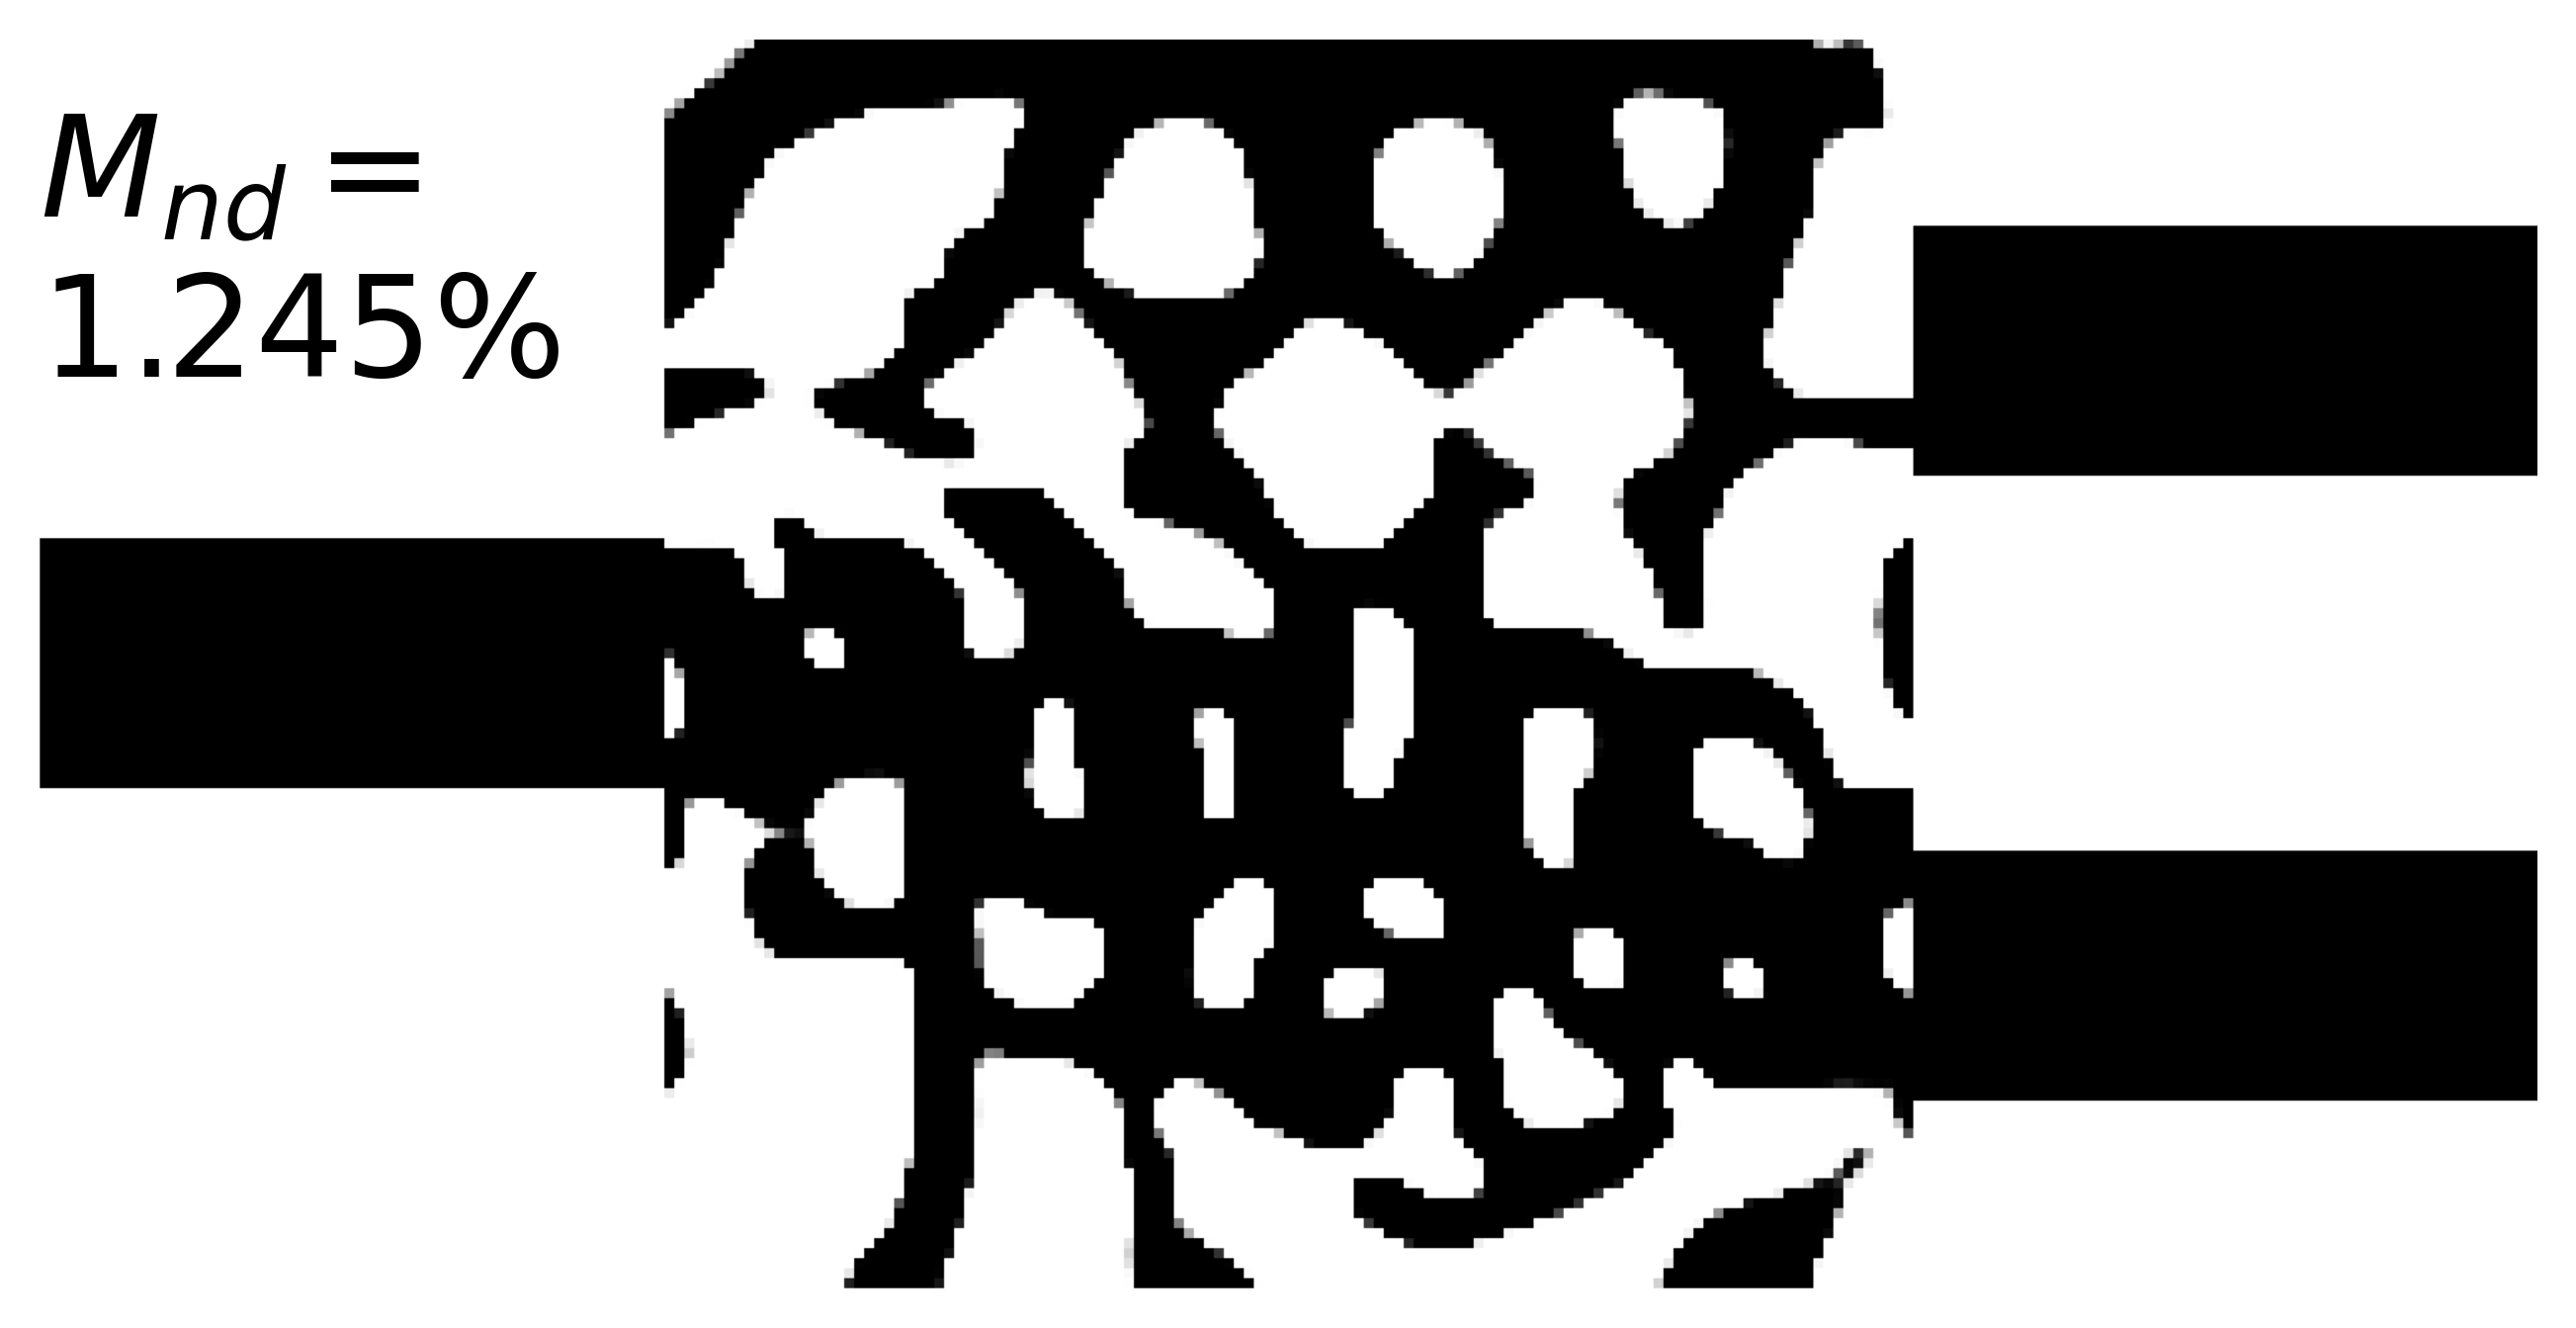
\includegraphics[width=0.24\textwidth]{image/results/wdm/L-BFGS-B/visualize_eps_fab_512.png} \\
      \cline{2-4}
      &
      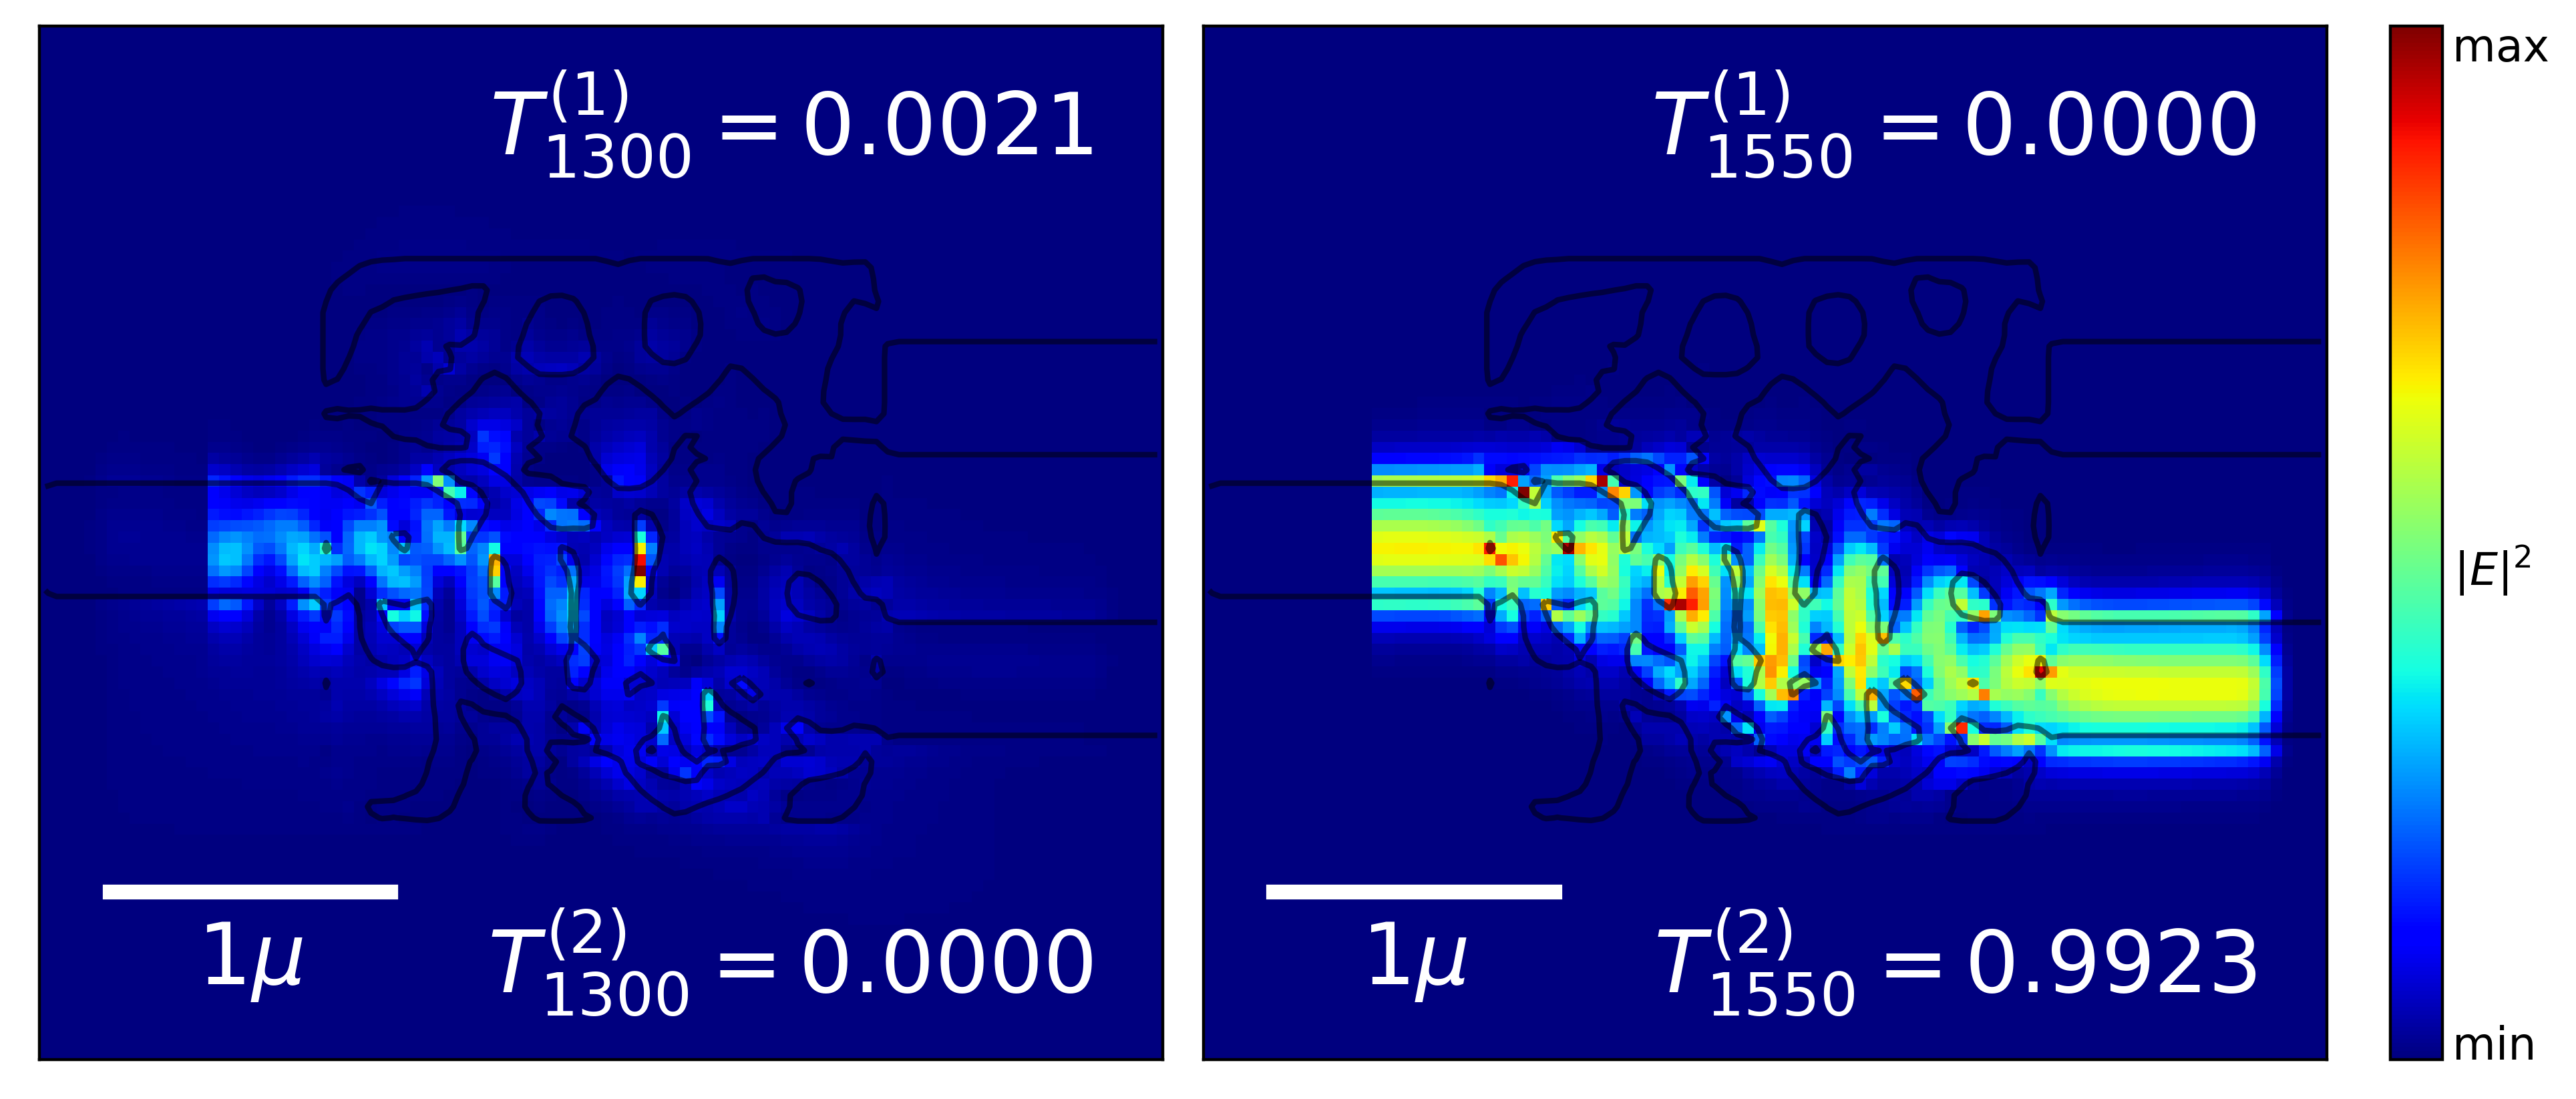
\includegraphics[width=0.50\textwidth]{image/results/wdm/L-BFGS-B/visualize_field_cont_512.png} &
      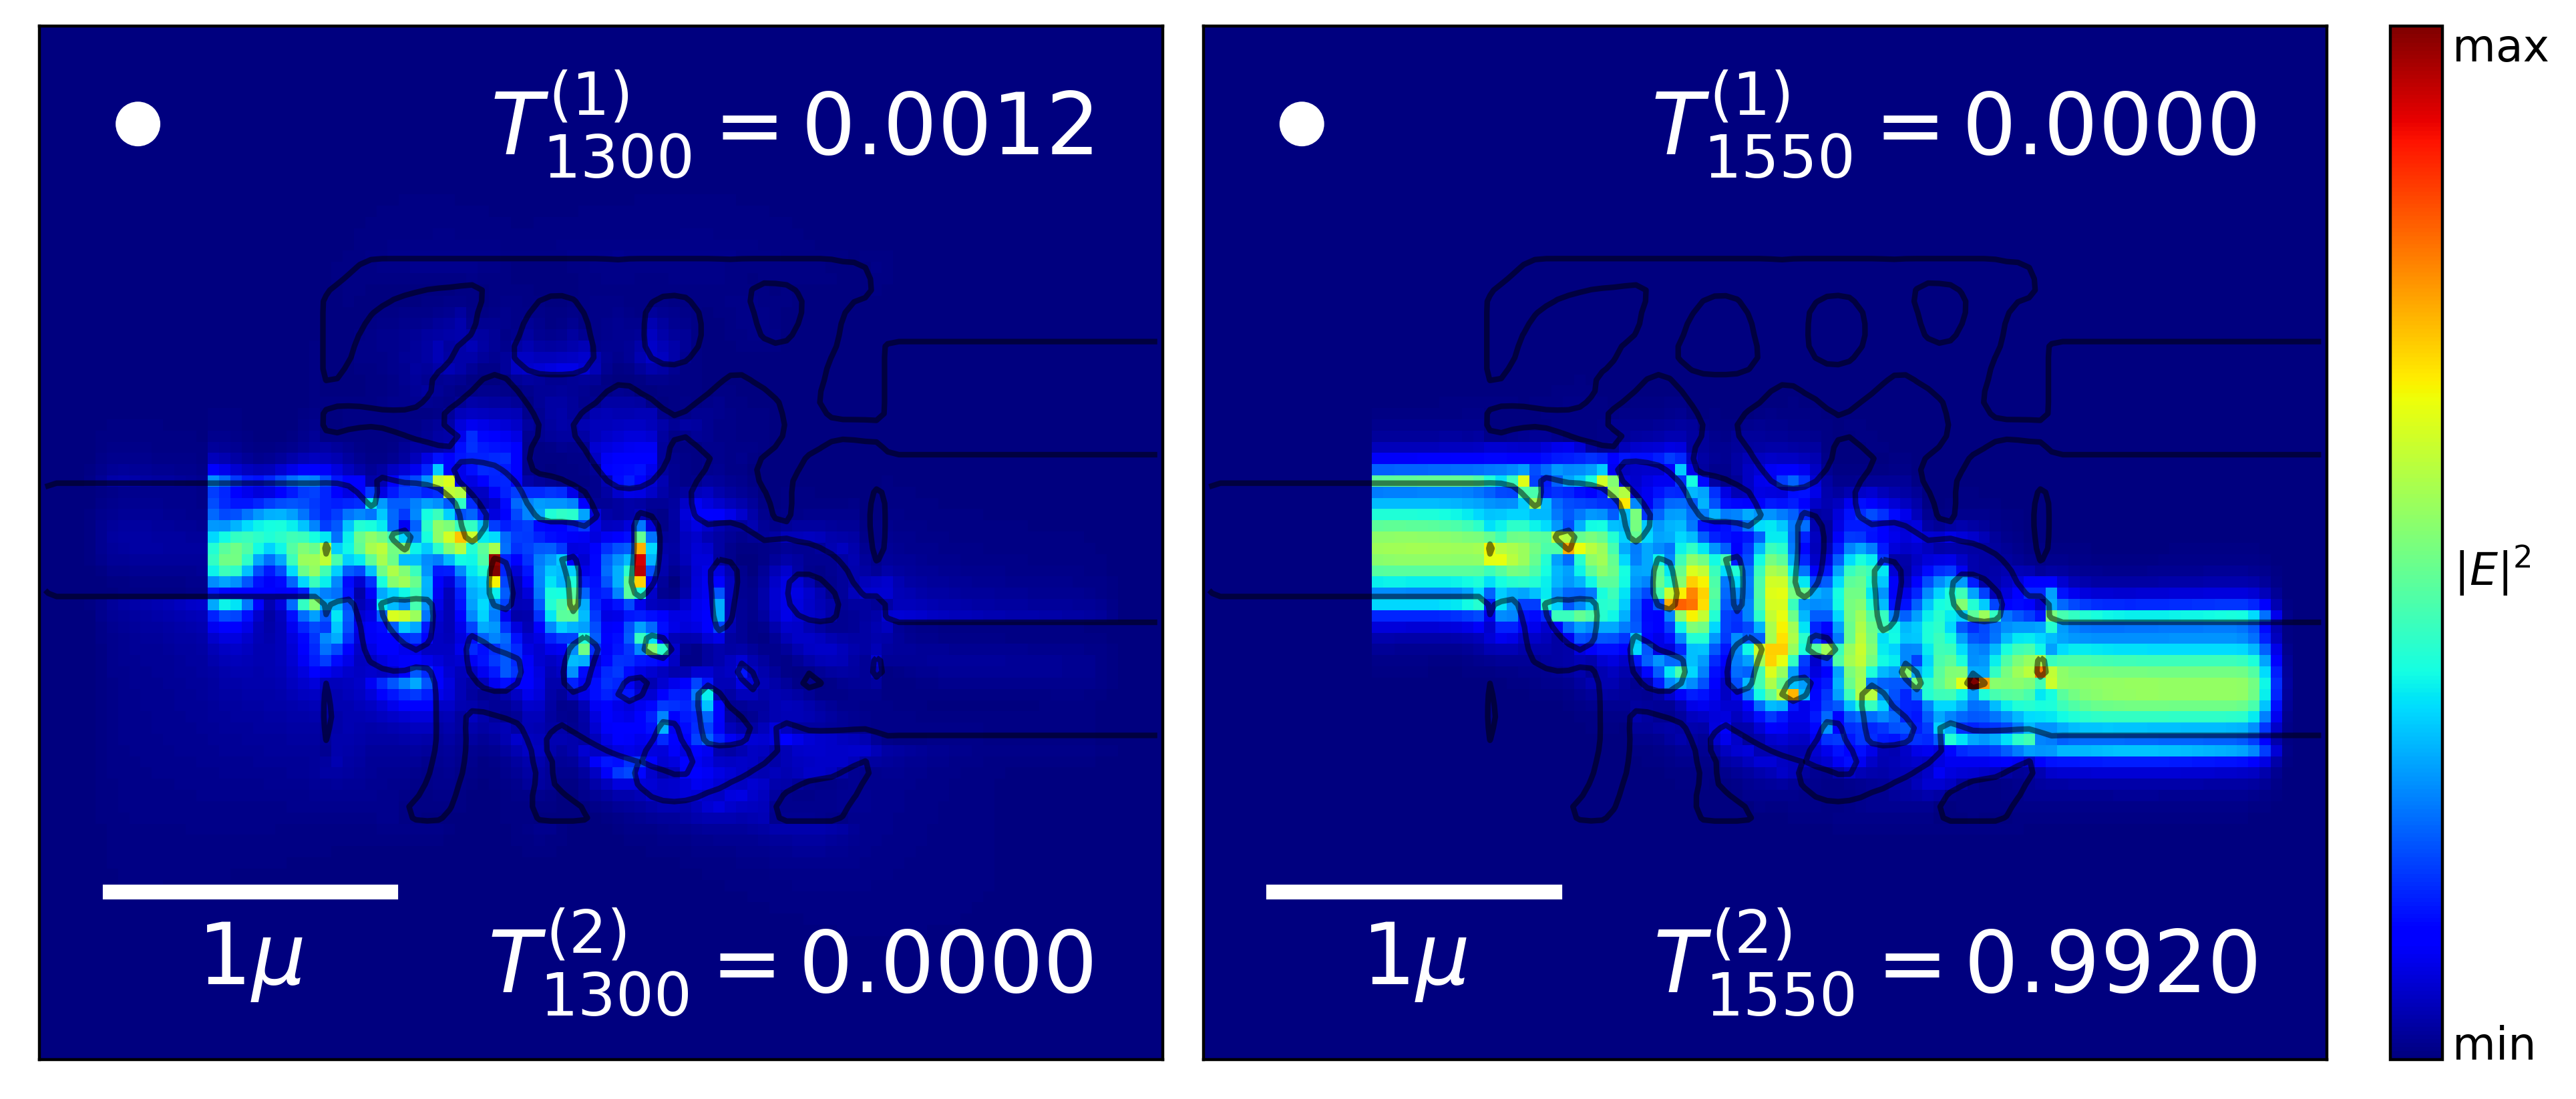
\includegraphics[width=0.50\textwidth]{image/results/wdm/L-BFGS-B/visualize_field_disc_512.png} &
      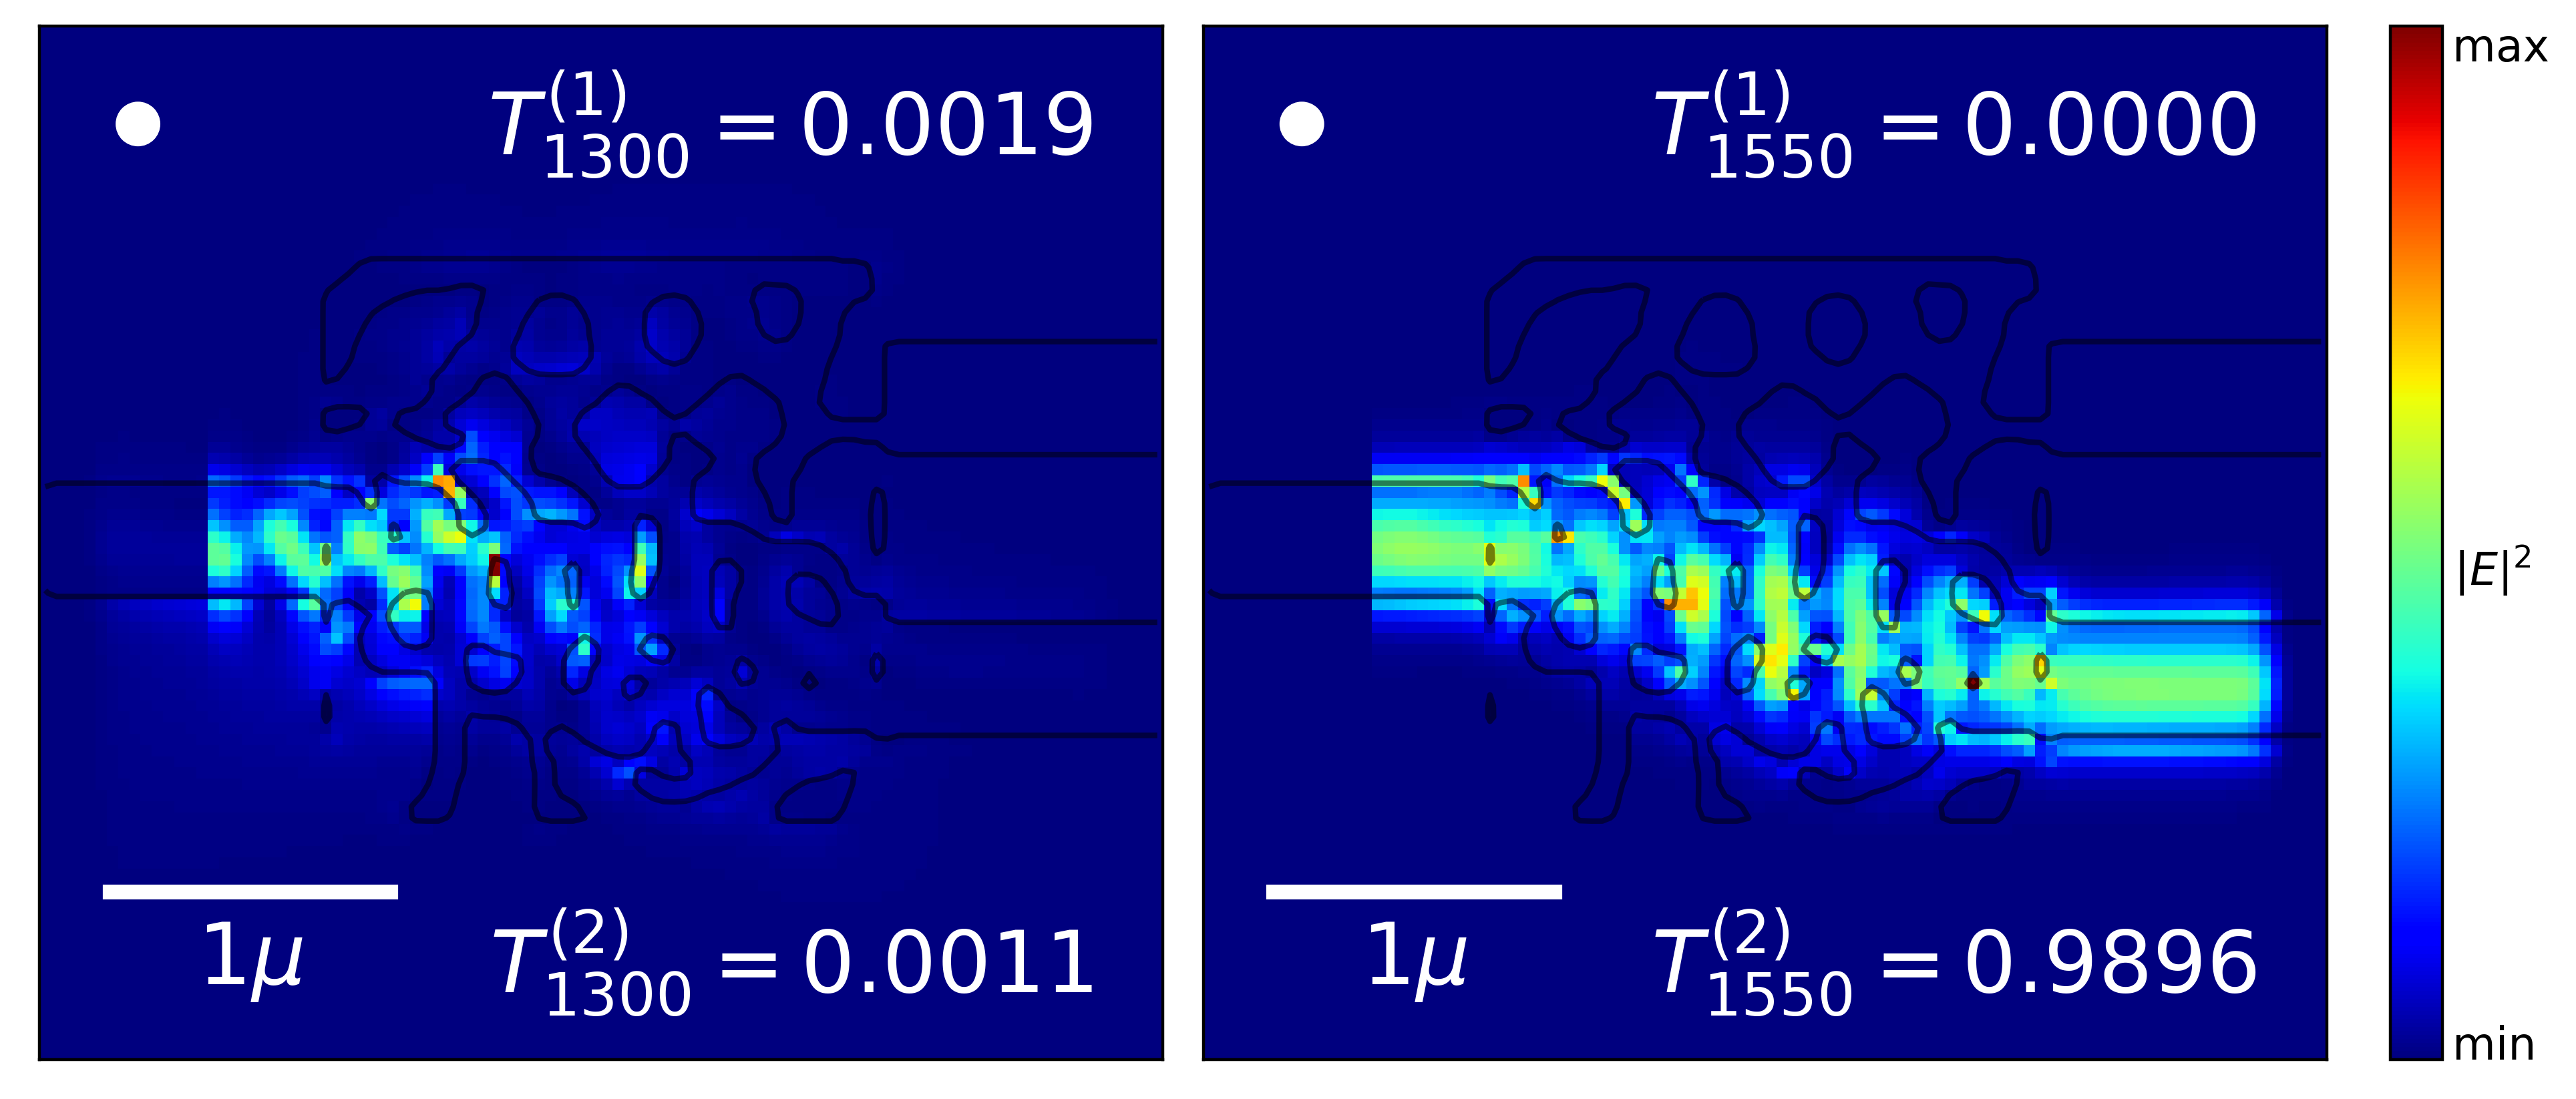
\includegraphics[width=0.50\textwidth]{image/results/wdm/L-BFGS-B/visualize_field_fab_512.png} \\
    \hline
    \end{tabular}
    \hspace*{-5cm}
    \caption{Resultados de la optimización continua al optimizar el WDM usando L-BFGS-B}
    \label{tab:opt-cont-L-BFGS-B-wdm}
\end{table}
\end{landscape}


% Best - Bend - L-BFGS-B
\begin{table}[ht]
    \centering
    \hspace*{-3cm}
    \begin{tabular}{|c|c|c|}
    \hline
      $\eta_d = 0.45$ &
      
\includegraphics[width=0.40\textwidth]{image/results/bend/L-BFGS-B/best/eps_eta_d_256.png } &
      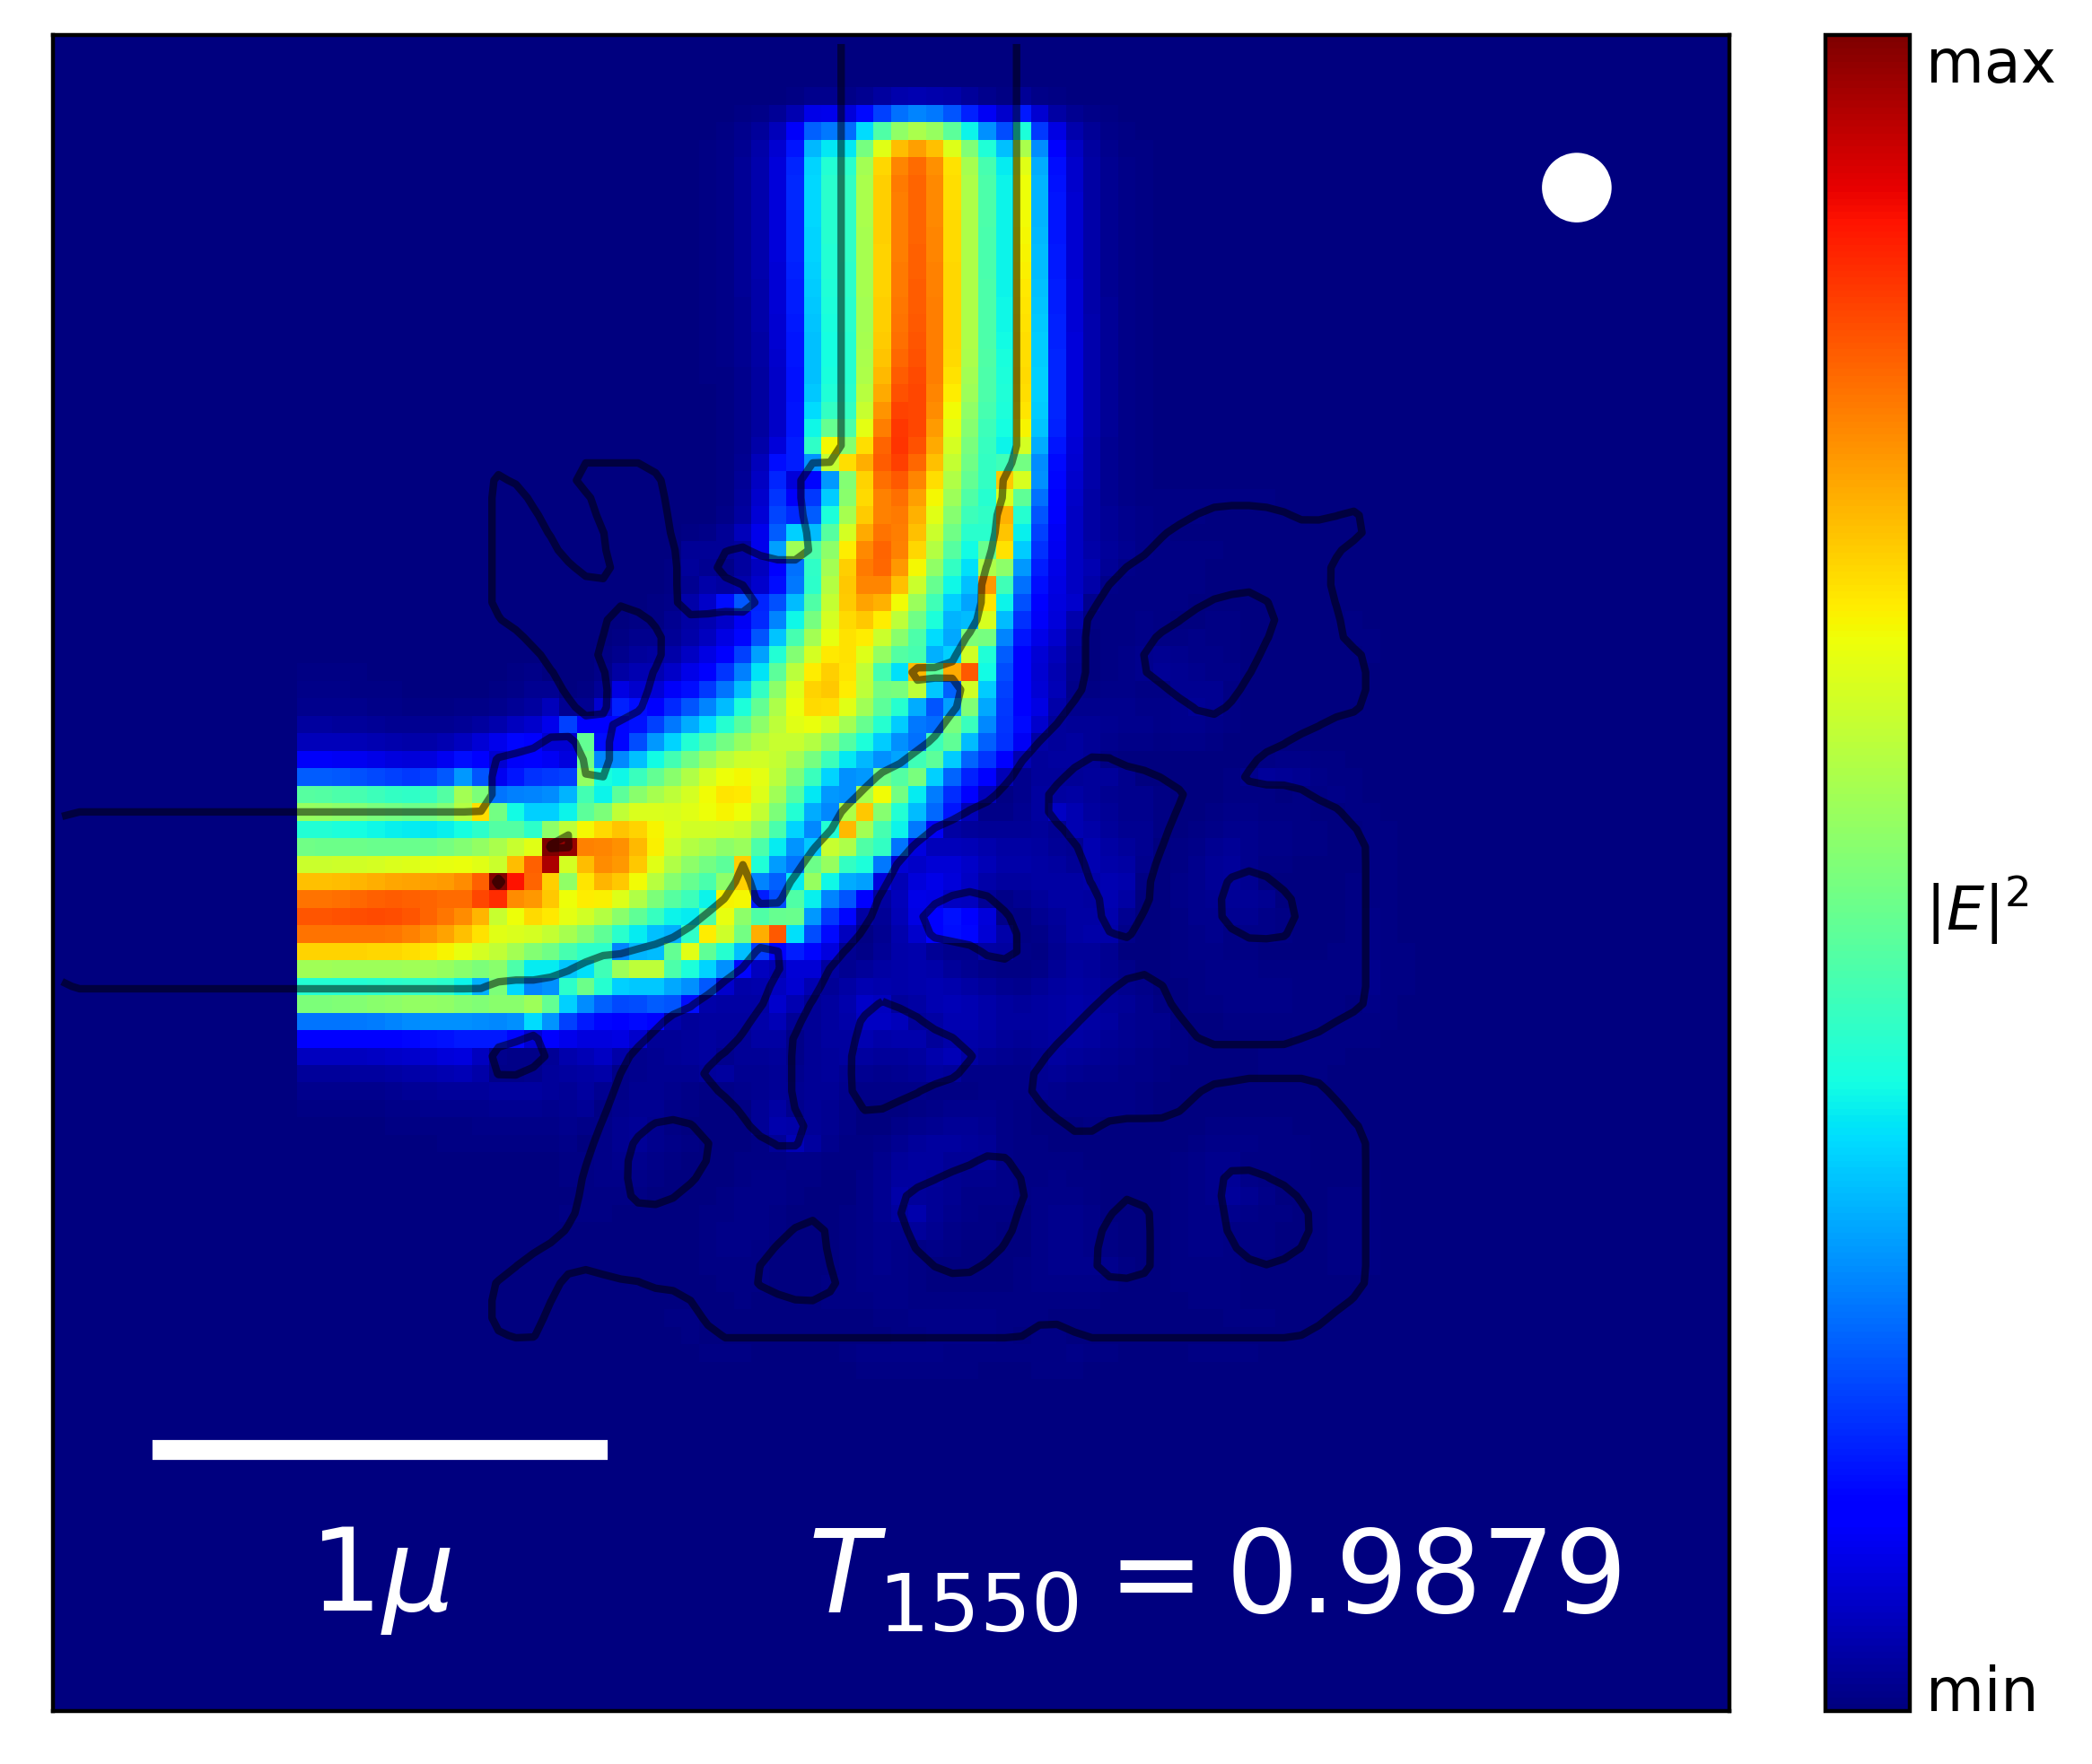
\includegraphics[width=0.50\textwidth]{image/results/bend/L-BFGS-B/best/field_eta_d_256.png} \\
    \hline
      $\eta_i = 0.50$ &
      
\includegraphics[width=0.40\textwidth]{image/results/bend/L-BFGS-B/best/eps_eta_i_256.png} &
      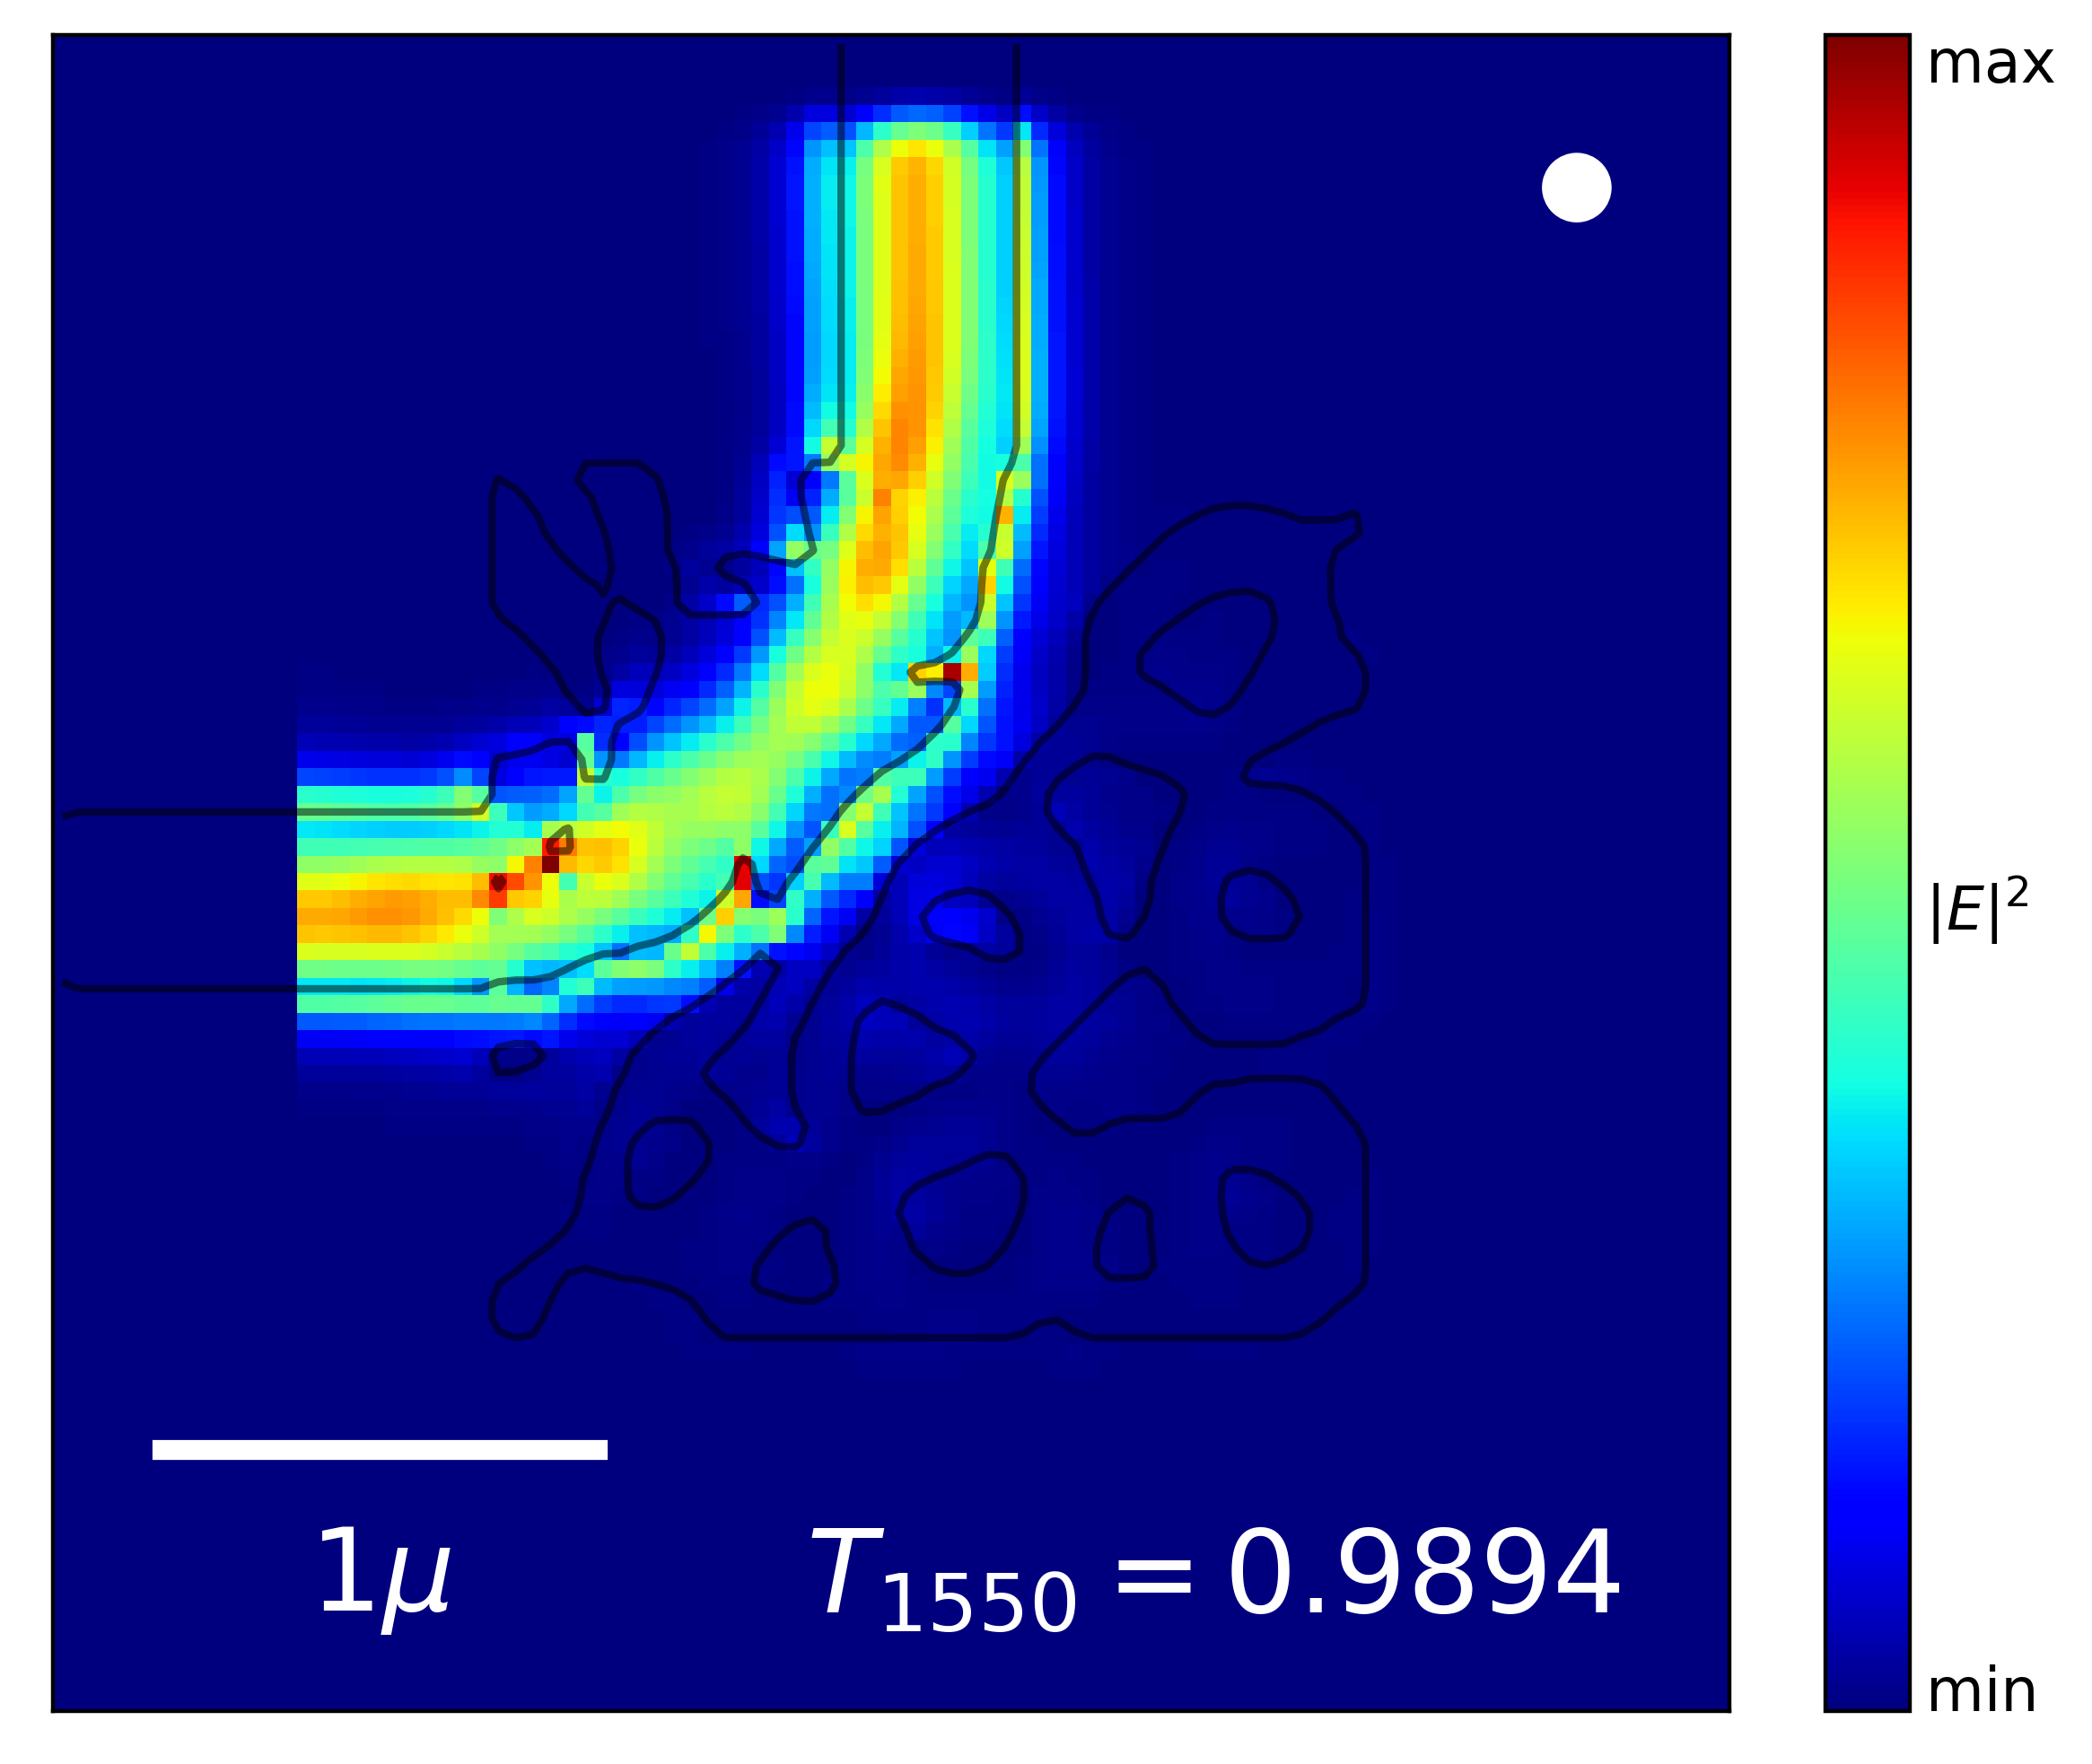
\includegraphics[width=0.50\textwidth]{image/results/bend/L-BFGS-B/best/field_eta_i_256.png} \\
    \hline
      $\eta_e = 0.55$ &
      
\includegraphics[width=0.40\textwidth]{image/results/bend/L-BFGS-B/best/eps_eta_e_256.png} &
      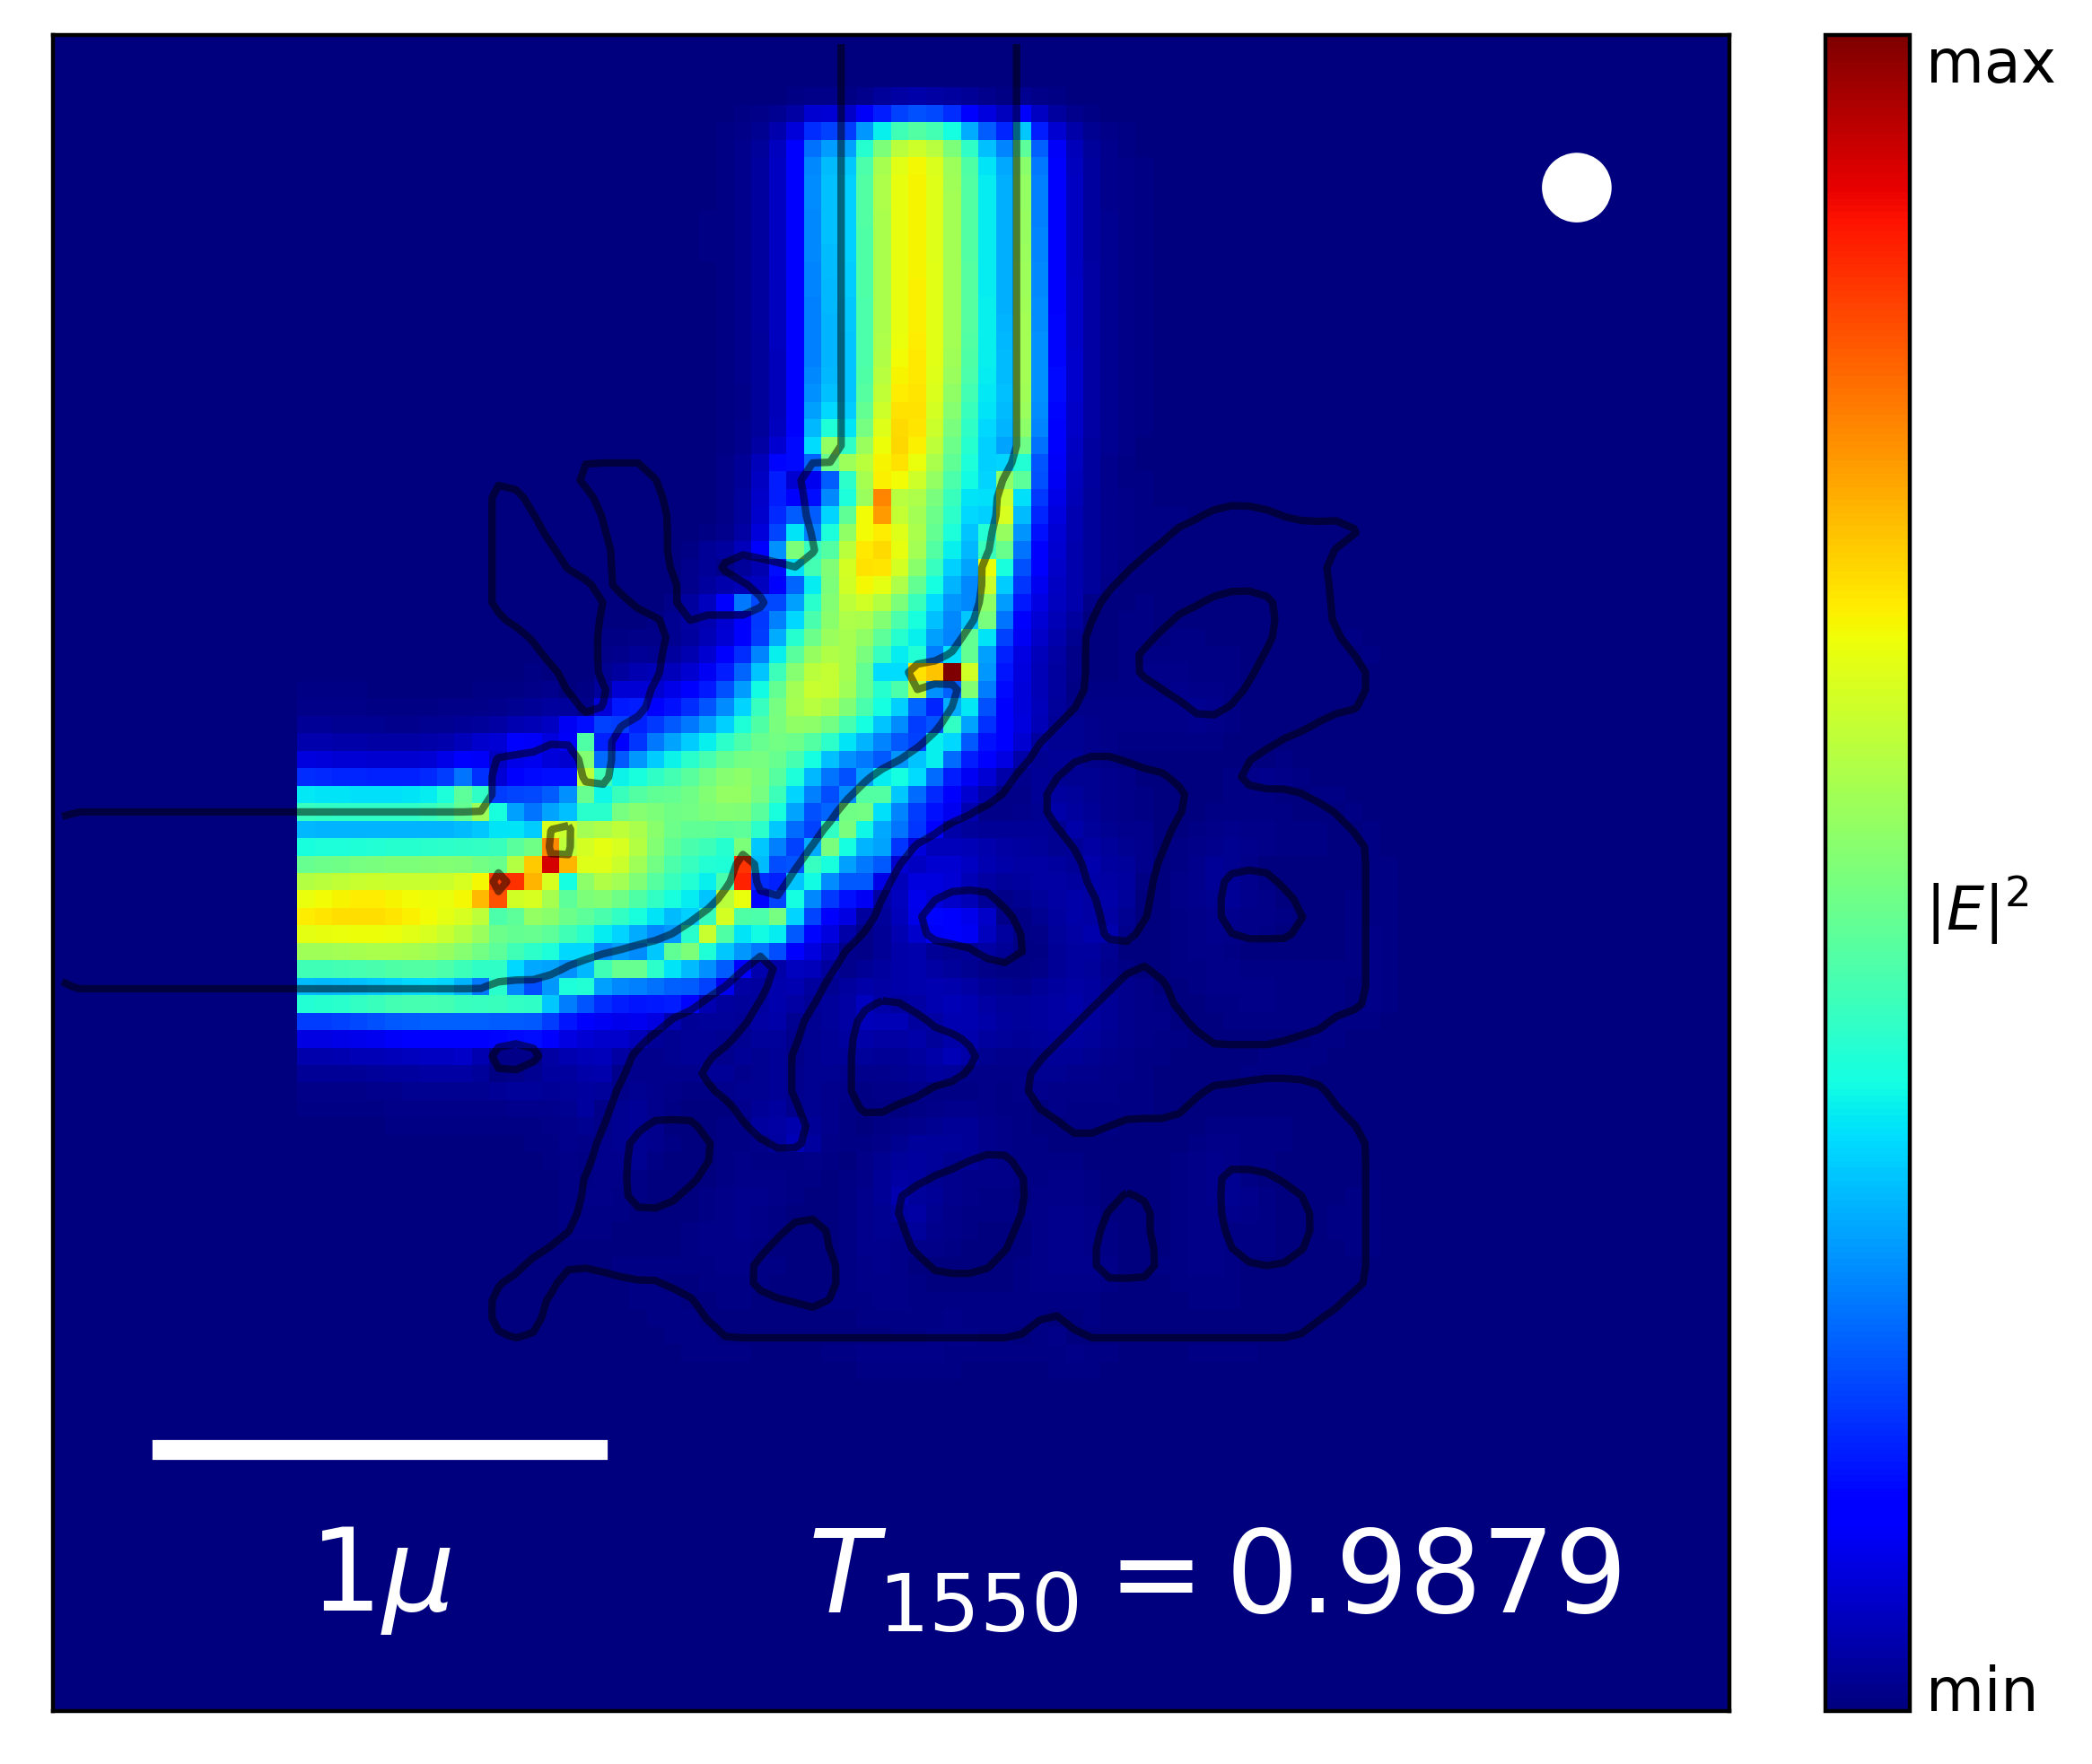
\includegraphics[width=0.50\textwidth]{image/results/bend/L-BFGS-B/best/field_eta_e_256.png} \\
    \hline
    \end{tabular}
    \hspace*{-3cm}
    \caption{Mejores diseños del \emph{bend} usando L-BFGS-B  ($seed = 256$).
    Las imágenes de la primera fila corresponden al diseño dilatado ($\eta_d$), 
    las de la segunda fila al diseño nominal ($\eta_i$) y la tercera fila al diseño erosionado ($\eta_e$).}
    \label{tab:best-bend-L-BFGS-B}
\end{table}


% Best - WDM - L-BFGS-B
\begin{table}[ht]
    \centering
    \hspace*{-3cm}
    \begin{tabular}{|c|c|c|}
    \hline
      $\eta_d = 0.45$ &
      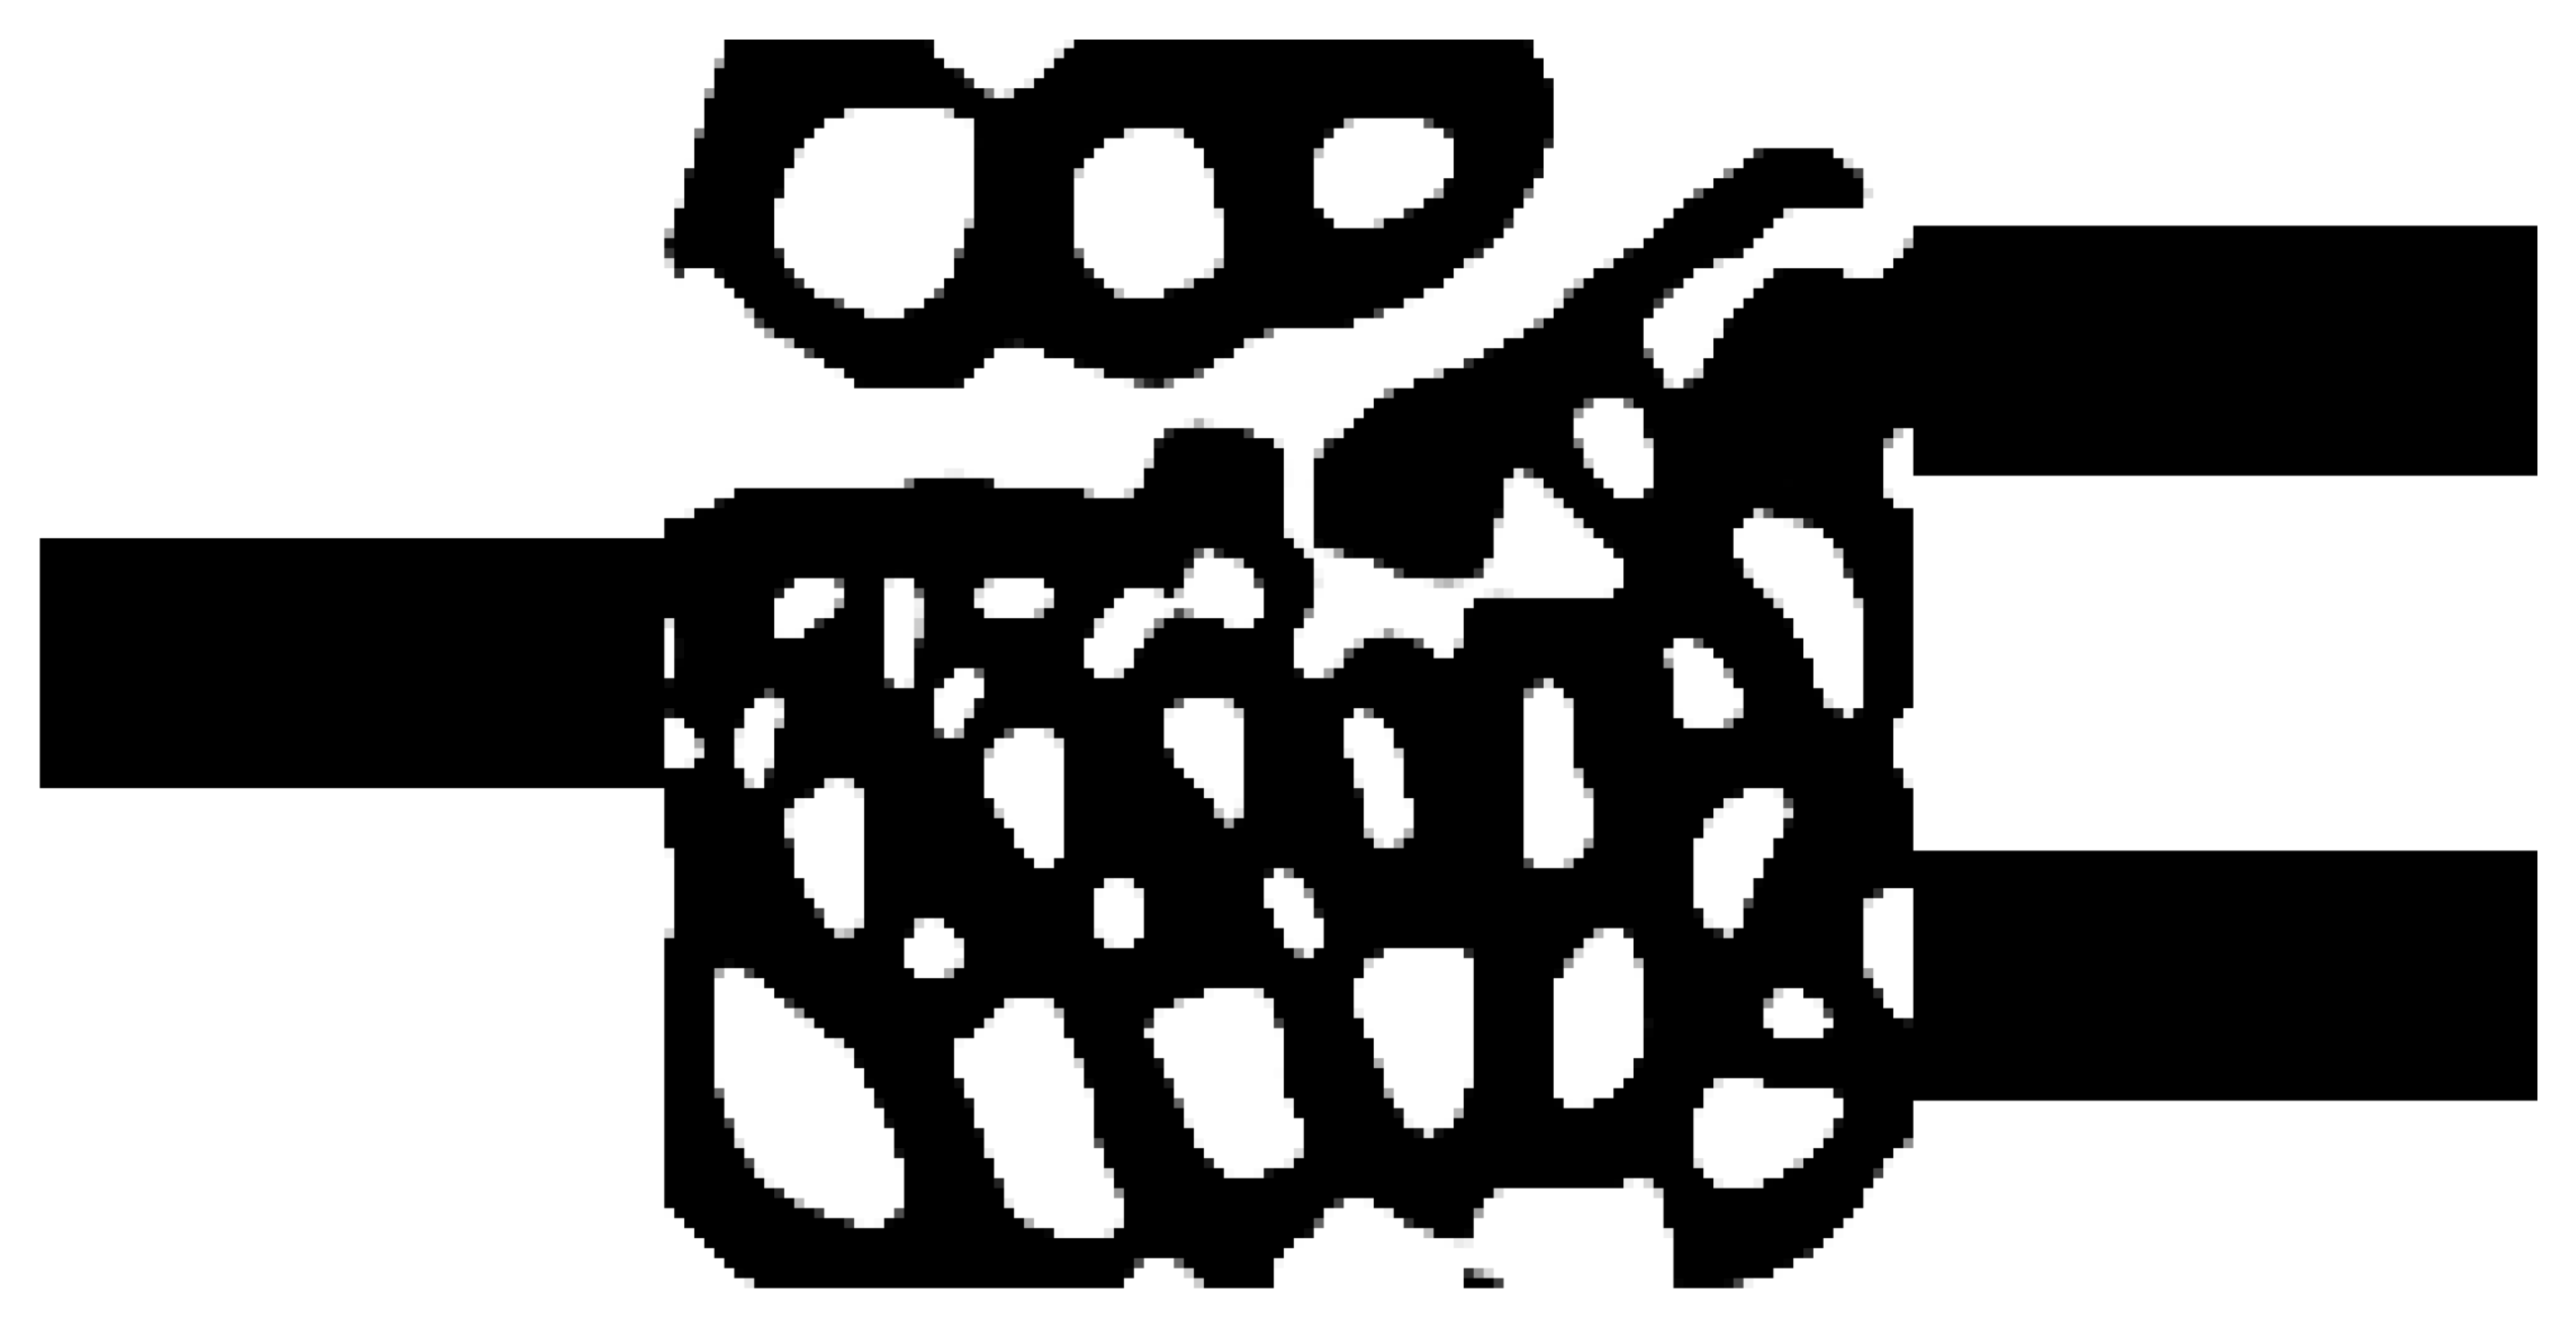
\includegraphics[width=0.35\textwidth]{image/results/wdm/L-BFGS-B/best/eps_eta_d_128.png } &
      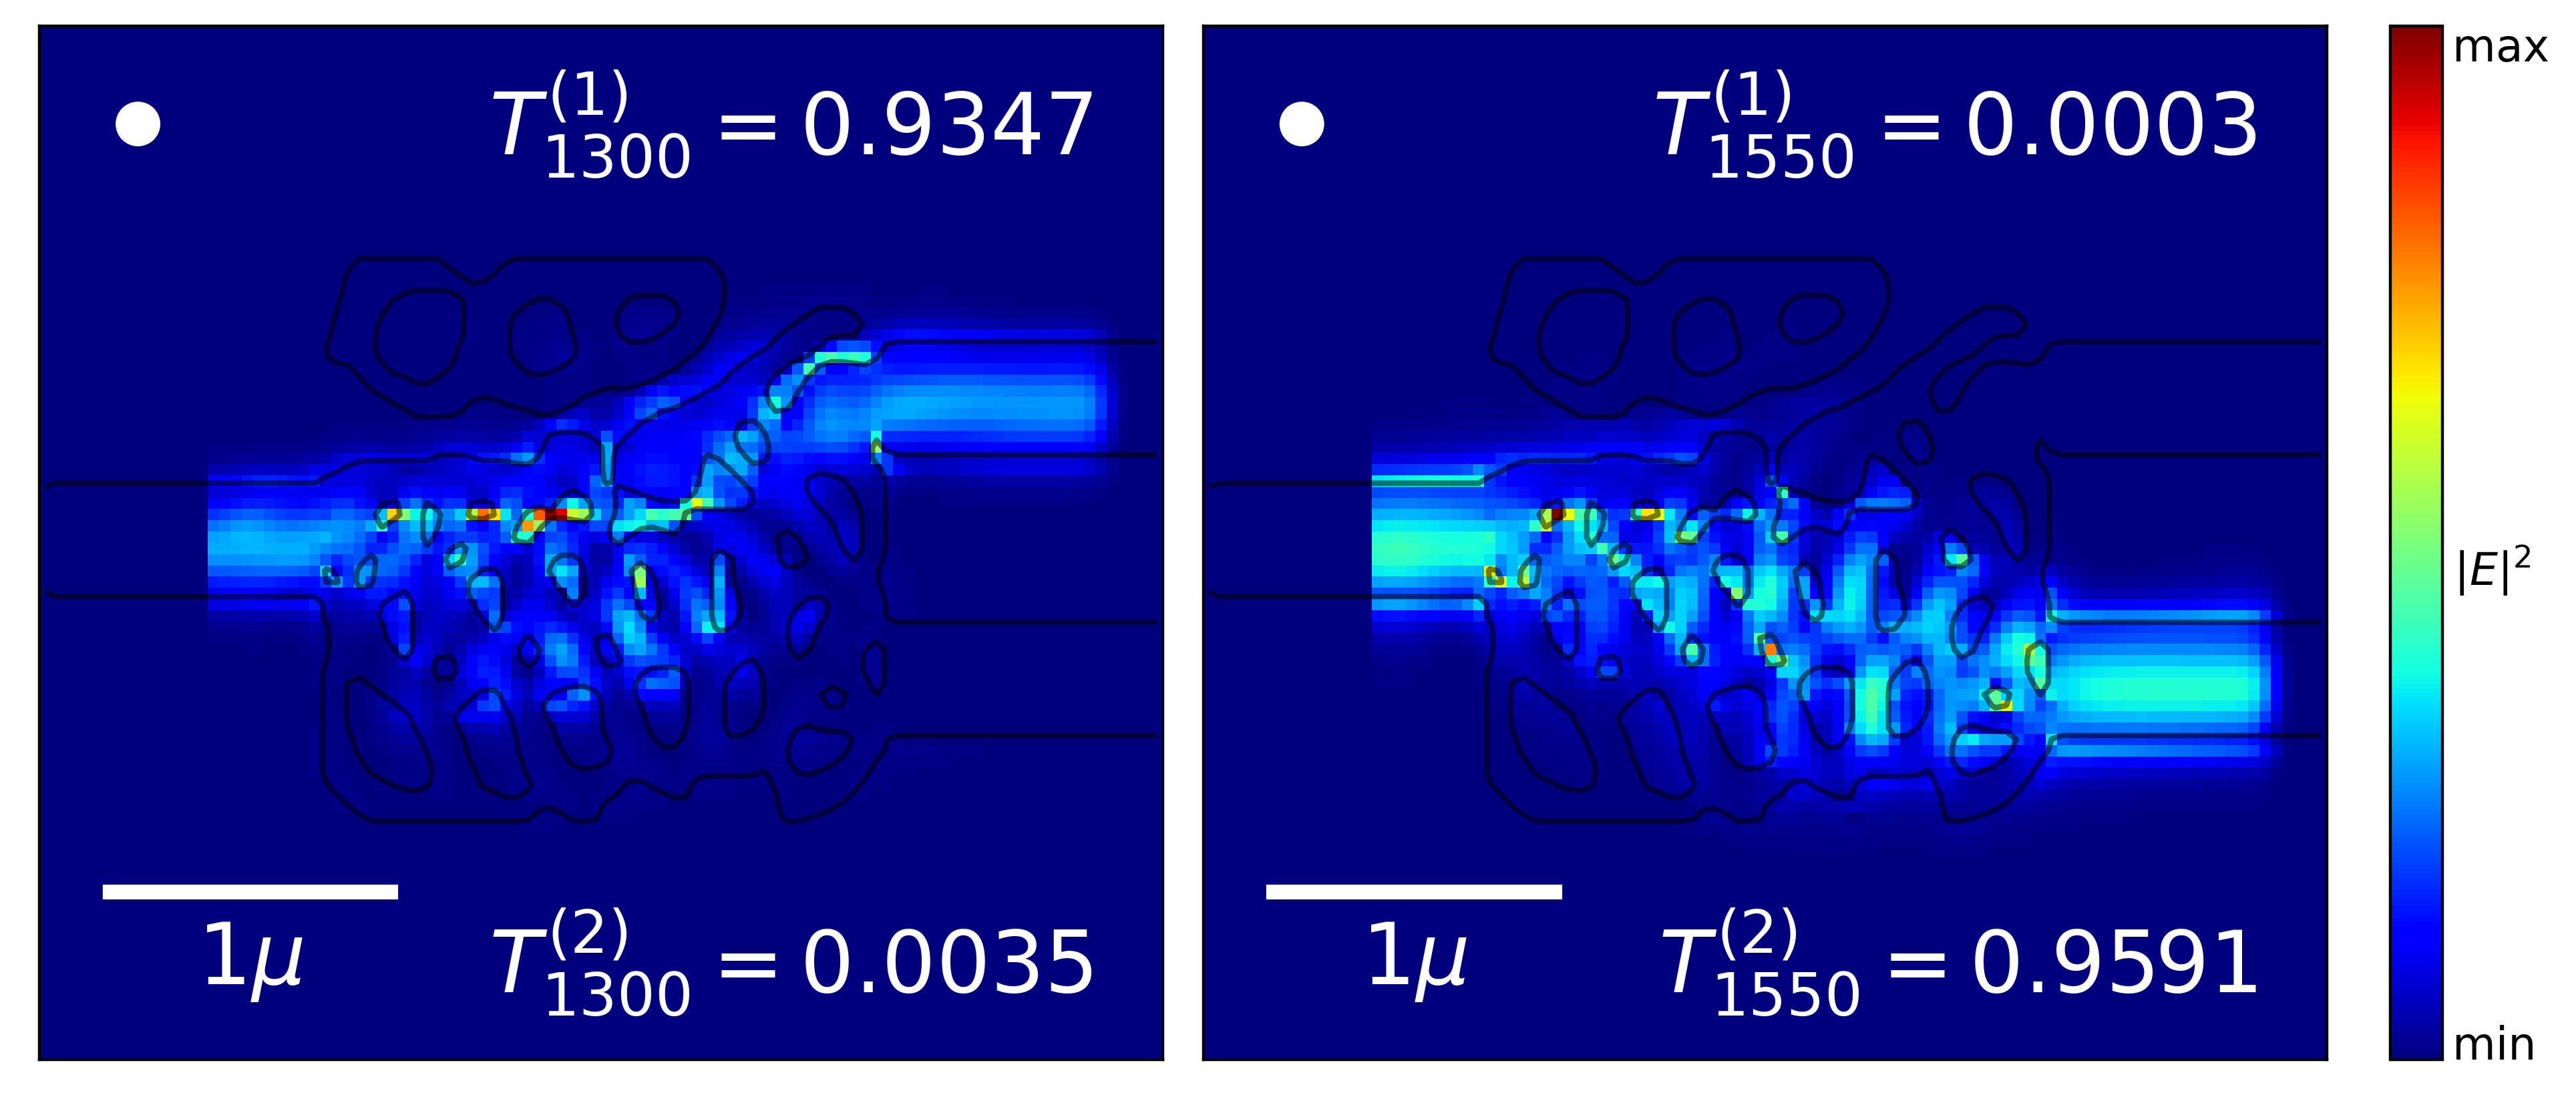
\includegraphics[width=0.60\textwidth]{image/results/wdm/L-BFGS-B/best/field_eta_d_128.png} \\
    \hline
      $\eta_i = 0.50$ &
      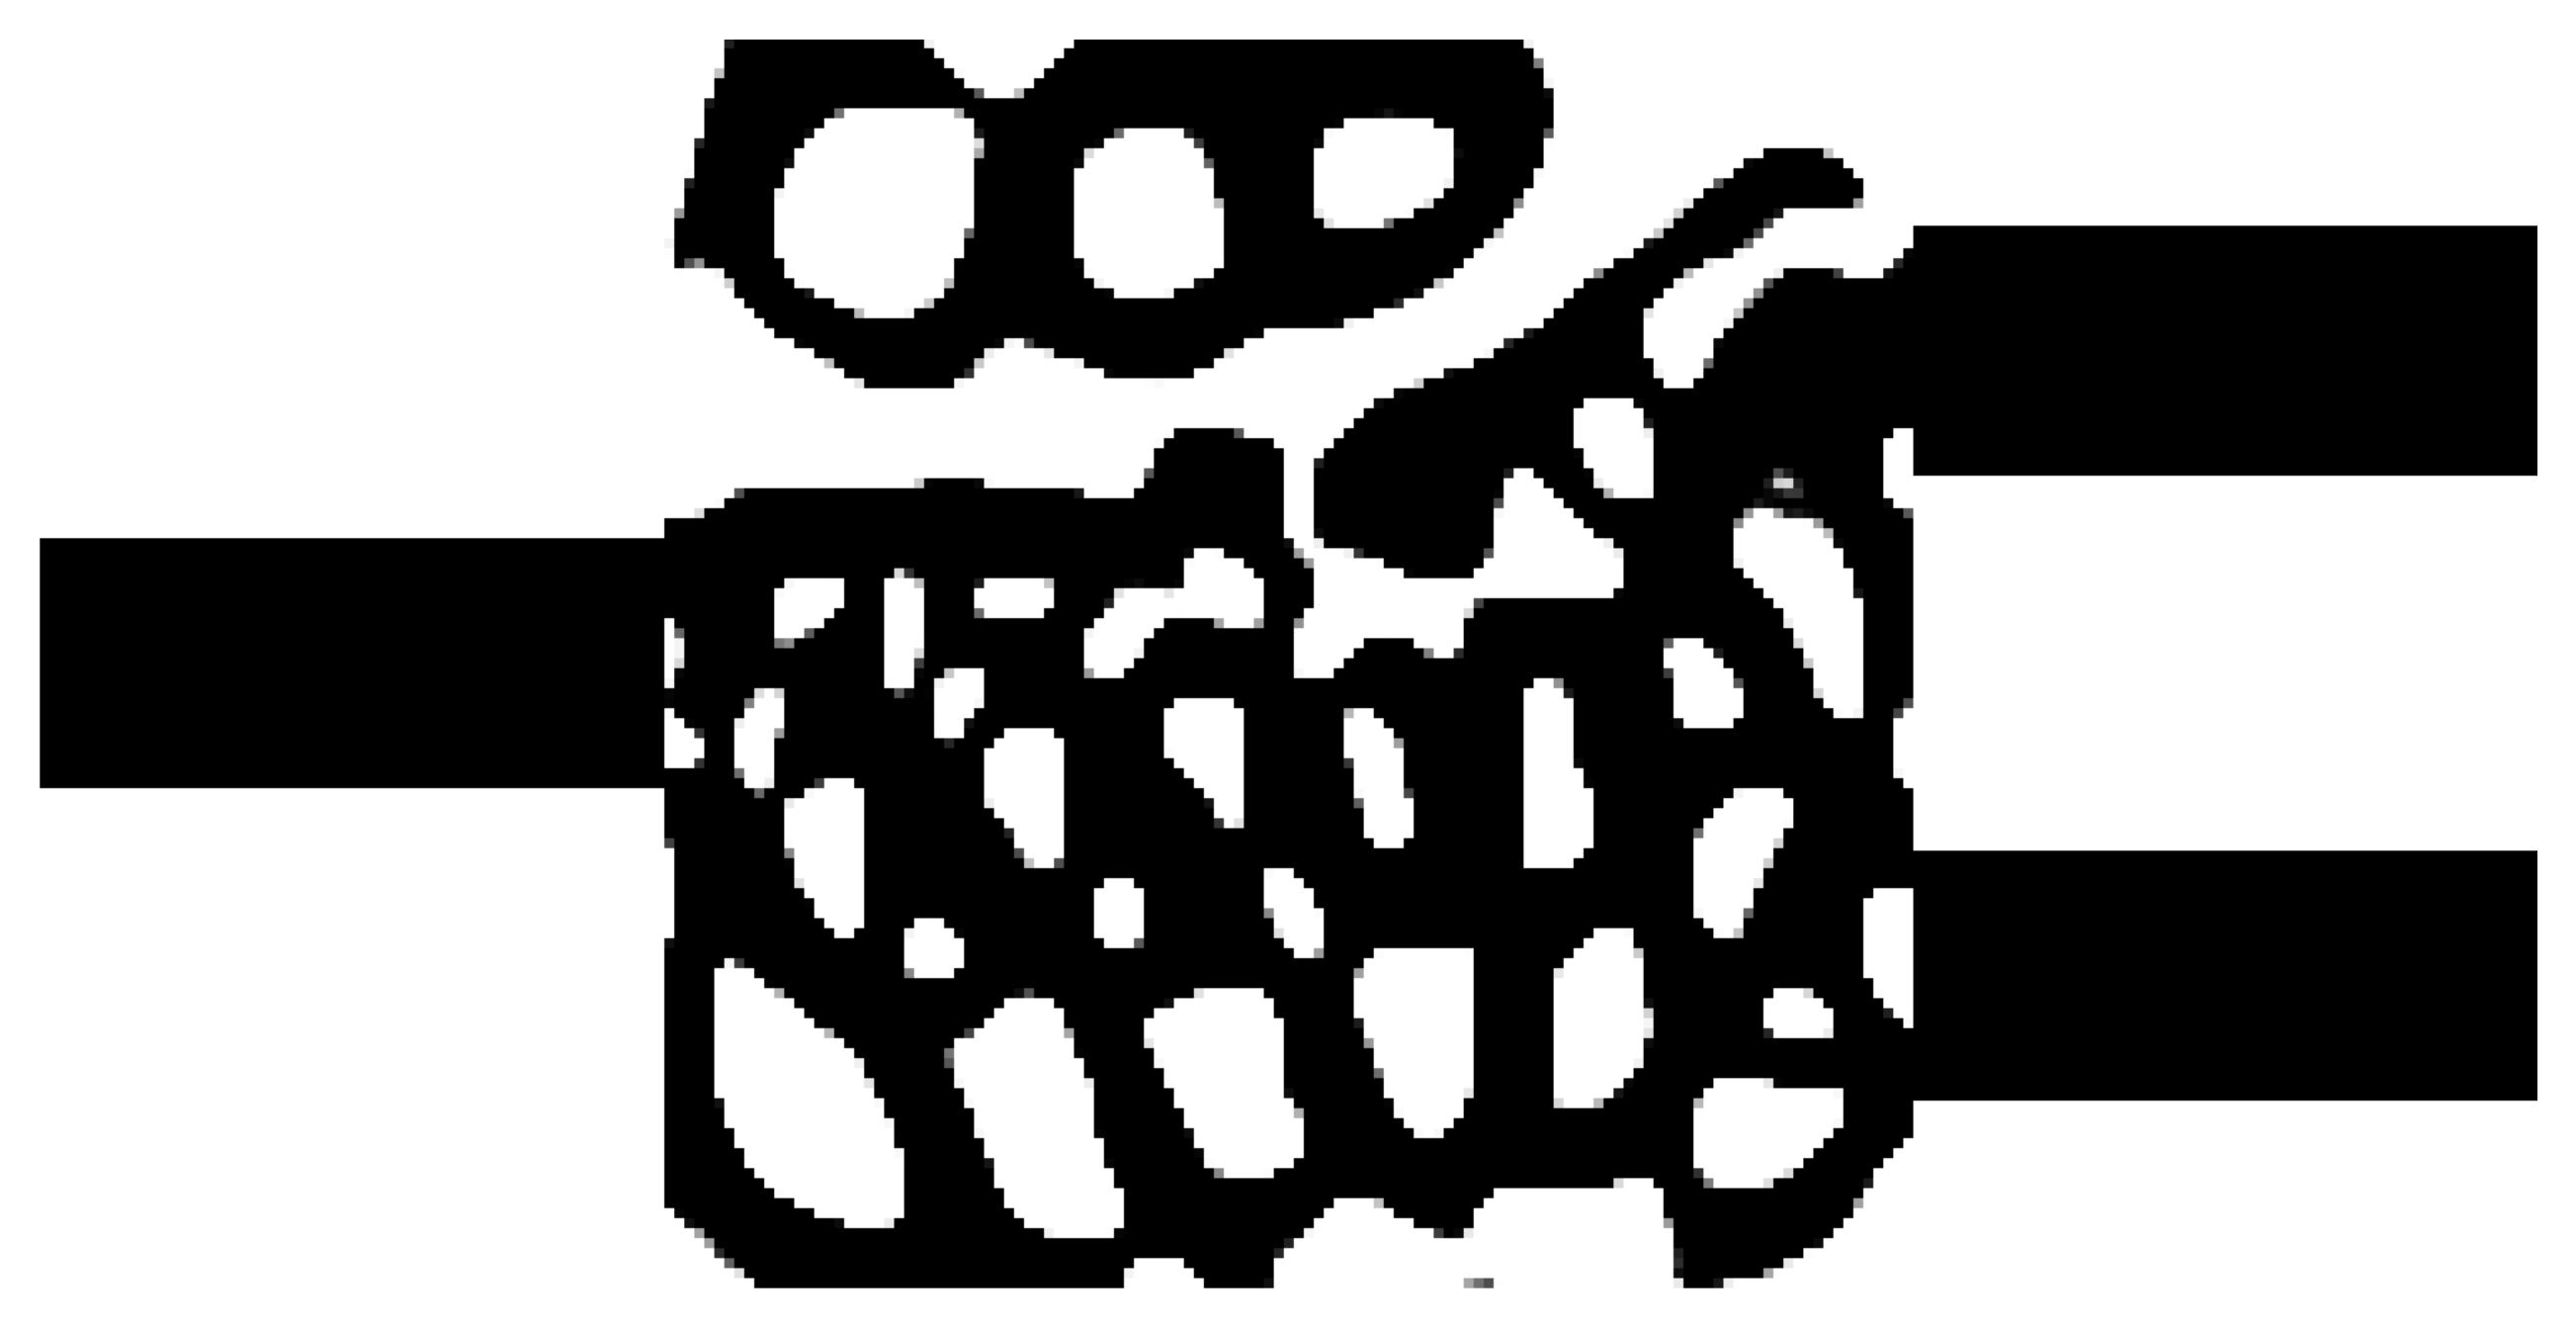
\includegraphics[width=0.35\textwidth]{image/results/wdm/L-BFGS-B/best/eps_eta_i_128.png} &
      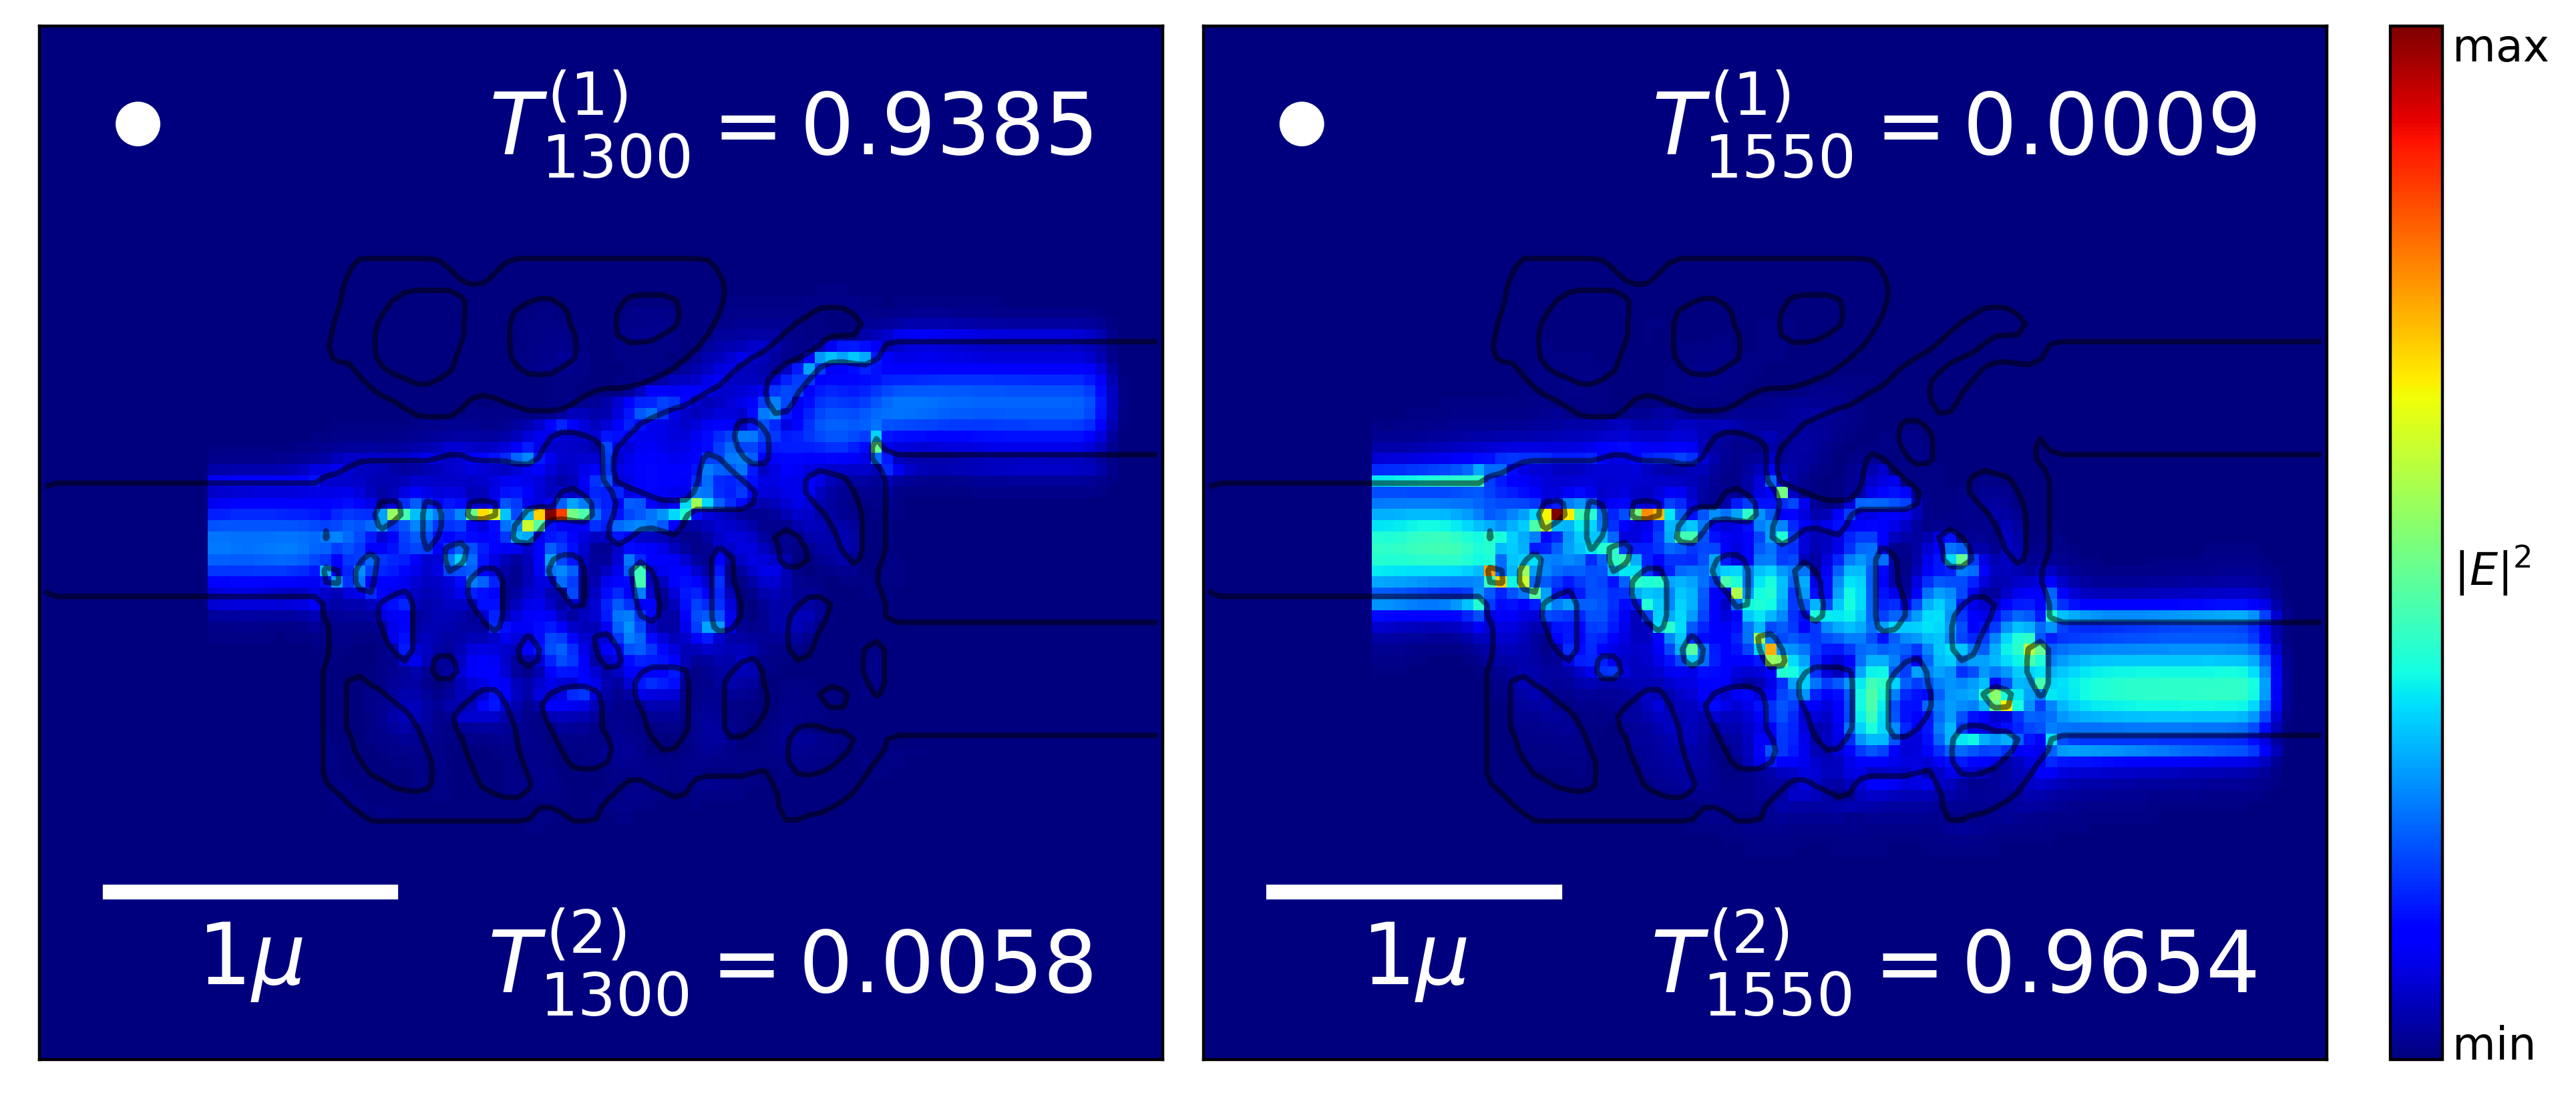
\includegraphics[width=0.60\textwidth]{image/results/wdm/L-BFGS-B/best/field_eta_i_128.png} \\
    \hline
      $\eta_e = 0.55$ &
      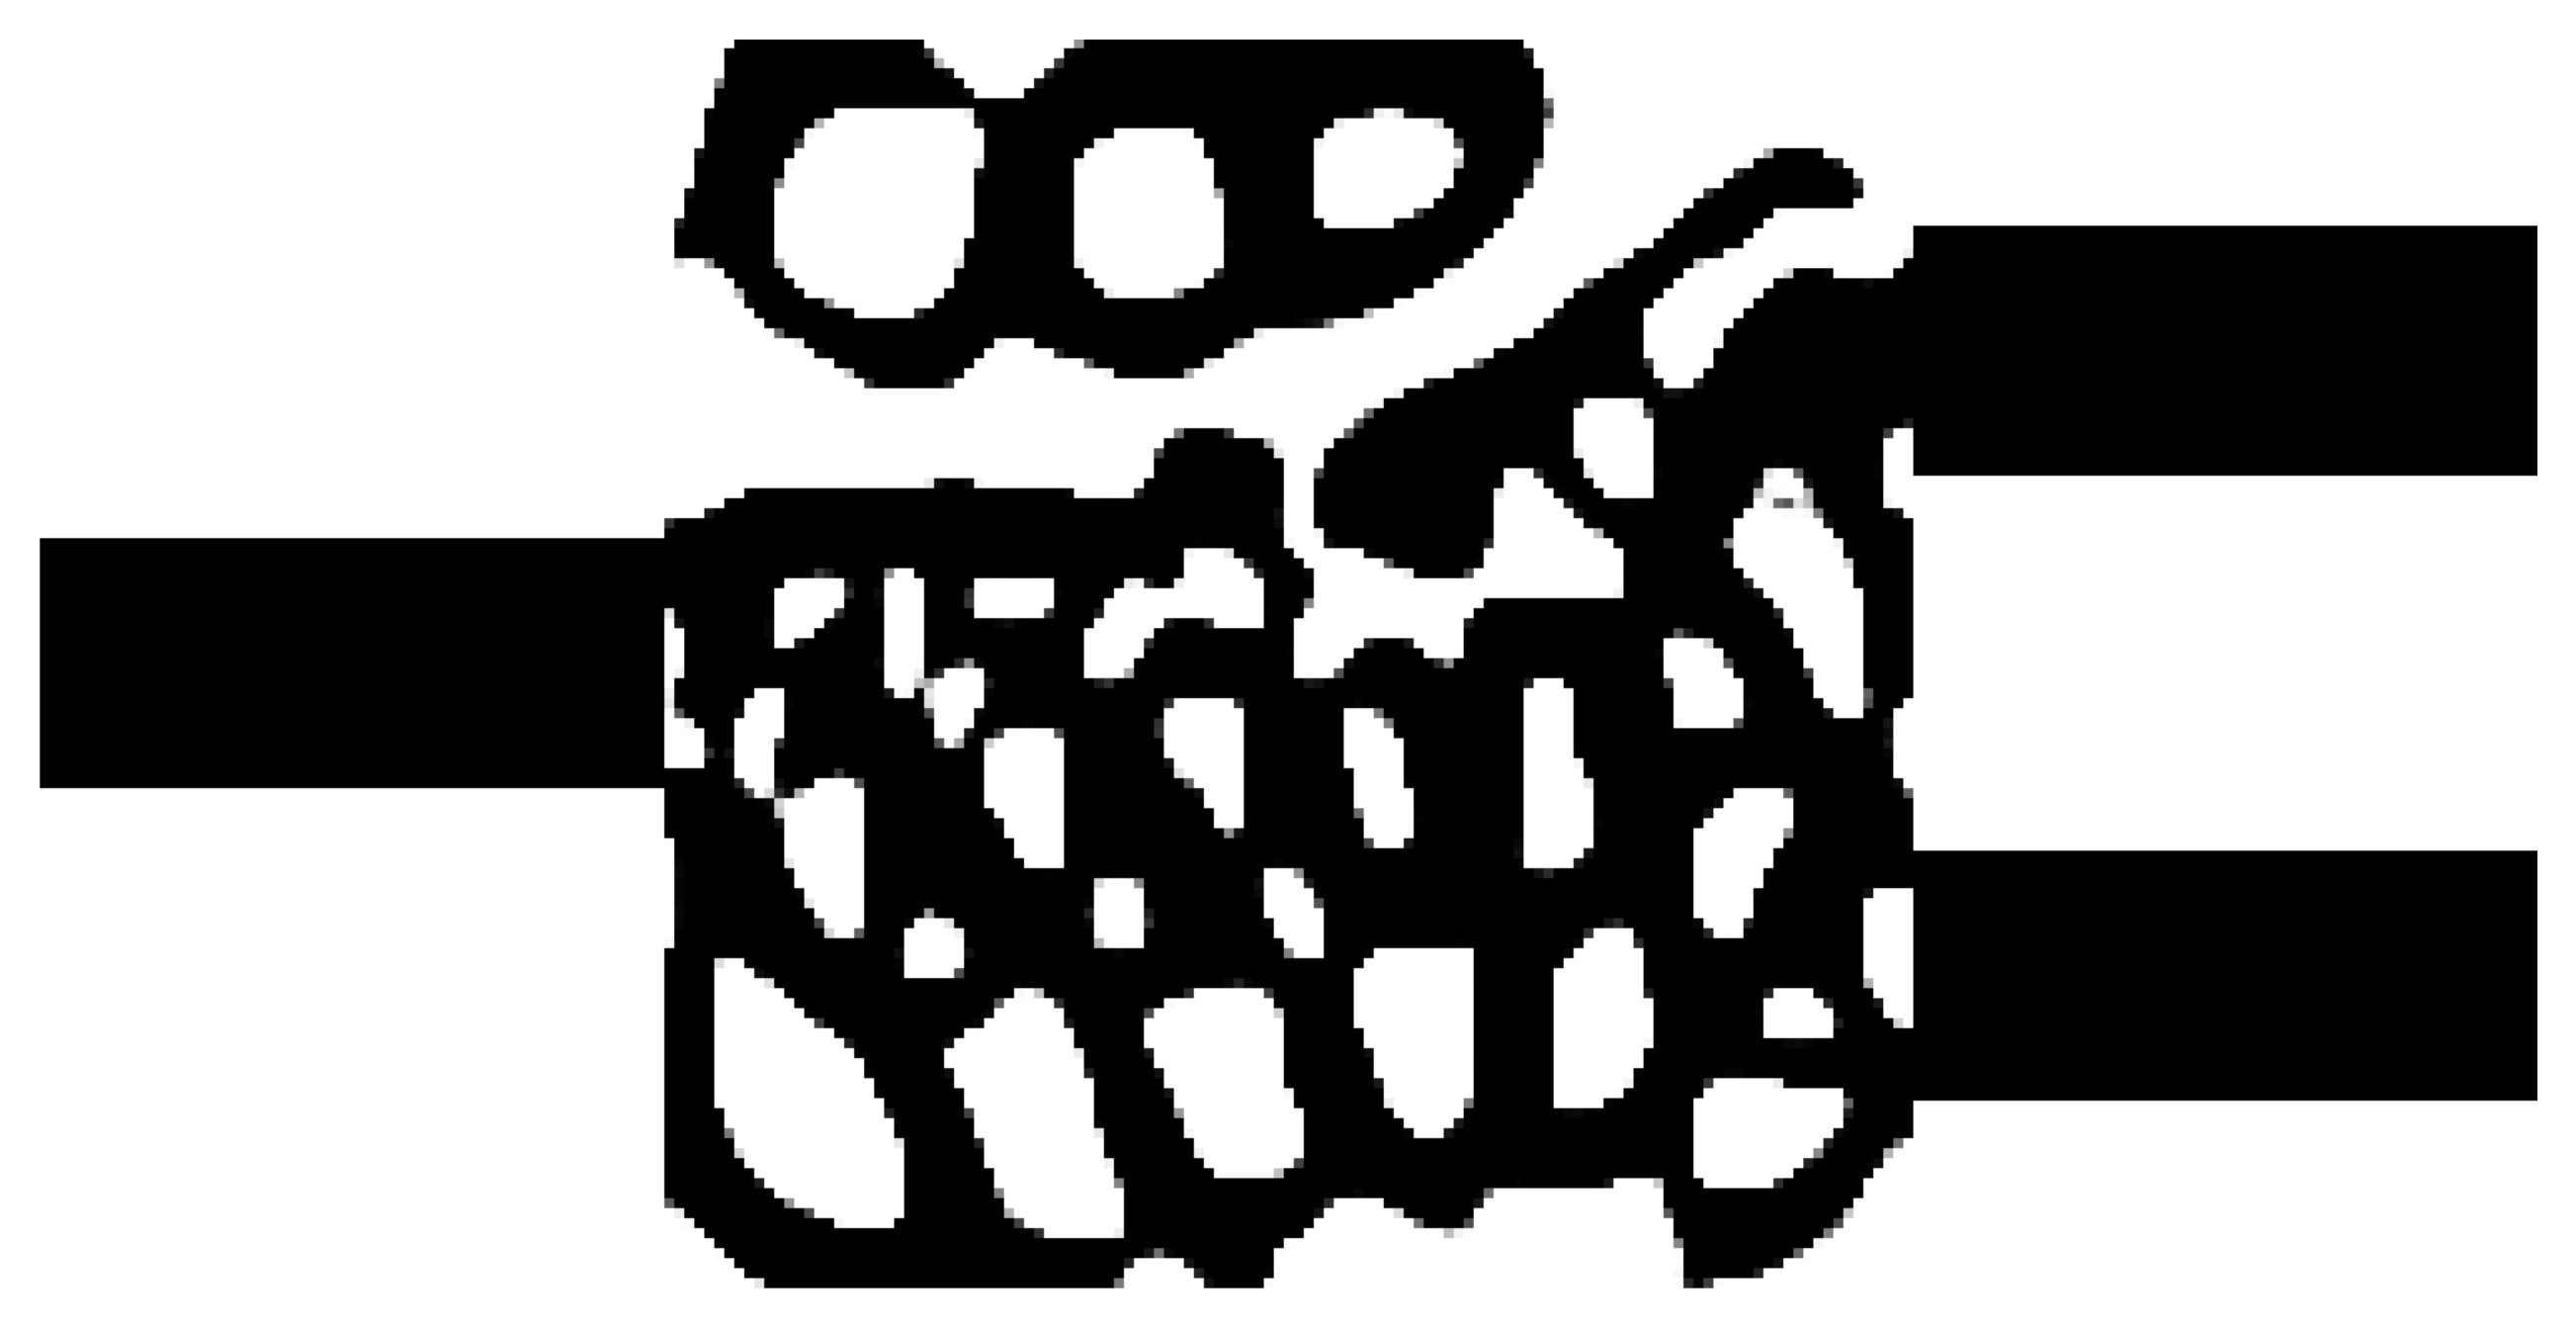
\includegraphics[width=0.35\textwidth]{image/results/wdm/L-BFGS-B/best/eps_eta_e_128.png} &
      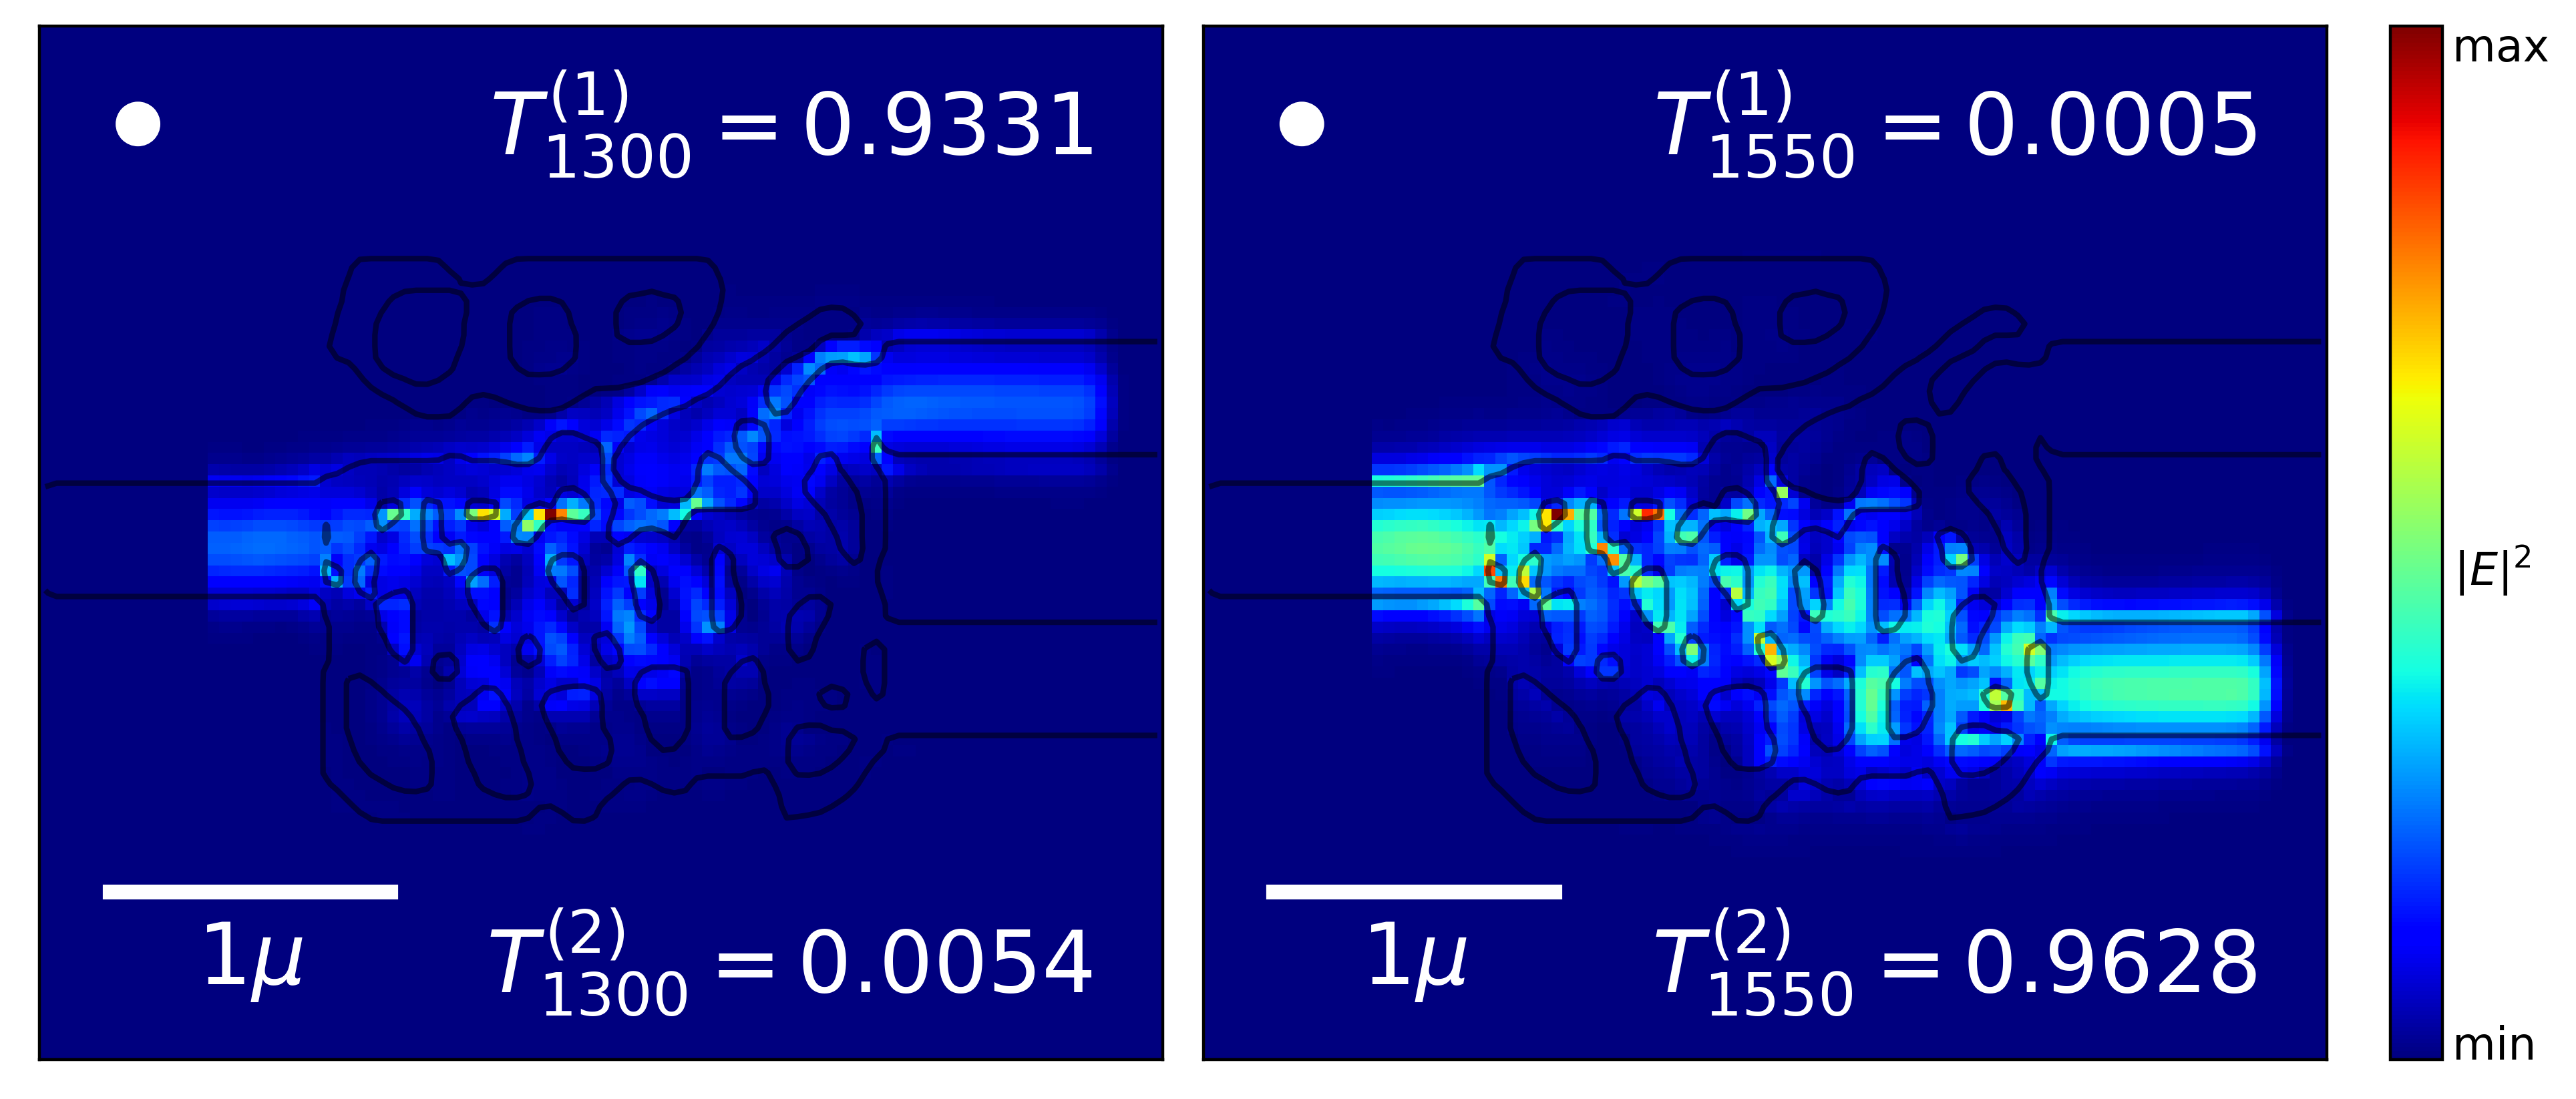
\includegraphics[width=0.60\textwidth]{image/results/wdm/L-BFGS-B/best/field_eta_e_128.png} \\
    \hline
    \end{tabular}
    \hspace*{-3cm}
    \caption{Mejores diseños del WDM usando L-BFGS-B ($seed = 128$). 
    Las imágenes de la primera fila corresponden al diseño dilatado ($\eta_d$), 
    las de la segunda fila al diseño nominal ($\eta_i$) y la tercera fila al diseño erosionado ($\eta_e$).}
    \label{tab:best-bend-L-BFGS-B}
\end{table}

